%%%%%%%%%%%% Selective edge pruning %%%%%%%%%%%%
\chapter{Selective edge pruning} \label{s:ap:sel_prun}

% Leiden vs SBM
\section{Leiden vs SBM} \label{s:ap:leiden_sbm}

% Comunity sizes
\begin{figure}[!h]
    \centering
    \begin{subfigure}[!t]{1.0\textwidth}
        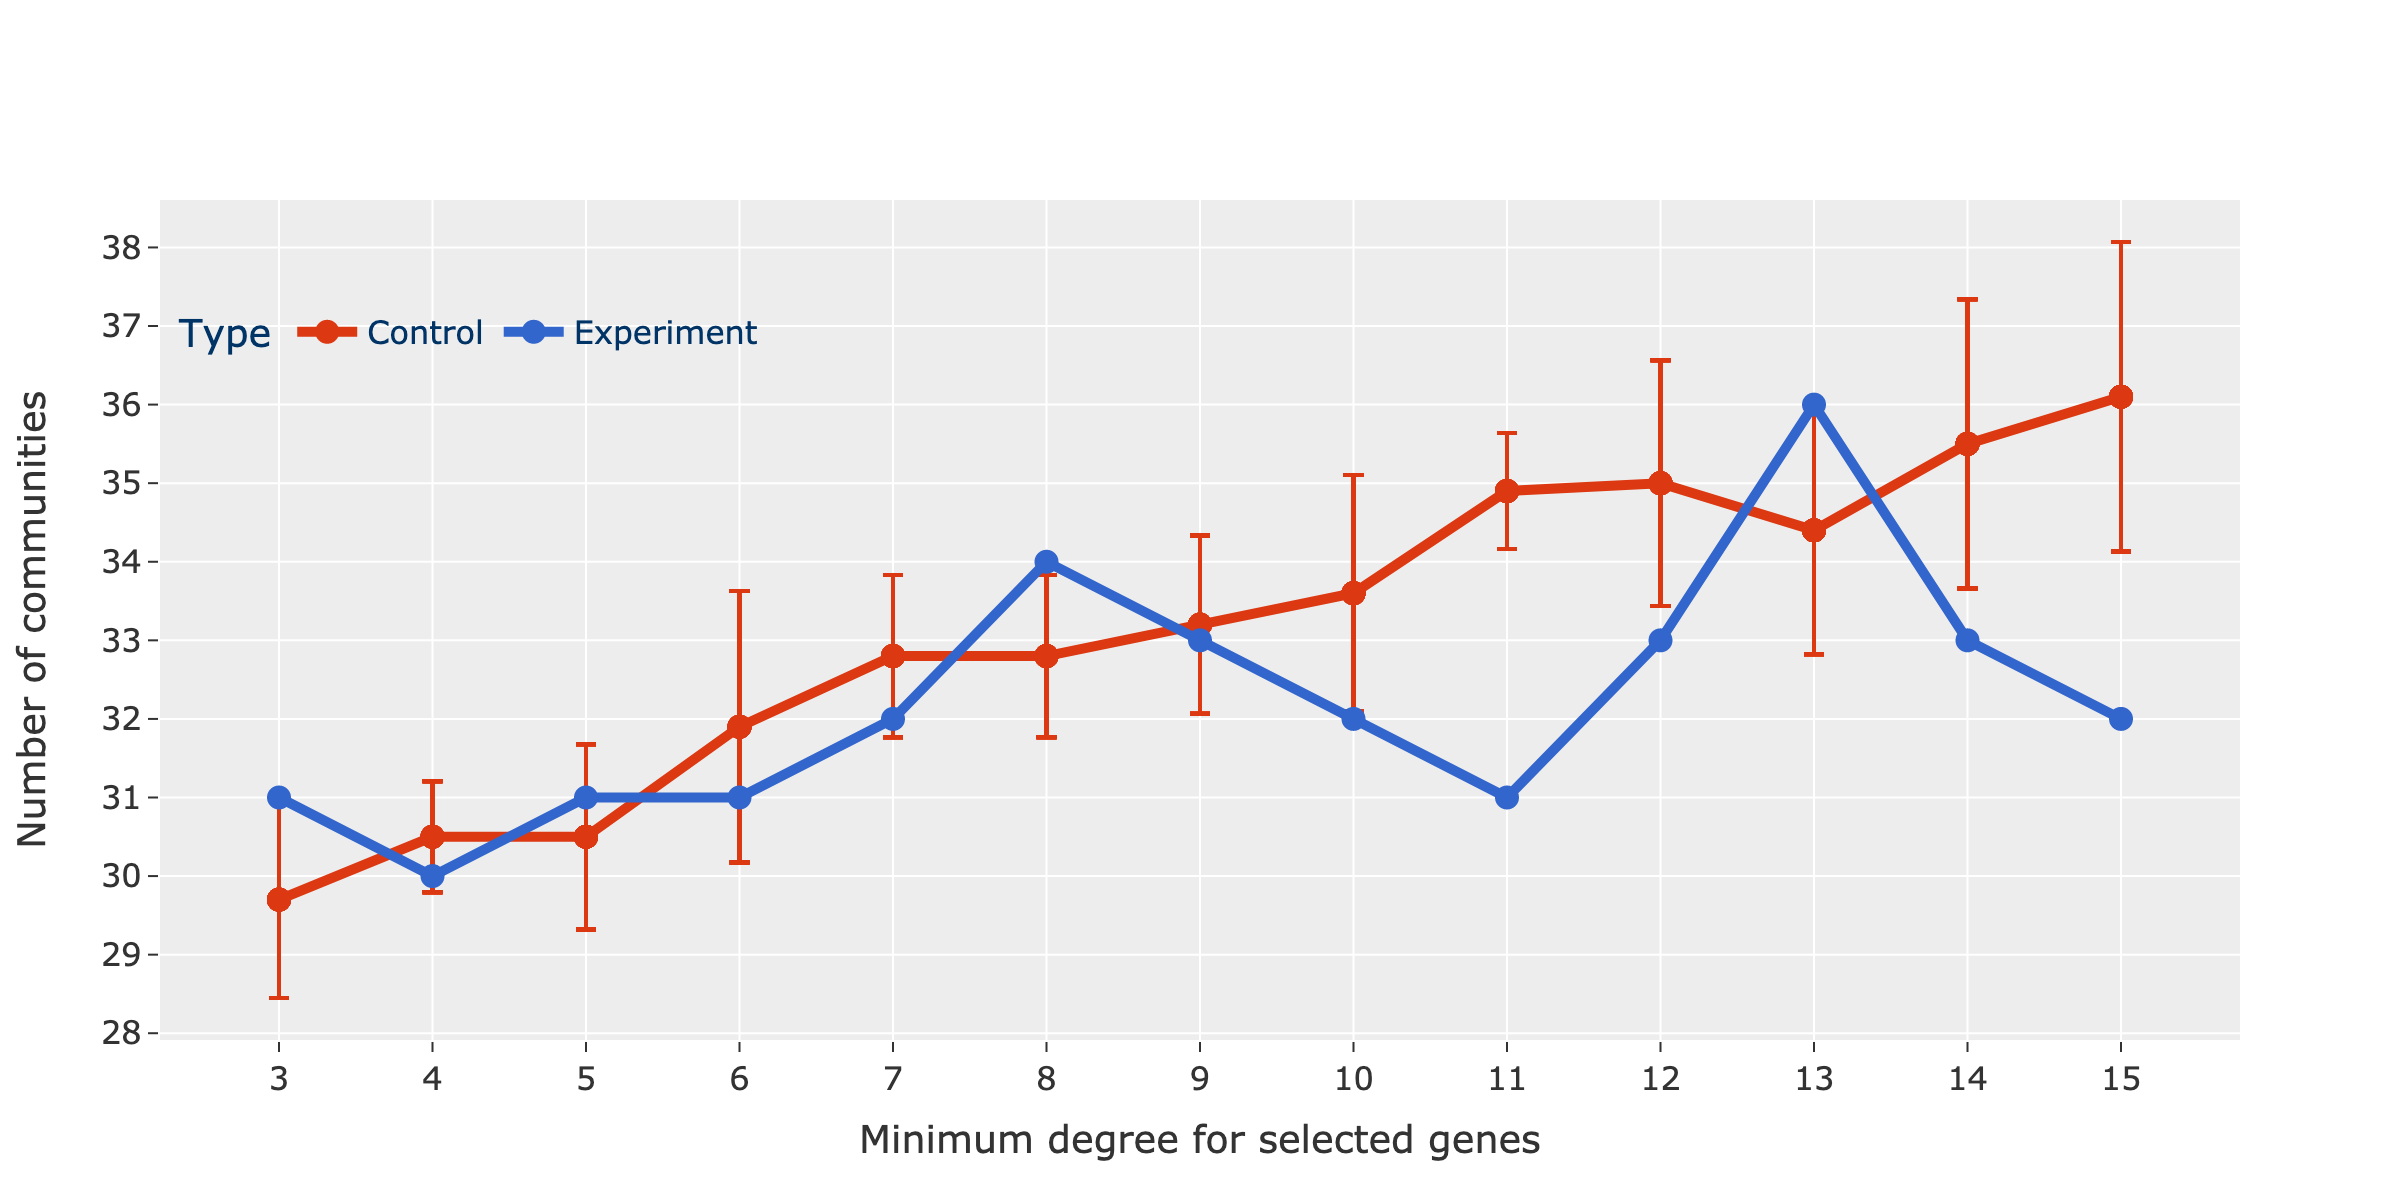
\includegraphics[width=\textwidth]{Sections/Network_I/Resources/selective_pruning/com_comp/sbm_comNum_sel_prun.png}
        \caption{SBM}
        \label{fig:ap:sbm_com_size}
    \end{subfigure} 
    \begin{subfigure}[!t]{1.0\textwidth}
        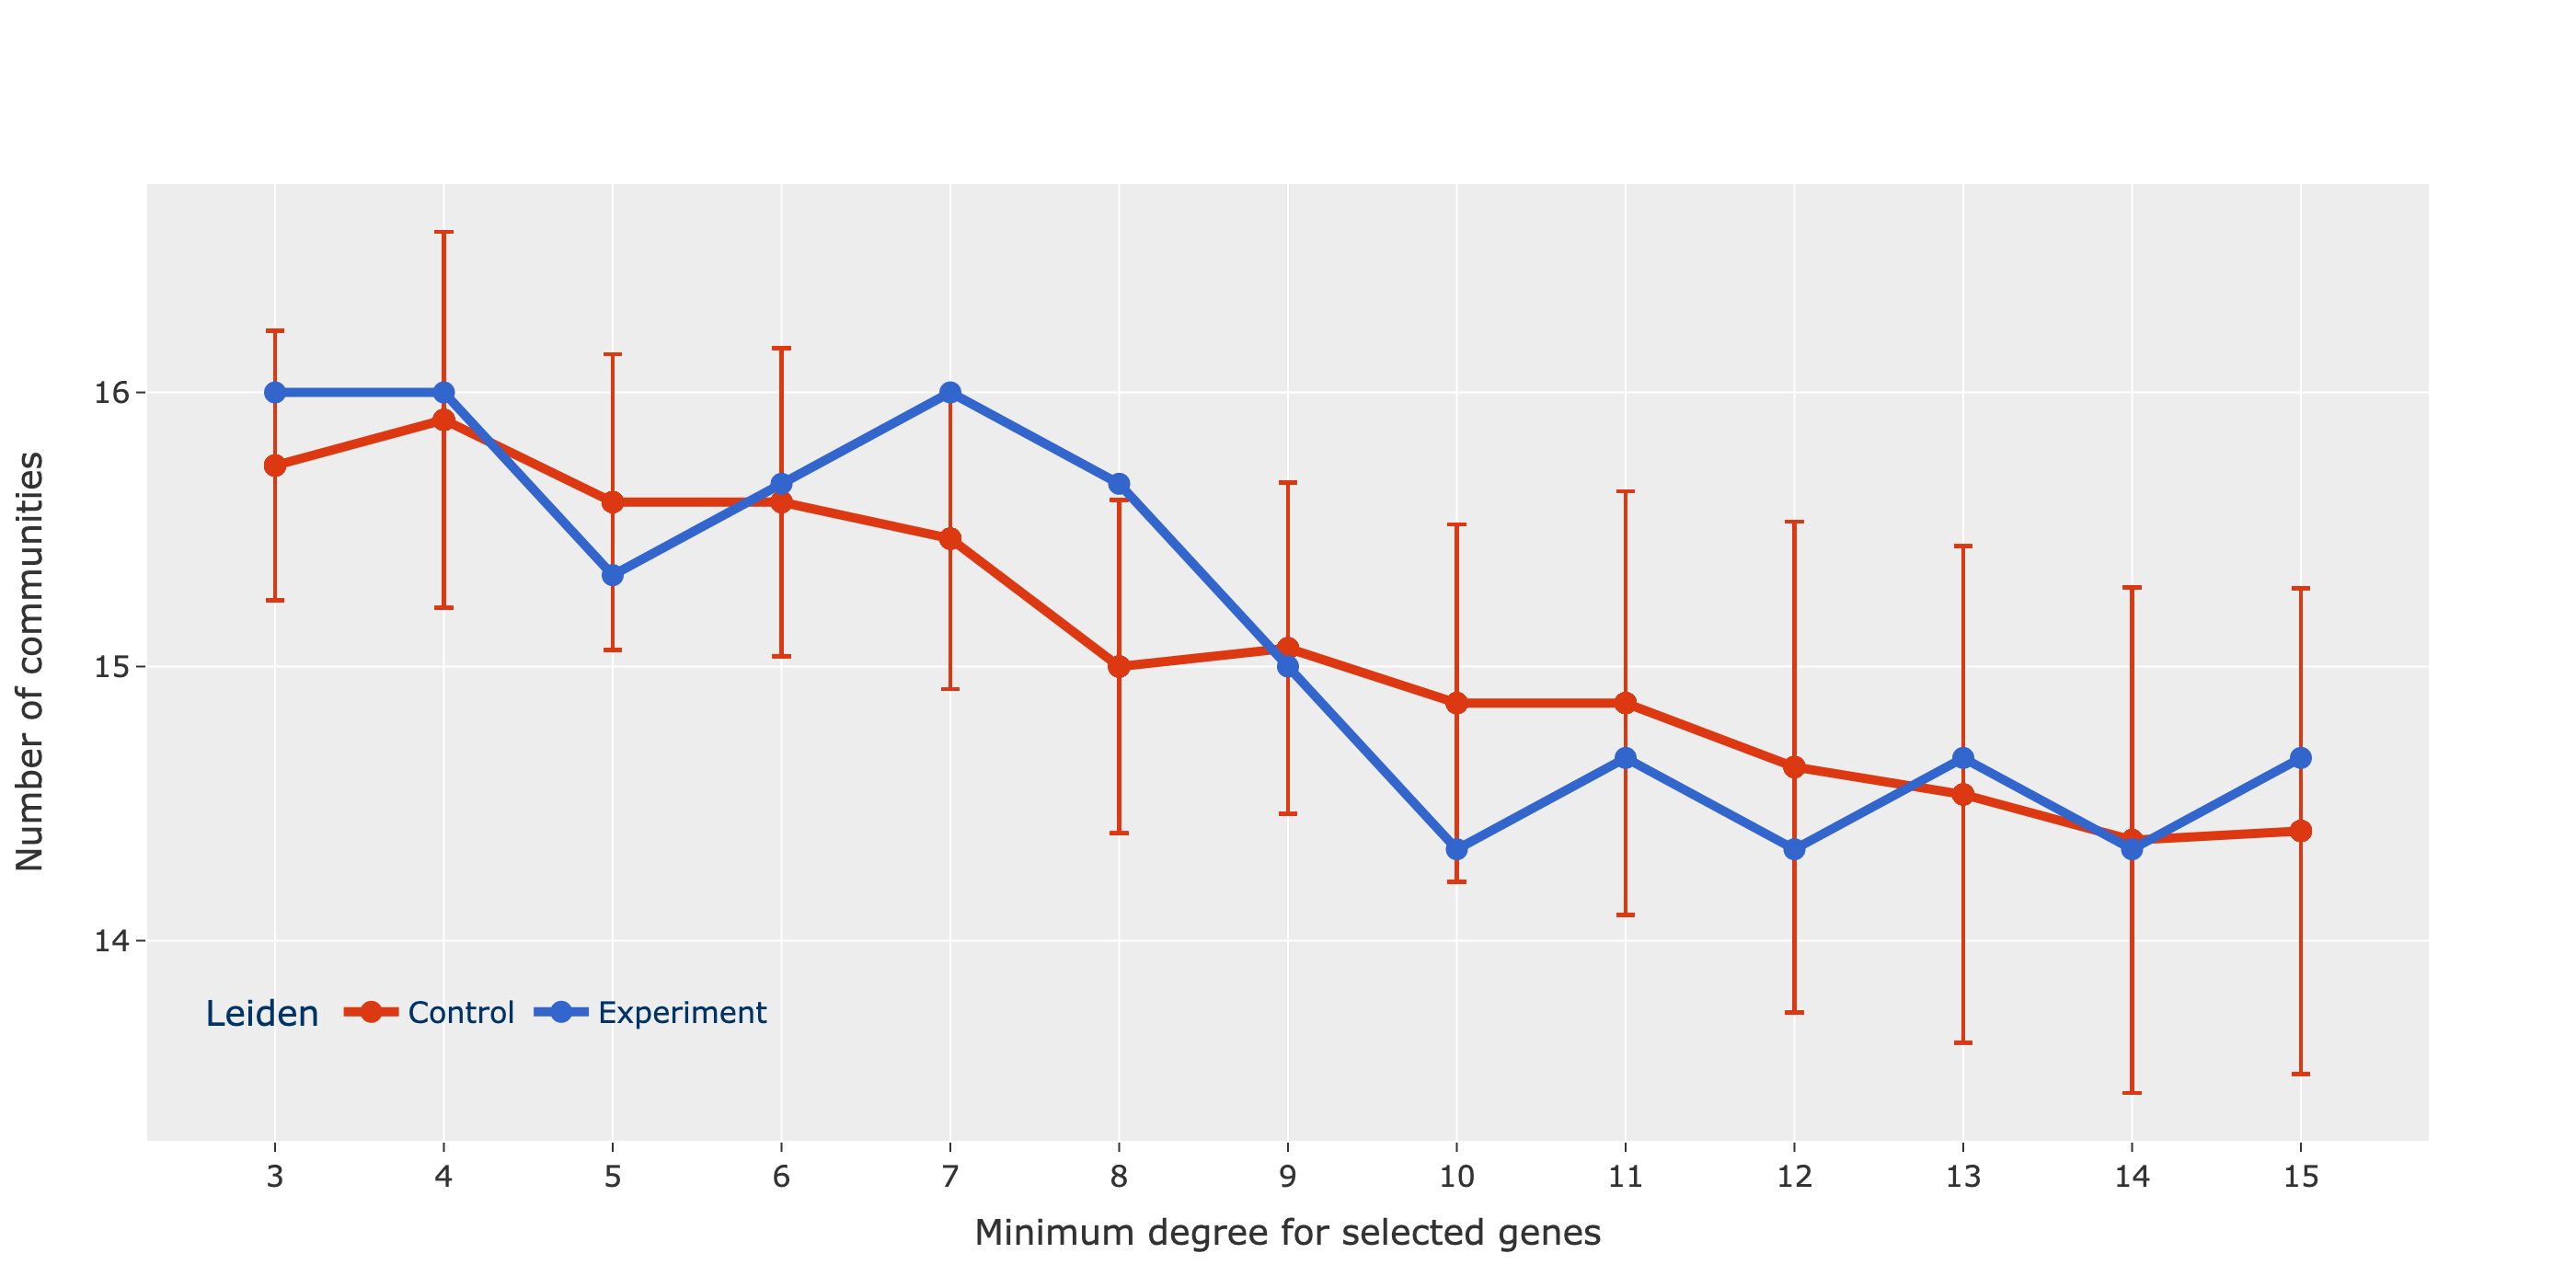
\includegraphics[width=\linewidth]{Sections/Network_I/Resources/selective_pruning/leid_comNum_sel_prun.png}
        \caption{Leiden}
        \label{fig:ap:leid_com_size}
    \end{subfigure}\hspace{\fill}  
    \caption{Community size comparison between Leiden and SBM. This serves as a supporting material to the work done in \cref{s:N_I:sel_pruning}}
    \label{fig:ap:com_size_comp}
\end{figure}


\section{Clustering dendrogram} \label{s:ap:leiden_sbm}

%  Morpheus hierarchical clustering
\begin{figure}[!htb]   
\centering
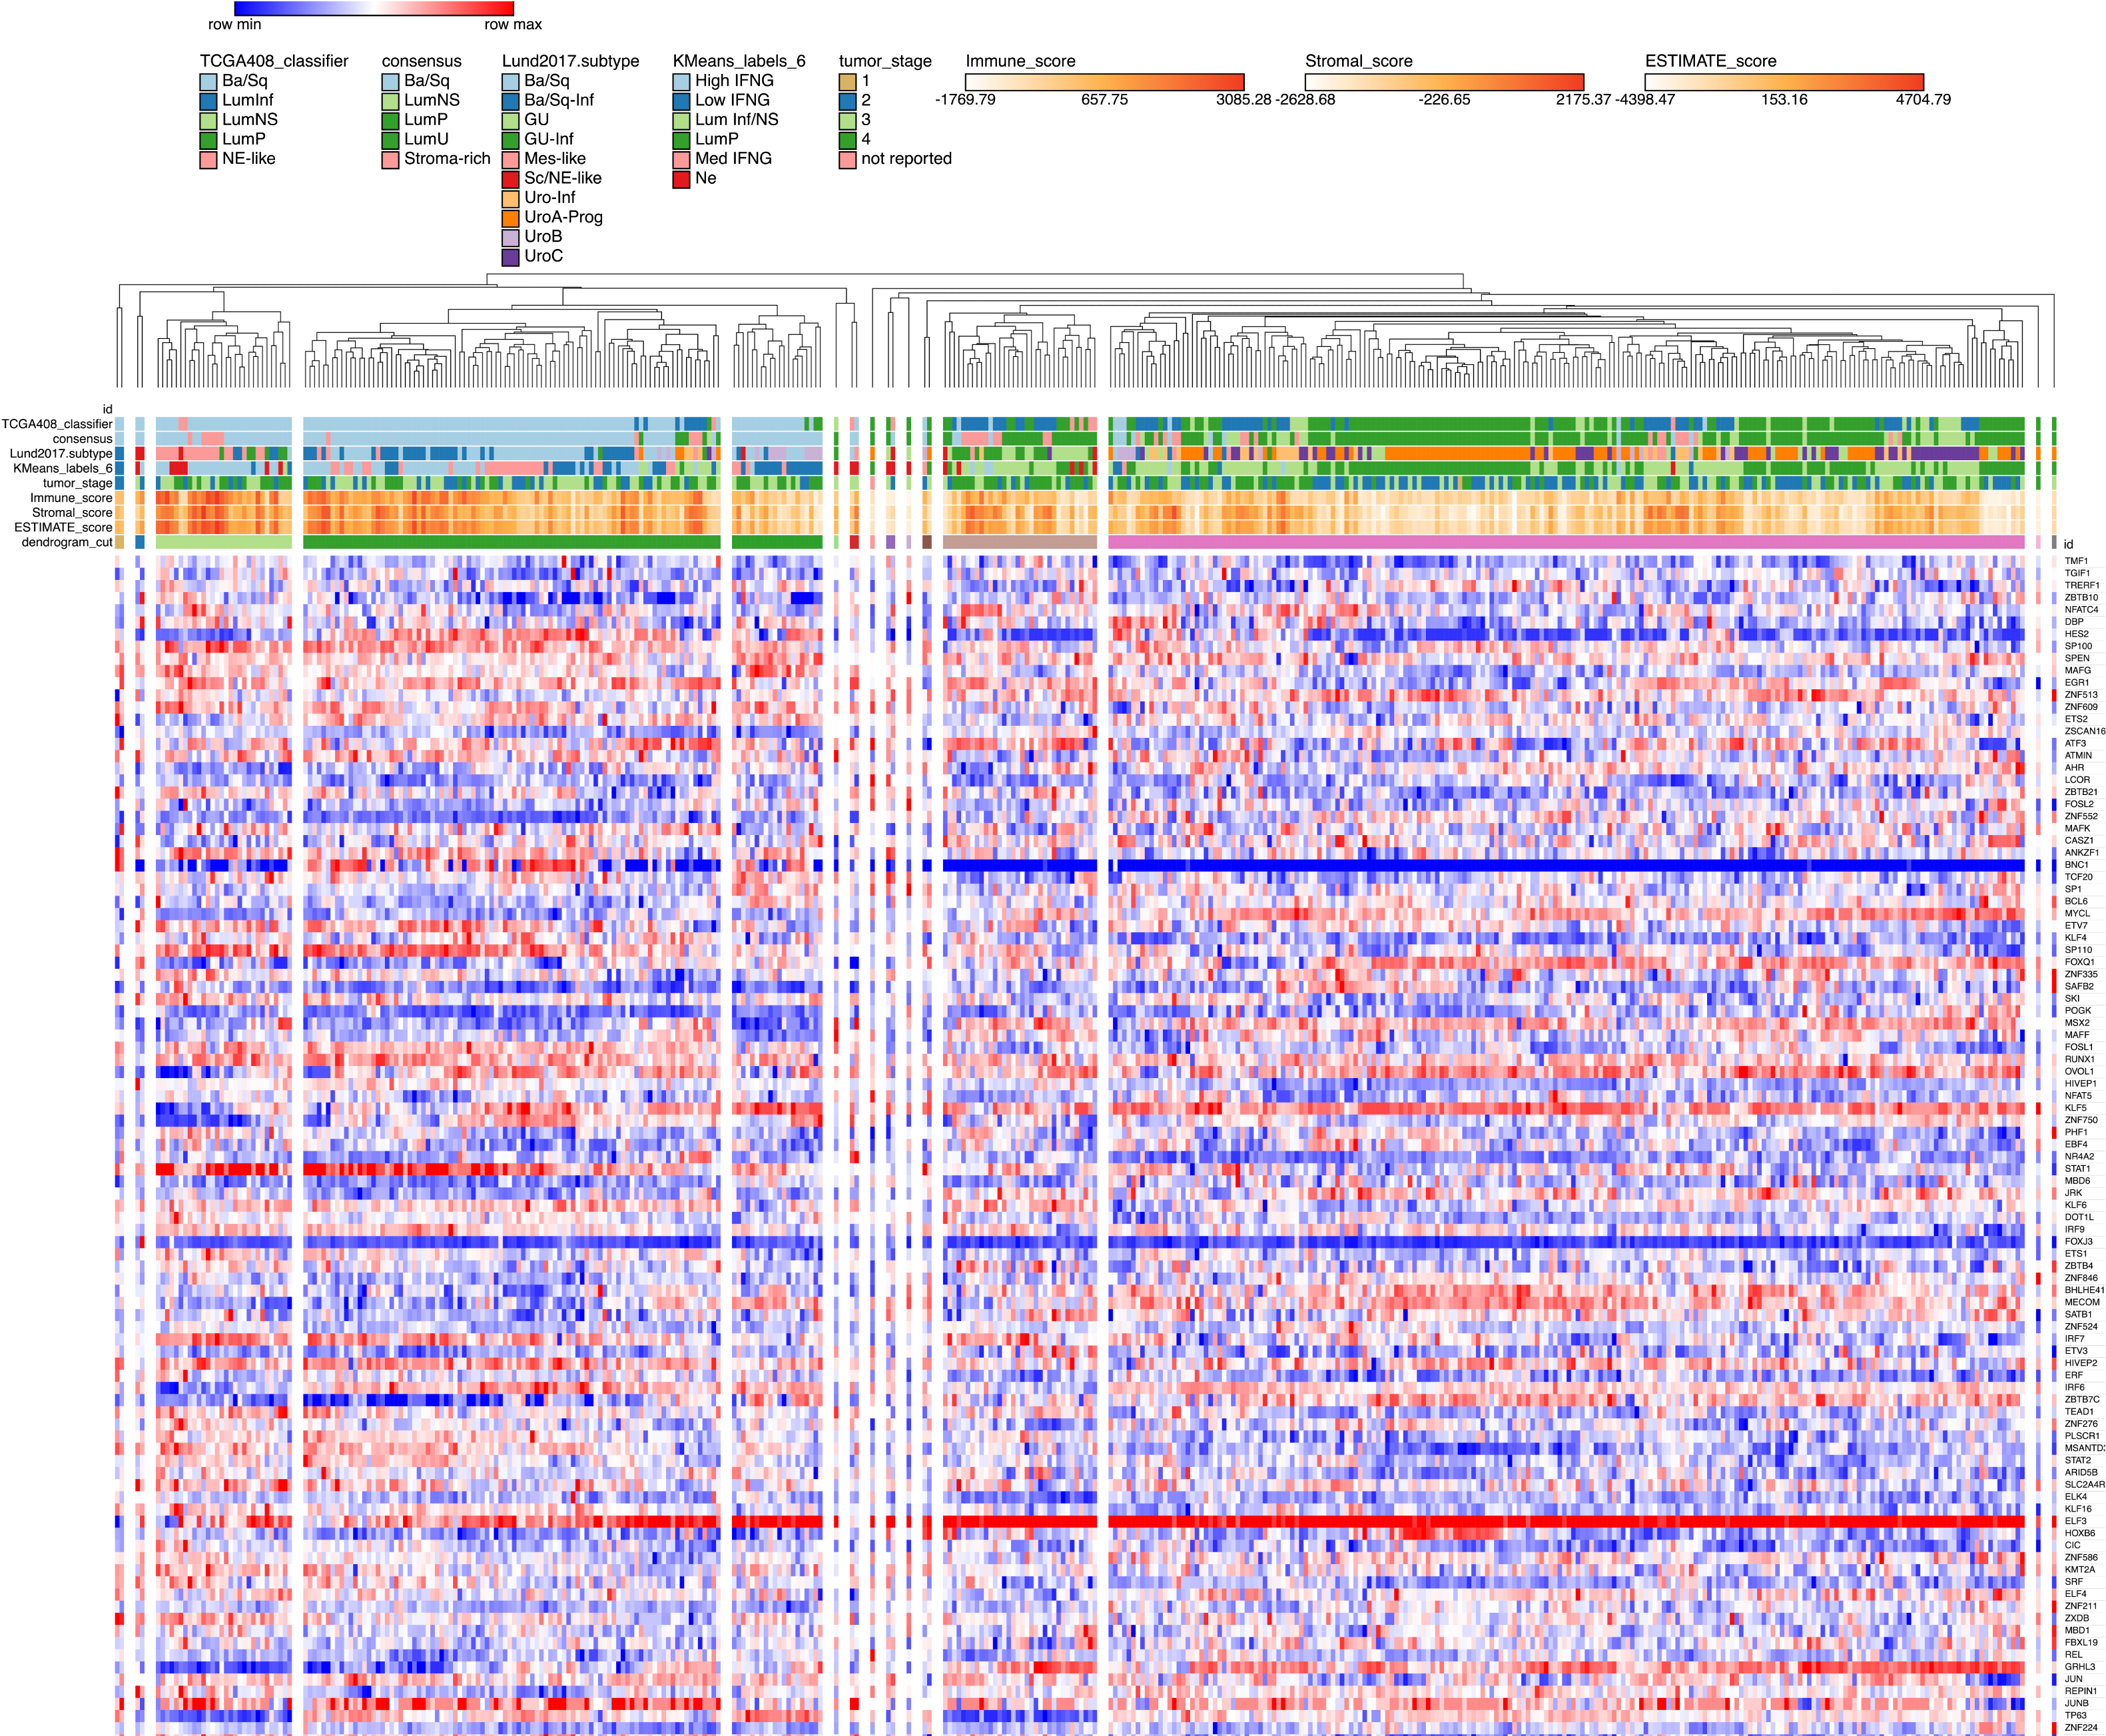
\includegraphics[width=1.0\textwidth,keepaspectratio]{Sections/Network_I/Resources/selective_pruning/15_CS_norm_sel_tfs.png}
  \caption{Hierarchical clustering of the 98 TFs found in \cref{s:N_I:sel_tfs}. The columns at the top of the heatmap represents the previous classification (TCGA \cite{Robertson2017-mg}, Consensus \cite{Kamoun2020-tj}, Lund \cite{Marzouka2018-ge} and the stratification from \cref{s:clustering_analysis}) as well as the Immune, Stromal and ESTIMATE scores available with the TCGA cohort.}
\label{fig:ap:morph_sel_tfs}
\end{figure}

\section{Tumour vs Non-tumour gene expression} \label{s:ap:tum_vs_non-tumour}


\Cref{fig:ap:sel_tfs_mean} depicts the mean expression of the 98 TFs genes found in the previous subsection. The log plot shows the non-cancerous mean on the y-axis and the tumour mean expression on the x-axis, the size and colour of the points is proportional to the mutation burden across the MIBC cohort from TCGA. The genes higher on the y-axis have a higher expression in the non-cancerous, similarly for x-axis, further on the right hand side, higher average value in the tumour cohort. \textit{ELF3} it is on the top right corner meaning that it is expressed both in the tumour and non-cancerous datasets, and it is also highly mutated in MIBC. \textit{BNC1} is on he left corner, having lower expression across the samples.

% Tum vs non-cancerous dataset.
\begin{figure}[!htb]   
\centering
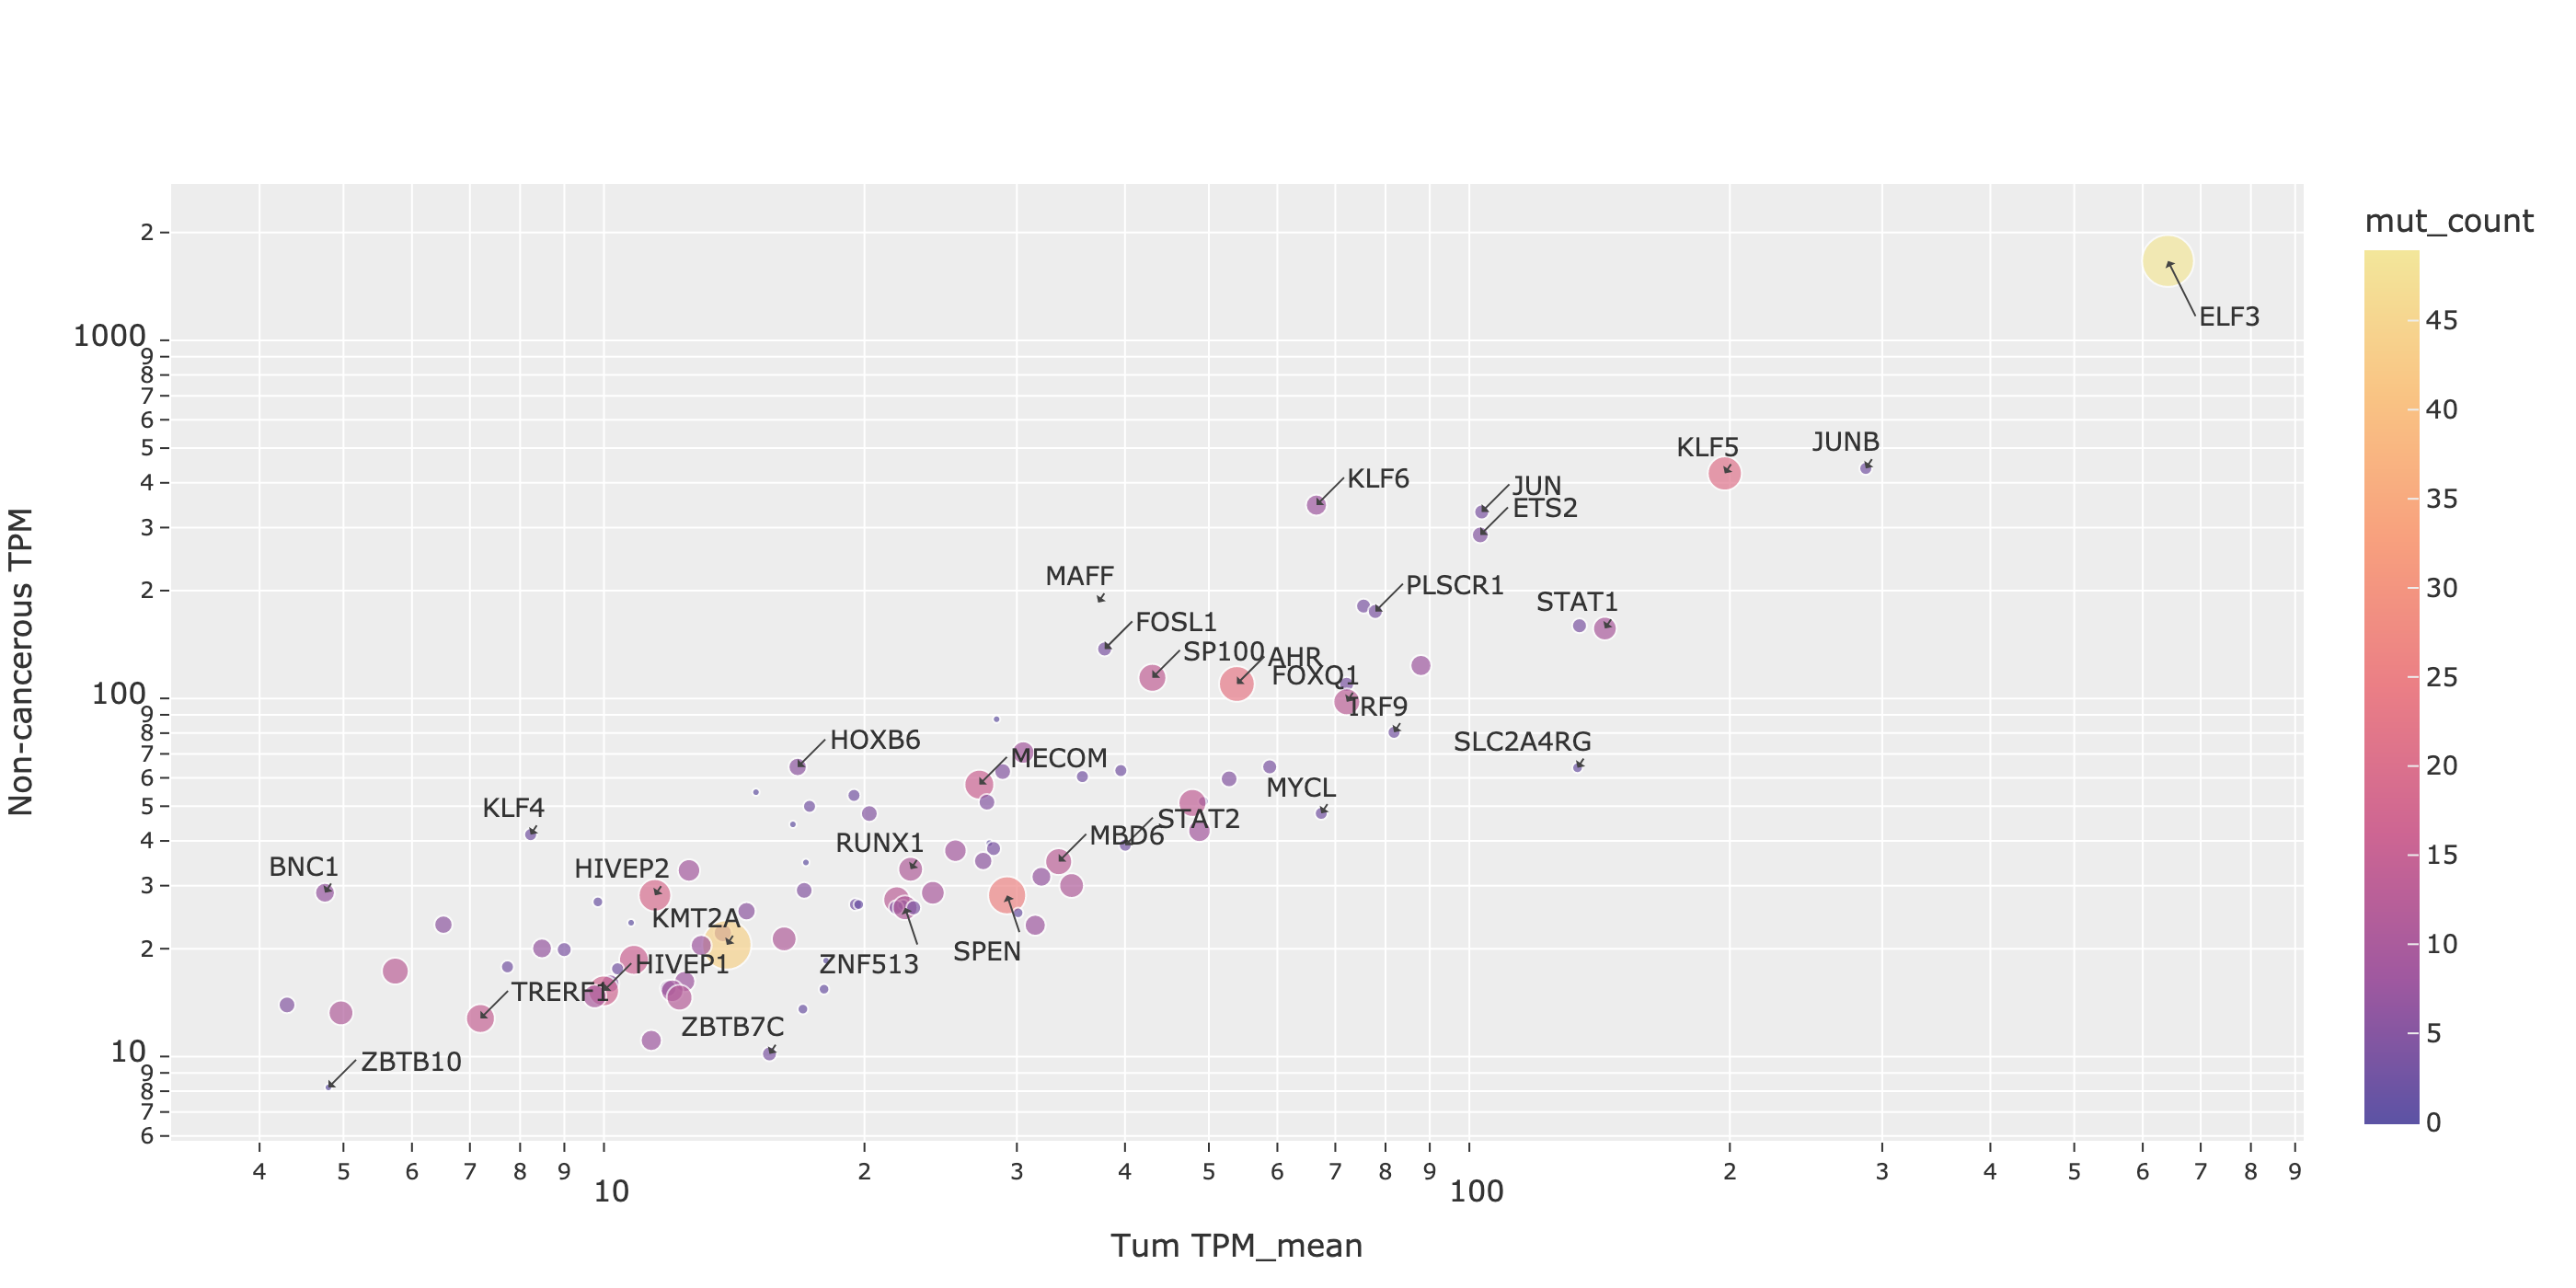
\includegraphics[width=1.0\textwidth,height=1.0\textheight,keepaspectratio]{Sections/Network_I/Resources/selective_pruning/sel_tfs/sel_tfs_mean_tum_healthy.png}
  \caption{Selected TFs expression in the MIBC TCGA cohort and in the non-cancerous. Both the colour and size of the points are proportional to the mutation burden in the TCGA cohort.}
\label{fig:ap:sel_tfs_mean}
\end{figure}


% Metadata of the hierarchical clustering
\section{TCGA metadata and the clusters based on the 98 TFs} \label{s:ap:sel_prun_tcga_meta}


\begin{figure}[!htb]   
    \centering
    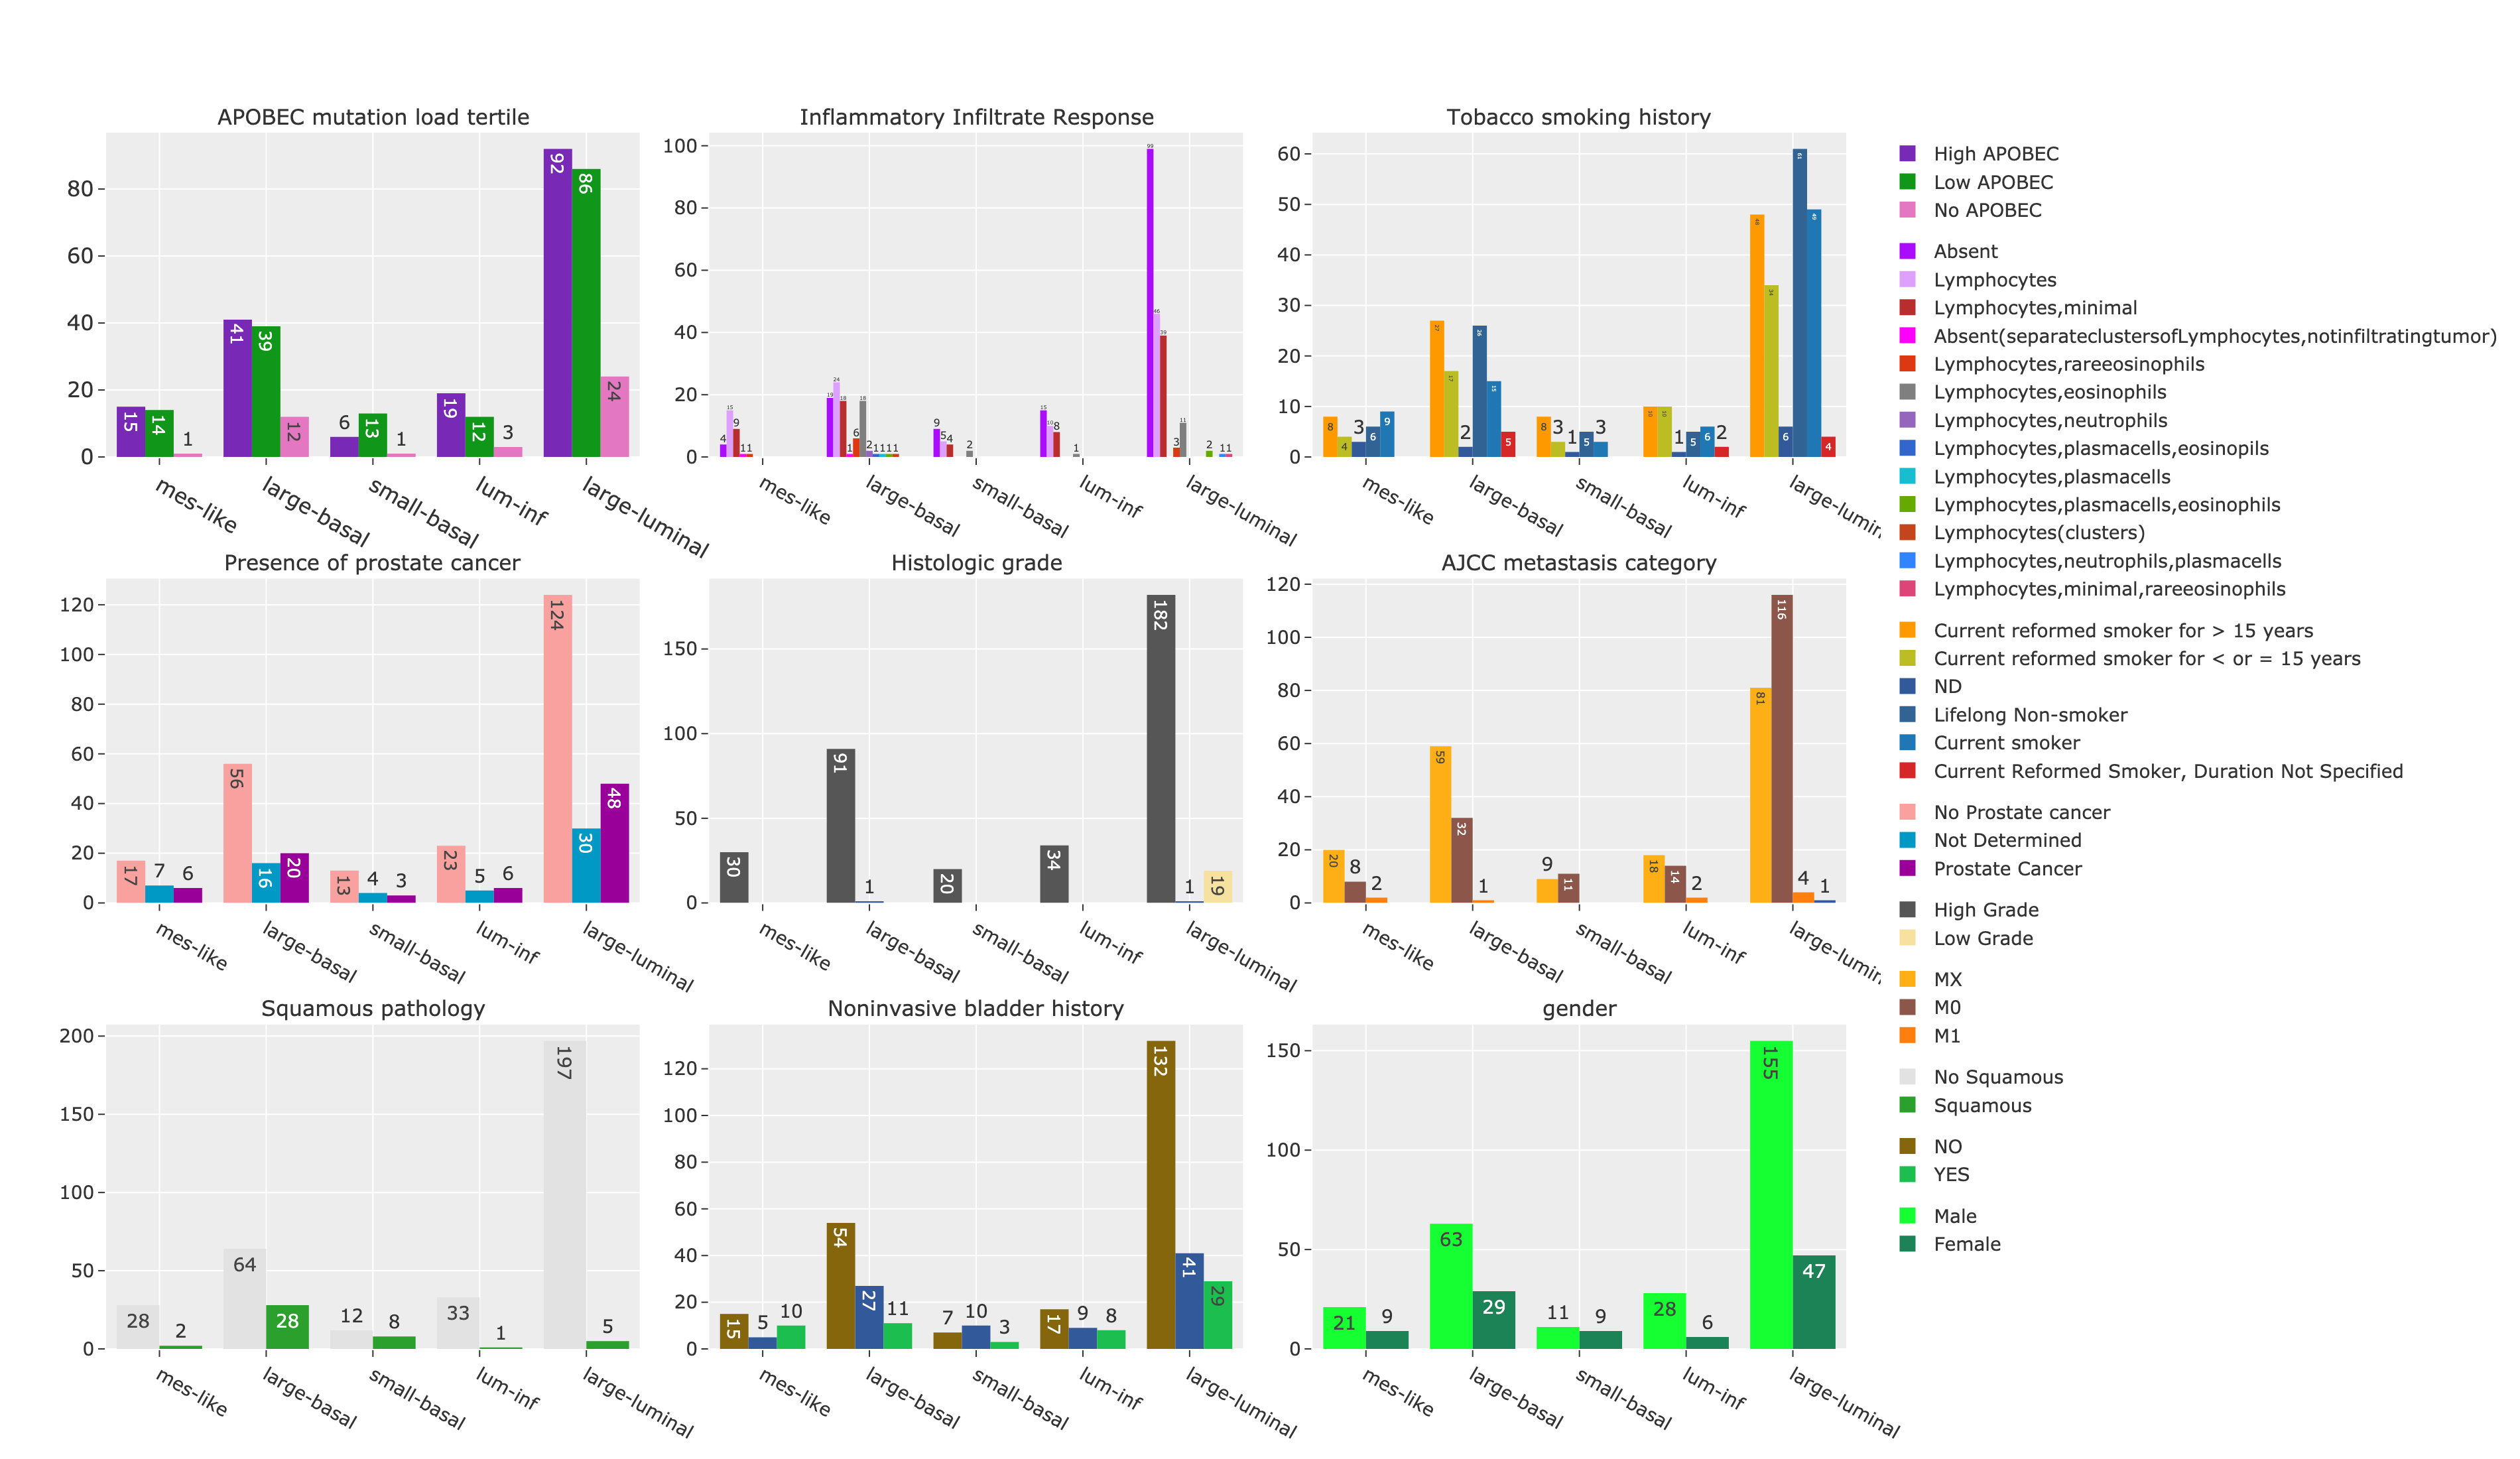
\includegraphics[width=1.0\textwidth,keepaspectratio]{Sections/Network_I/Resources/selective_pruning/sel_tfs/sel_tfs_tcga_meta.png}
      \caption{The metadata from TCGA \cite{Robertson2017-mg} across the subtypes derived from applying hierarchical clustering on the expression of the 98 TFs from \cref{fig:N_I:sel_tfs}. }
    \label{fig:ap:sel_tfs_tcga_metadata}
\end{figure}

\begin{figure}[!htb]   
    \centering
    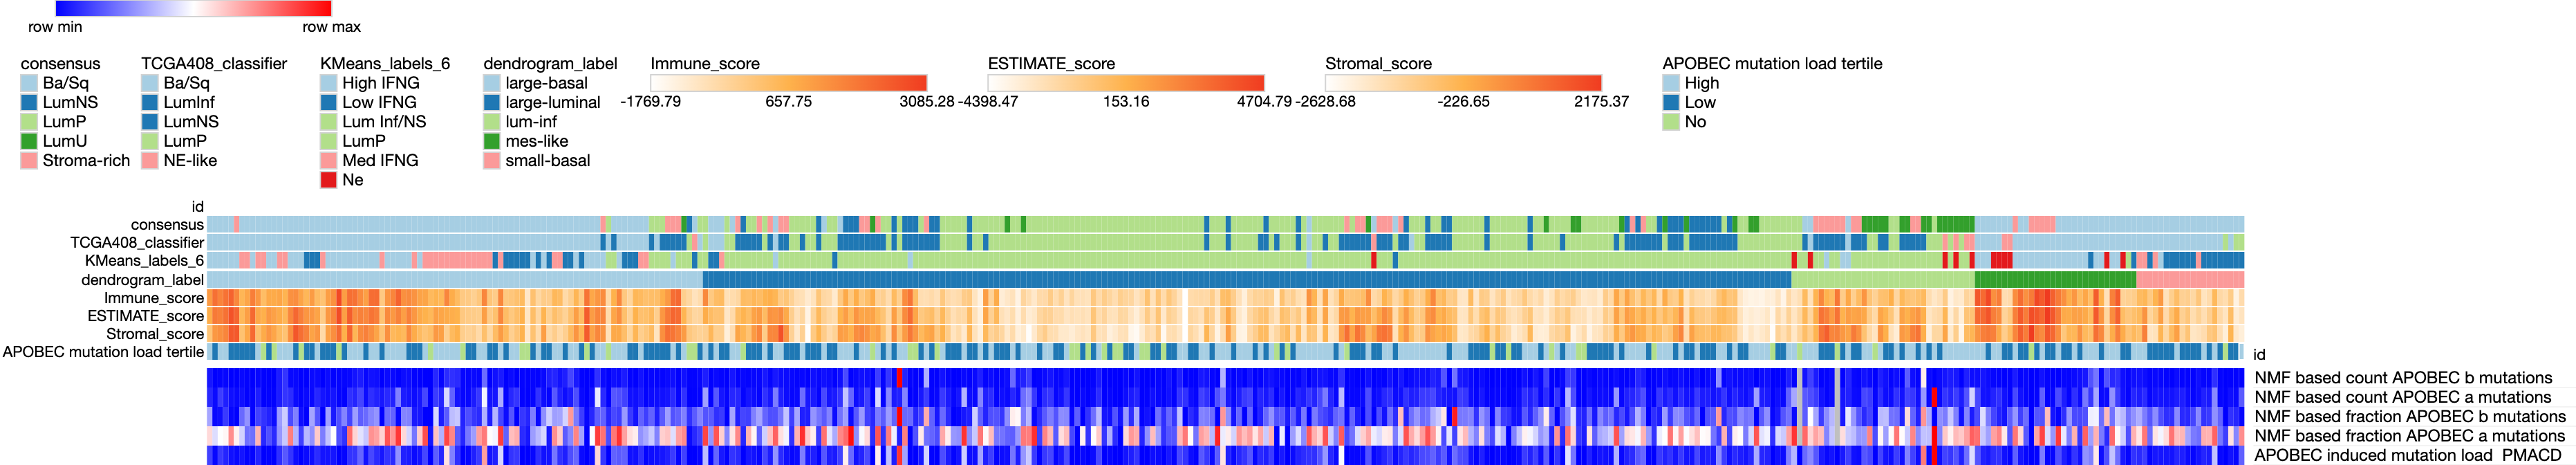
\includegraphics[width=1.0\textwidth,keepaspectratio]{Sections/Network_I/Resources/selective_pruning/sel_tfs/sel_tfs_apobec_meta.png}
      \caption{Heatmap of the the APOBEC mutations in TCGA.}
    \label{fig:ap:sel_tfs_tcga_meta_apobec}
\end{figure}

\newpage 

% TCGA somatic mutations
\section{TCGA somatic mutation} \label{s:ap:sel_prun_mut}

\begin{figure}[!htb]   
    \centering
    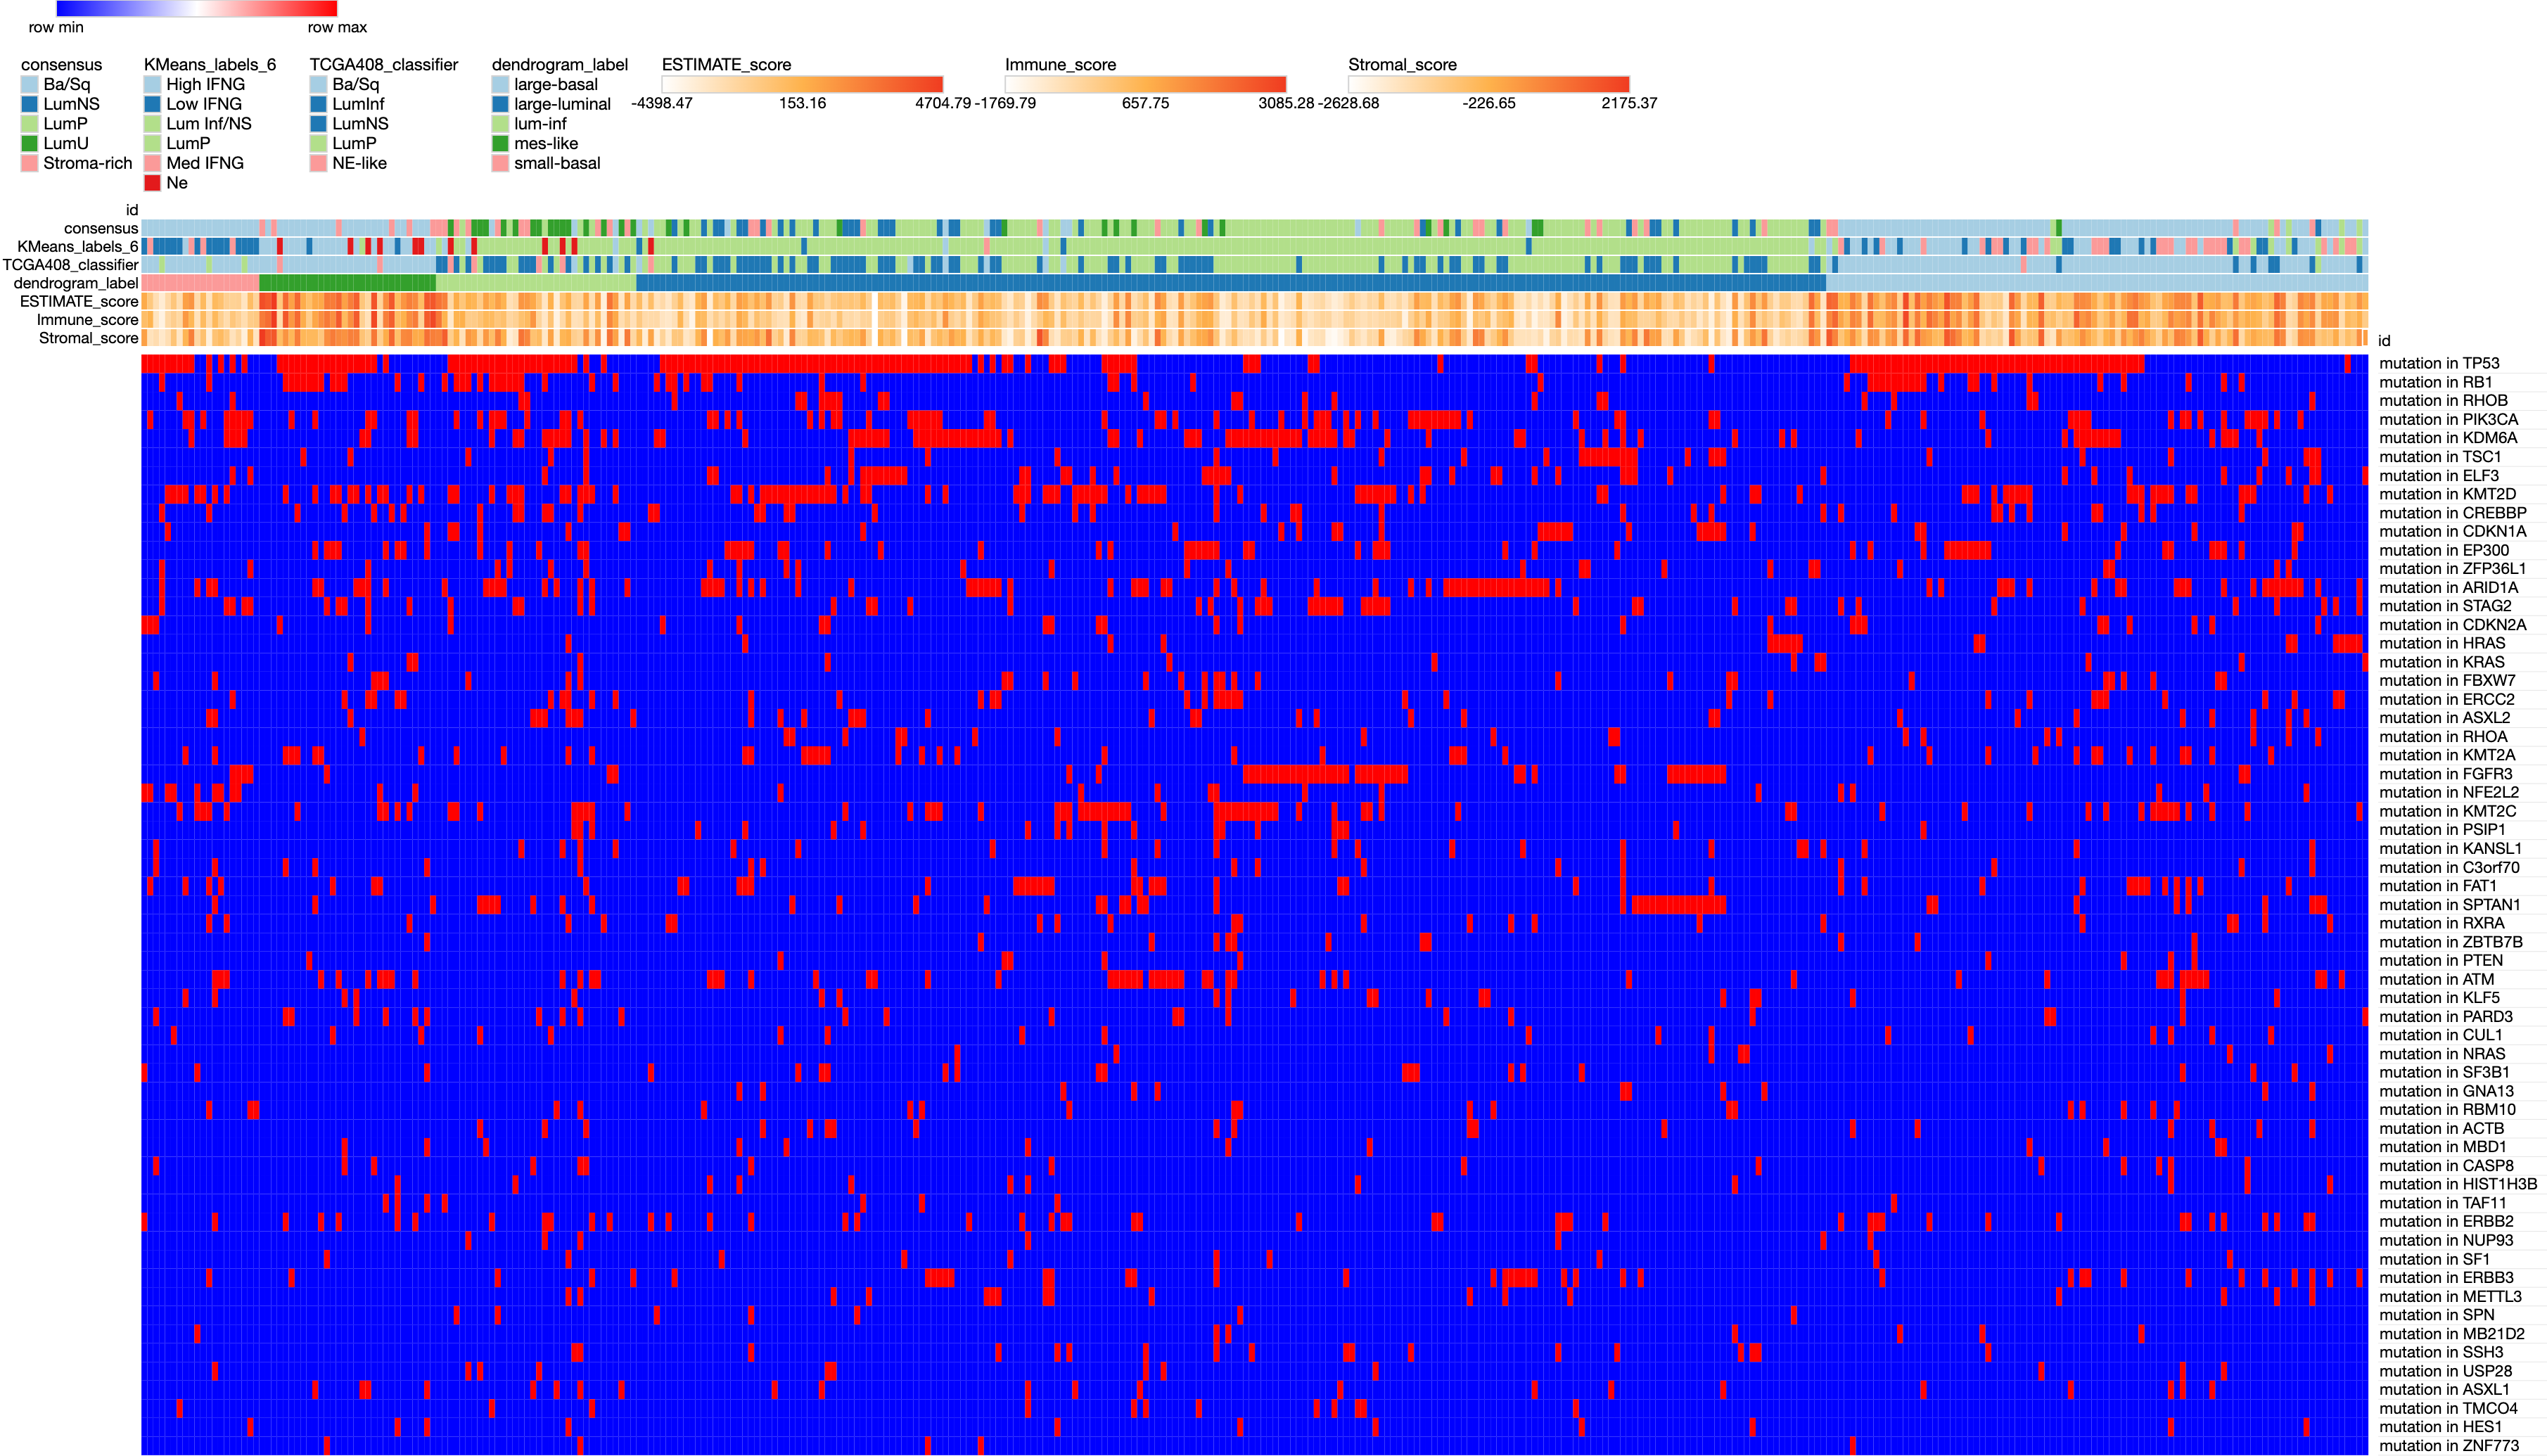
\includegraphics[width=1.0\textwidth,height=1.0\textheight,keepaspectratio]{Sections/Network_I/Resources/selective_pruning/sel_tfs/sel_tfs_mut_meta.png}
      \caption{Heatmap of binary somatic mutation across.}
    \label{fig:ap:sel_tfs_tcga_meta_mut}
\end{figure}

\newpage

% Pi-plots for GSEA
\section{Pi-plots for GSEA} \label{s:ap:sel_prun_pi}


\begin{figure}[H]
    \centering
    \begin{subfigure}[!t]{1.0\linewidth}
        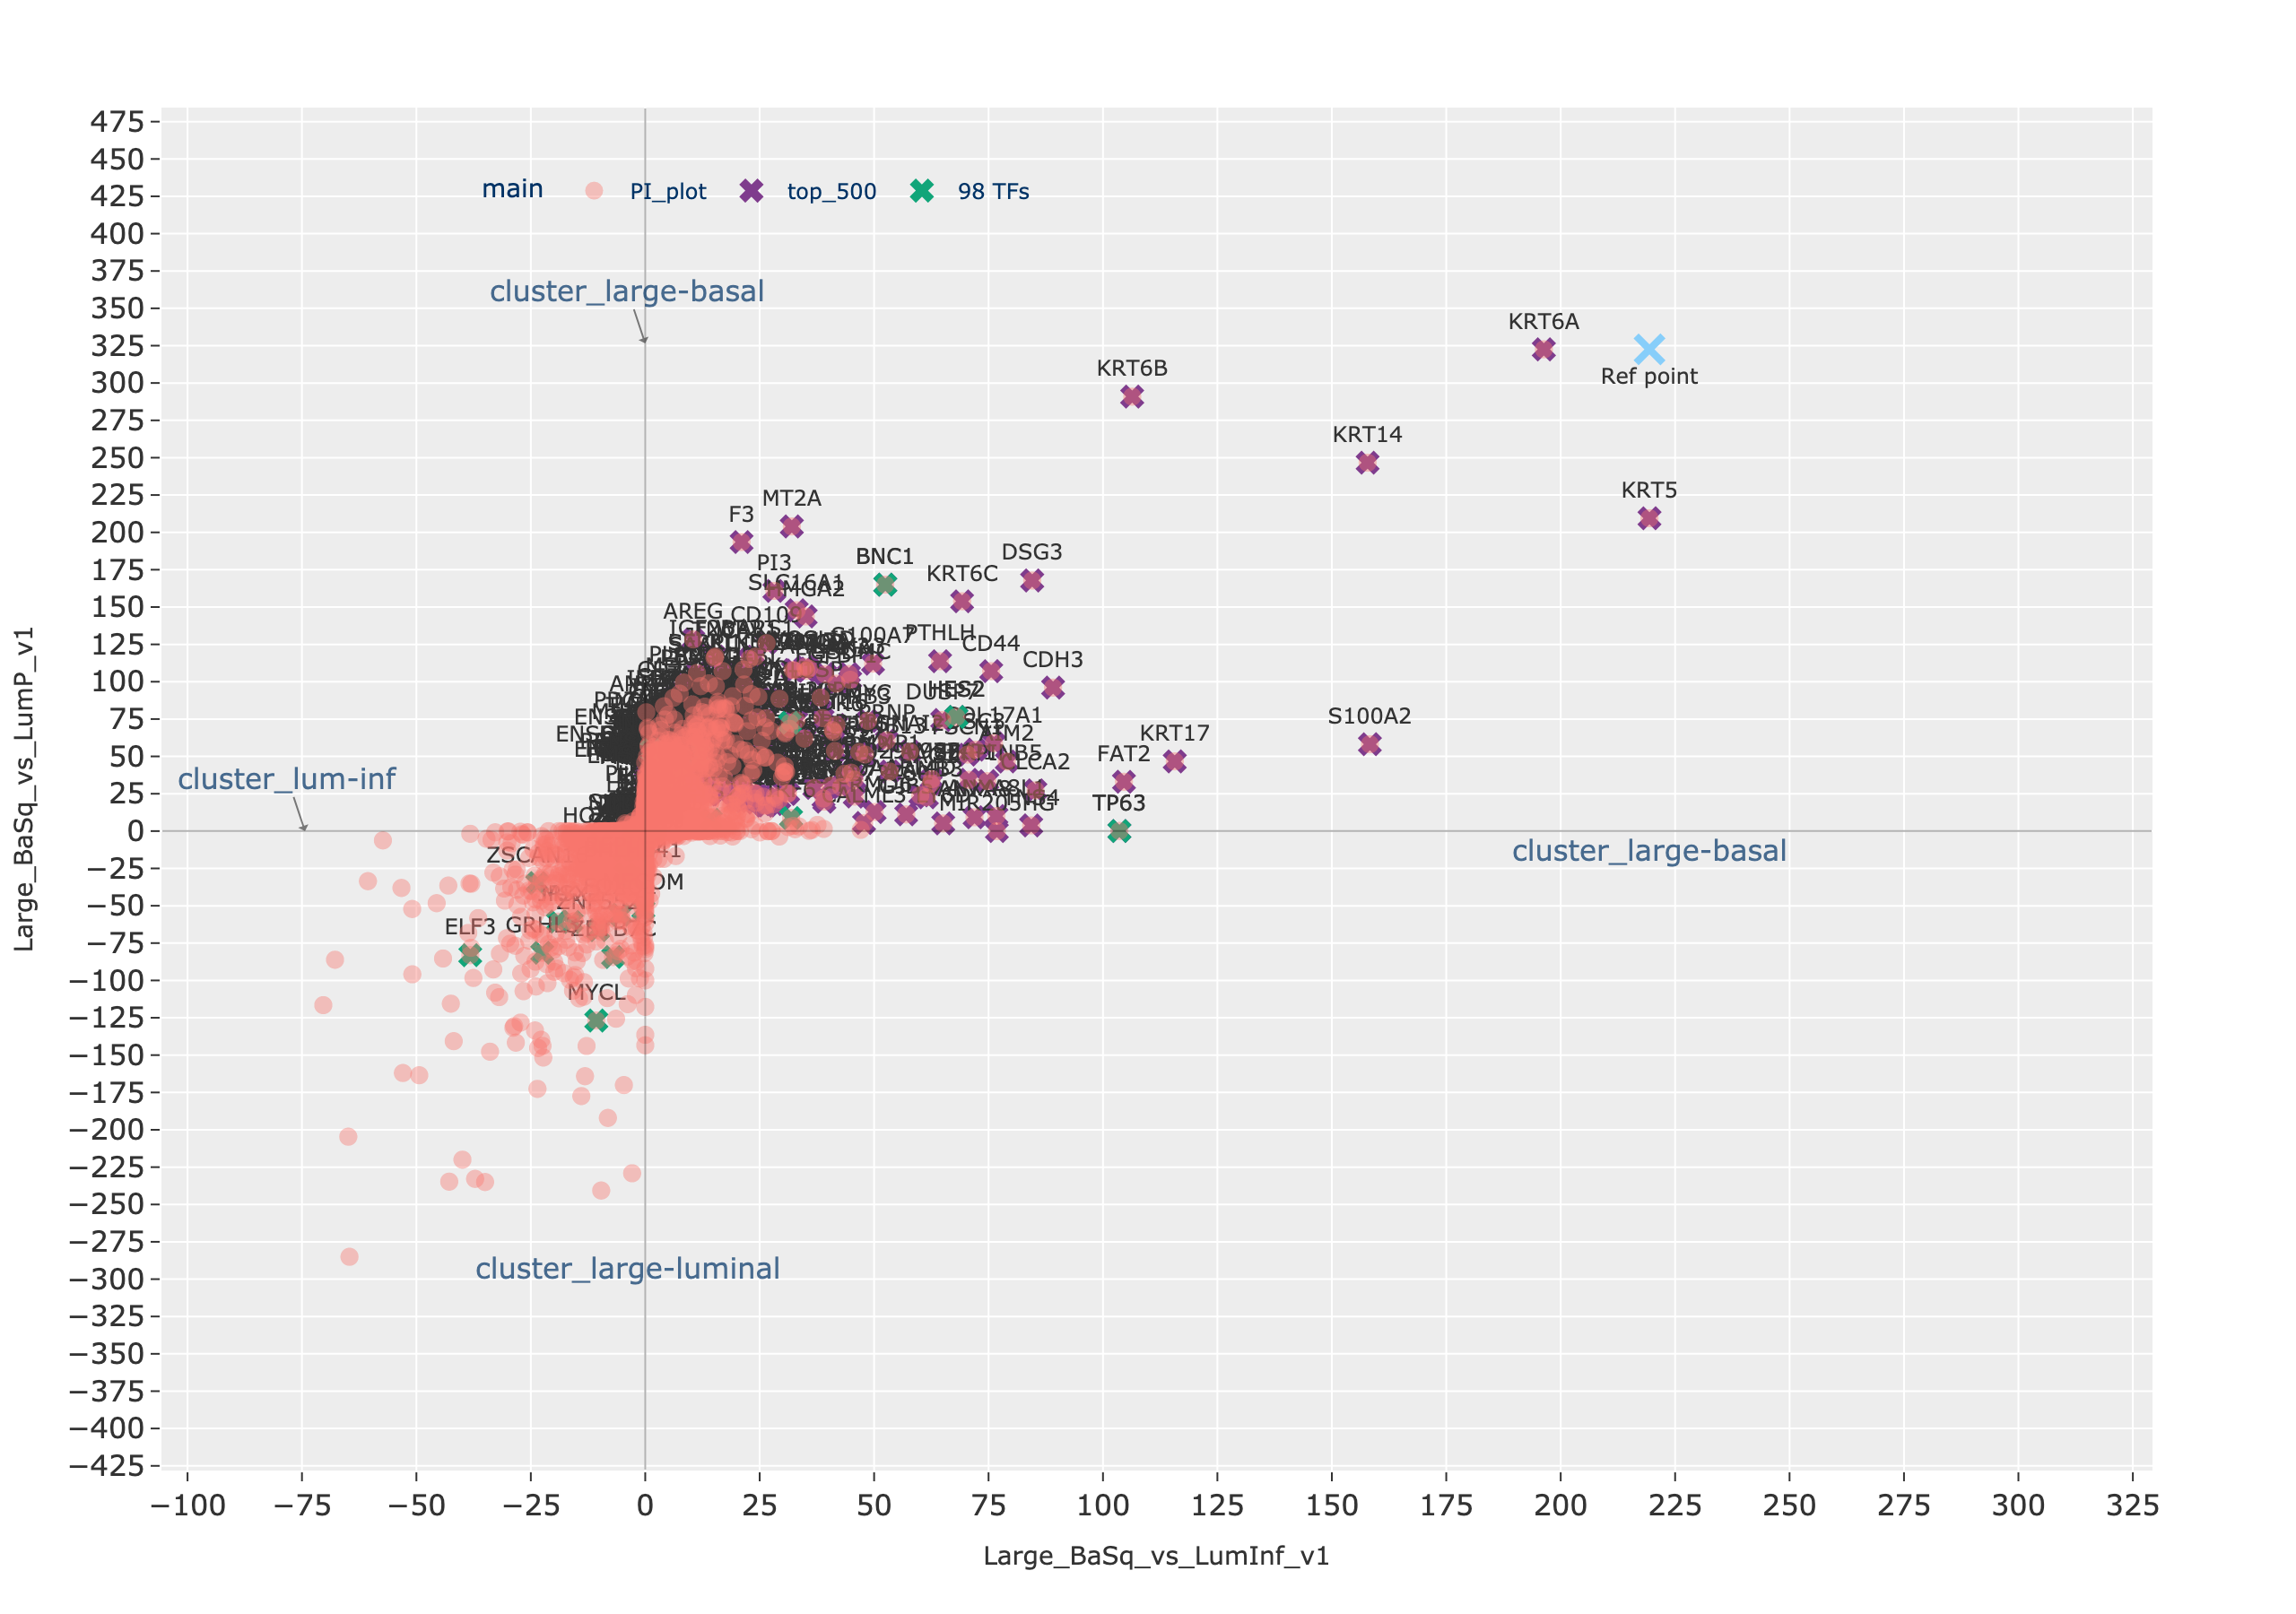
\includegraphics[width=\textwidth,keepaspectratio]{Sections/Network_I/Resources/selective_pruning/pi_gsea/pi_largeBasal.png}
        \caption{Large Basal}
        \label{fig:ap:pi_basal}
    \end{subfigure}
    \begin{subfigure}[!t]{1.0\textwidth}
        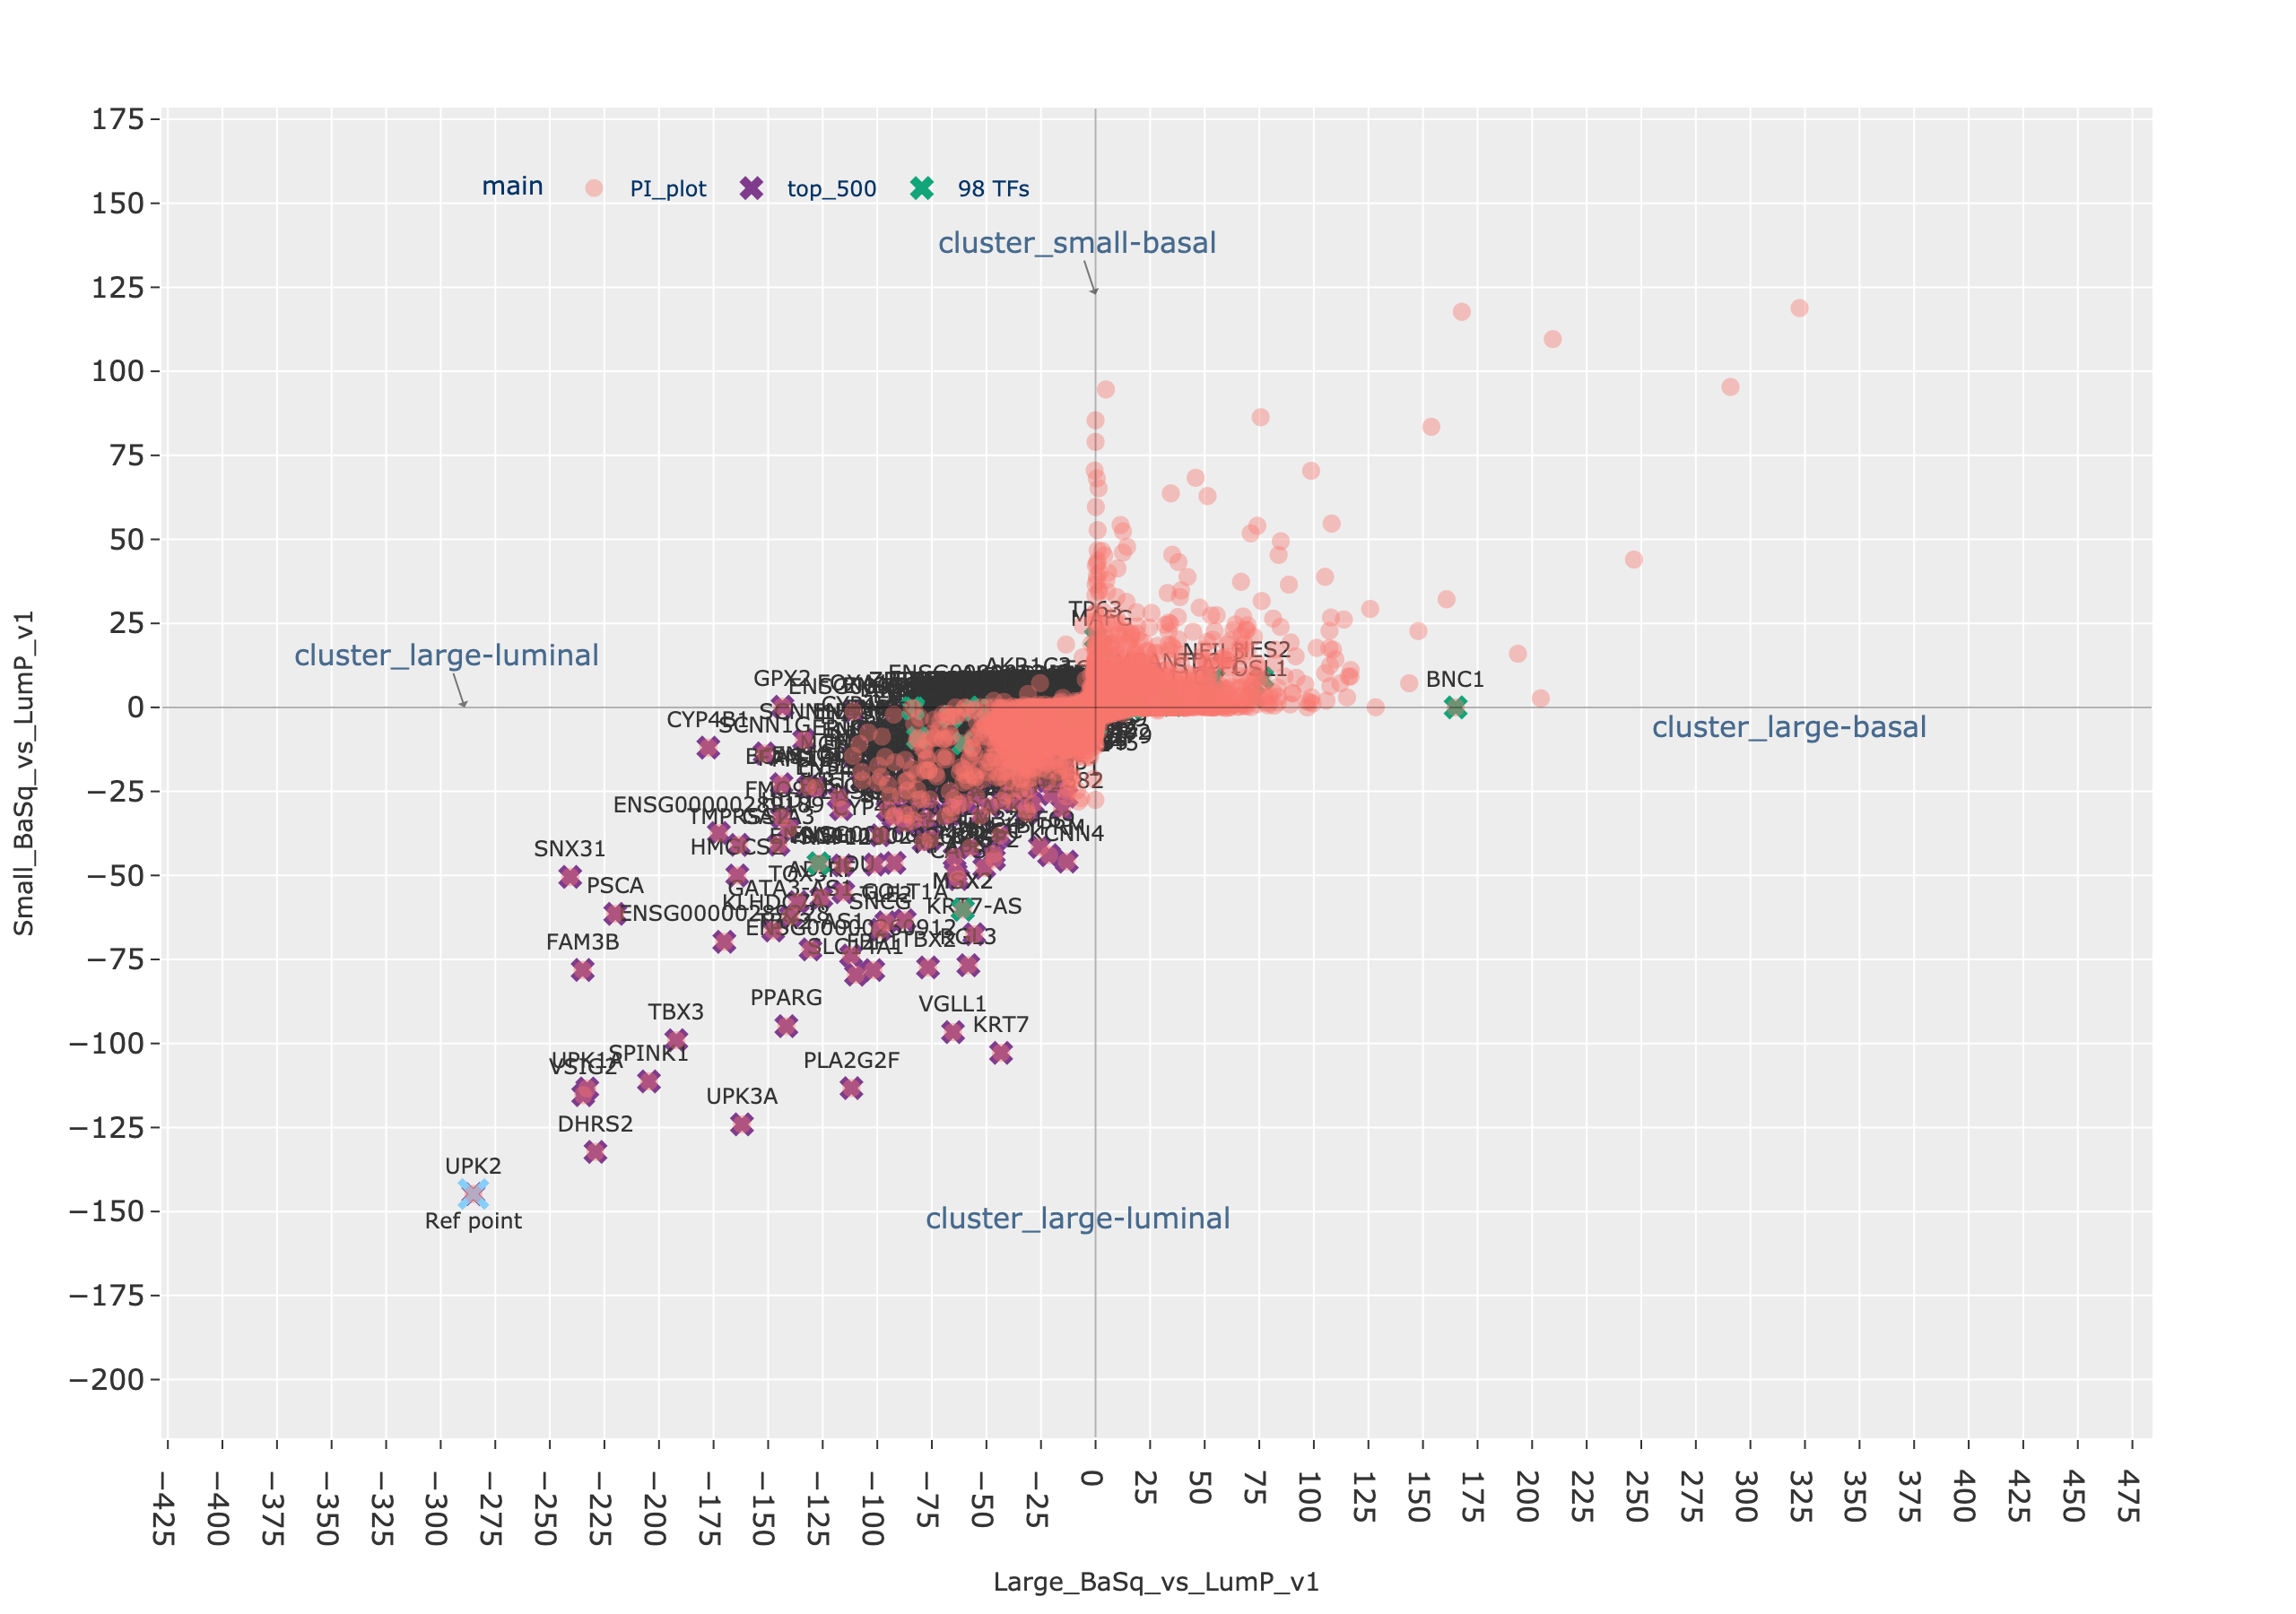
\includegraphics[width=\textwidth,keepaspectratio]{Sections/Network_I/Resources/selective_pruning/pi_gsea/pi_largeLuminal.png}
        \caption{Large luminal}
        \label{fig:ap:pi_lum}
    \end{subfigure}
    \caption{Pi plots for mes-like and lumInf from \cref{s:N_I:sel_tfs_subtypes}}
    \label{fig:ap:pi_other_values_I}
\end{figure}

\begin{figure}[!h]
    \centering
    \begin{subfigure}[!t]{1.0\textwidth}
        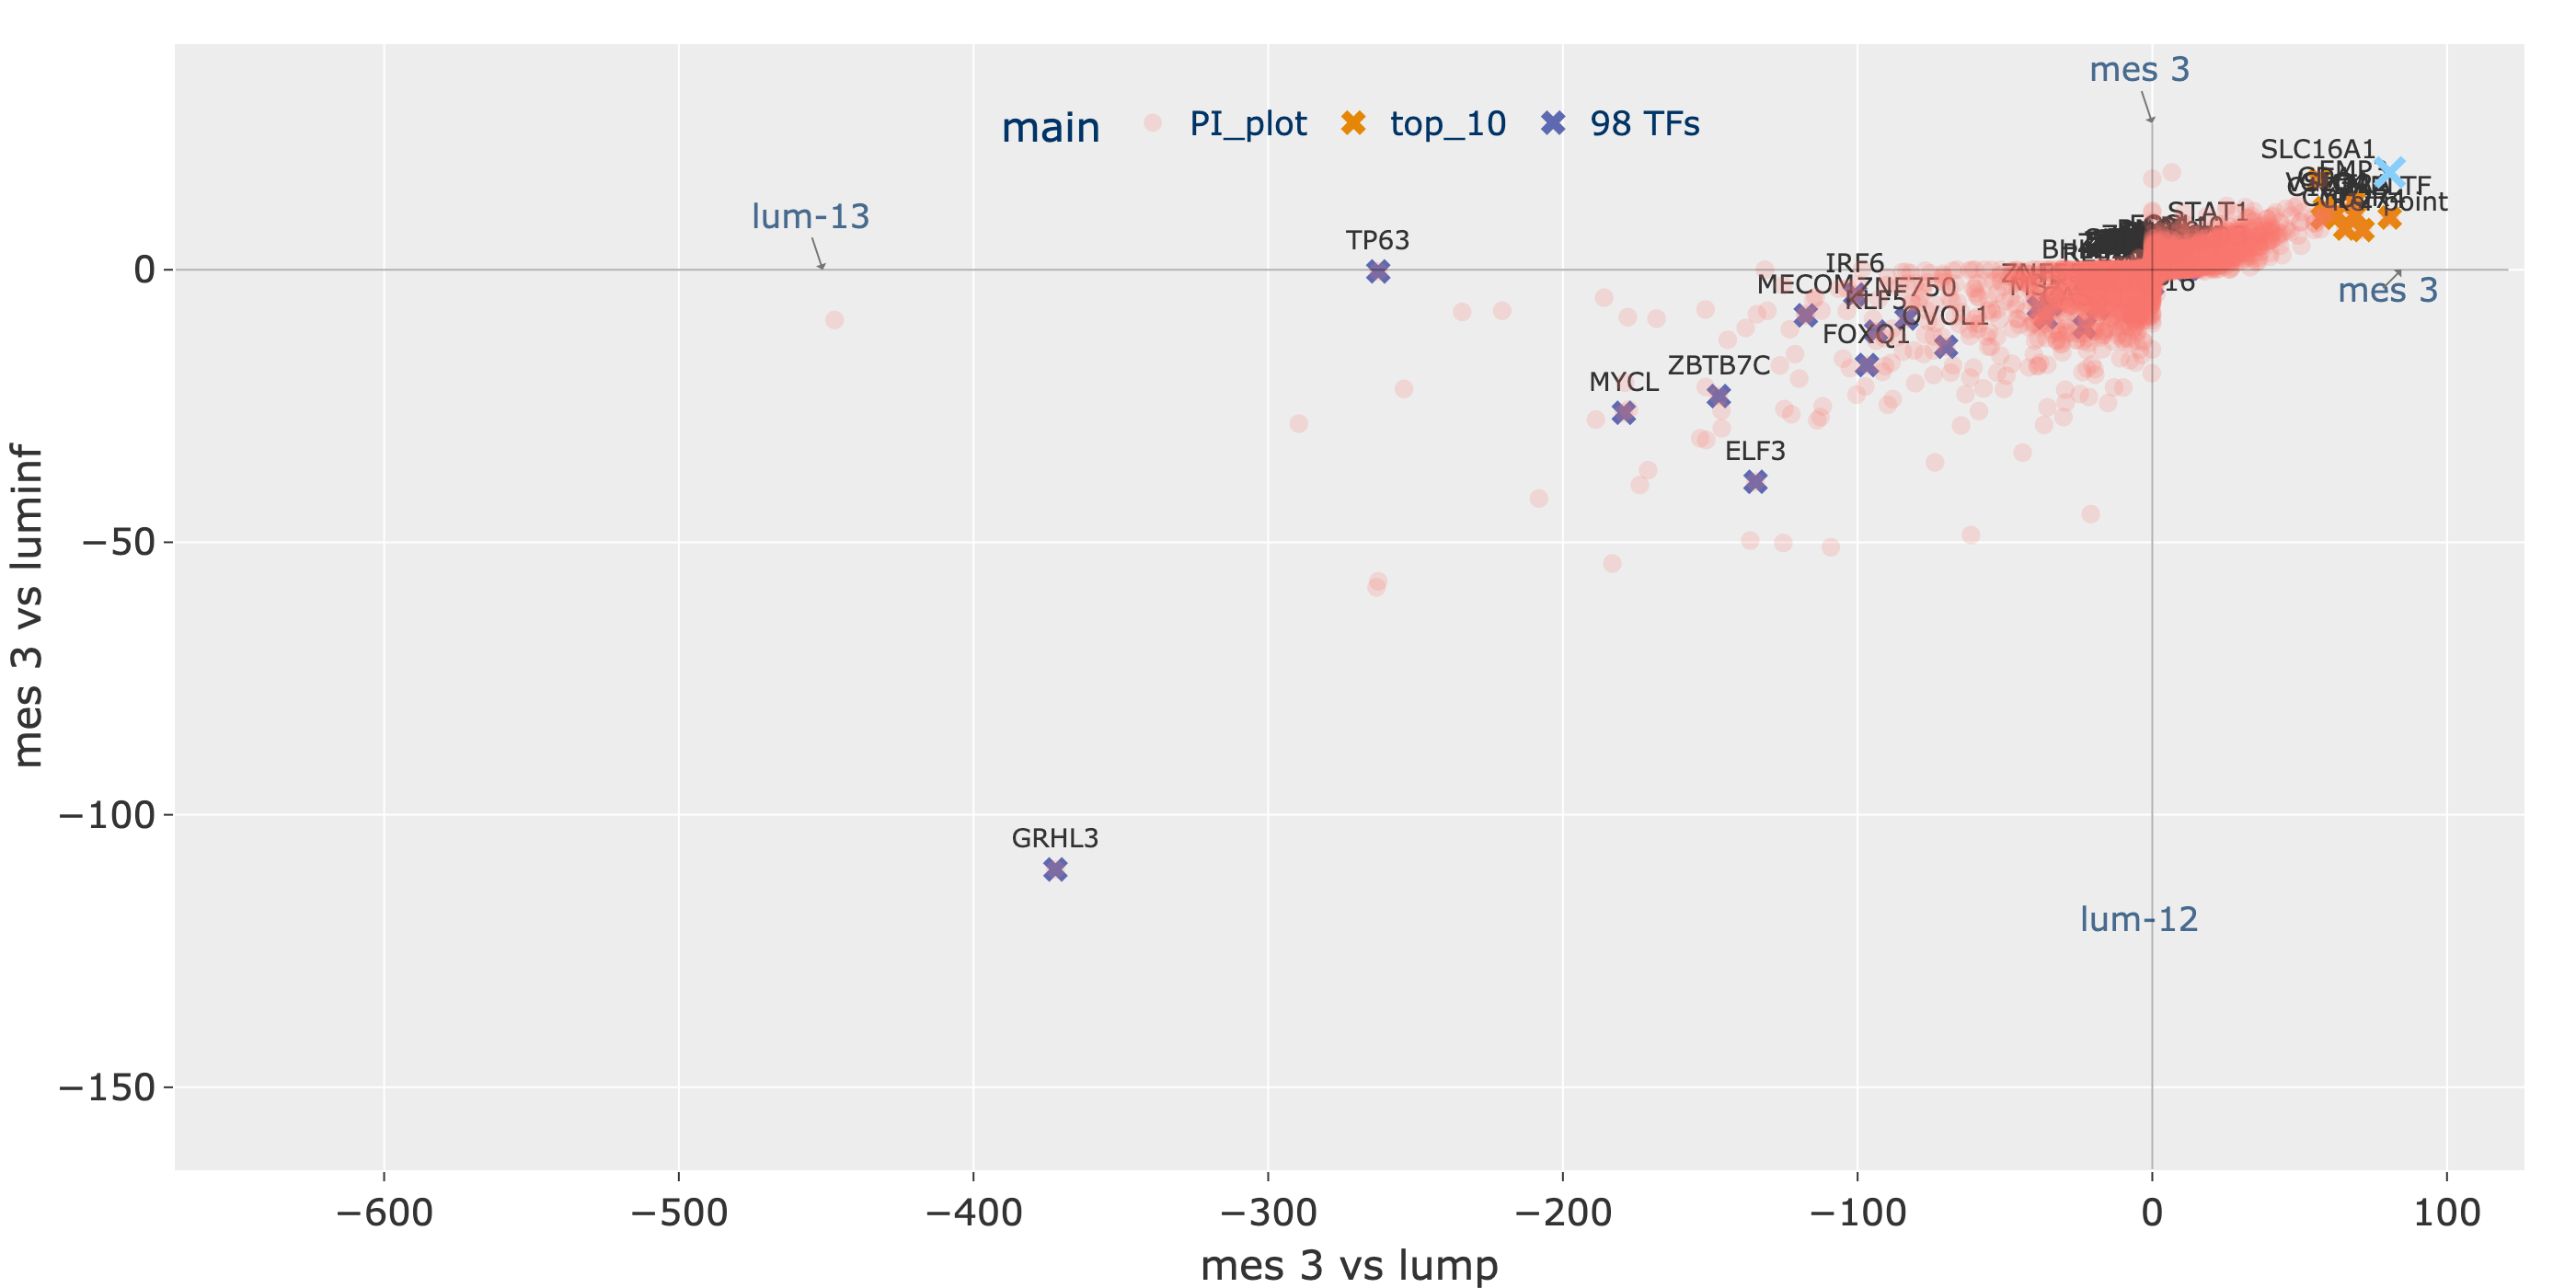
\includegraphics[width=\textwidth,keepaspectratio]{Sections/Network_I/Resources/selective_pruning/pi_gsea/pi_mesLike.png}
        \caption{Mes-like}
        \label{fig:ap:mes_like}
    \end{subfigure}
    \begin{subfigure}[!t]{1.0\textwidth}
        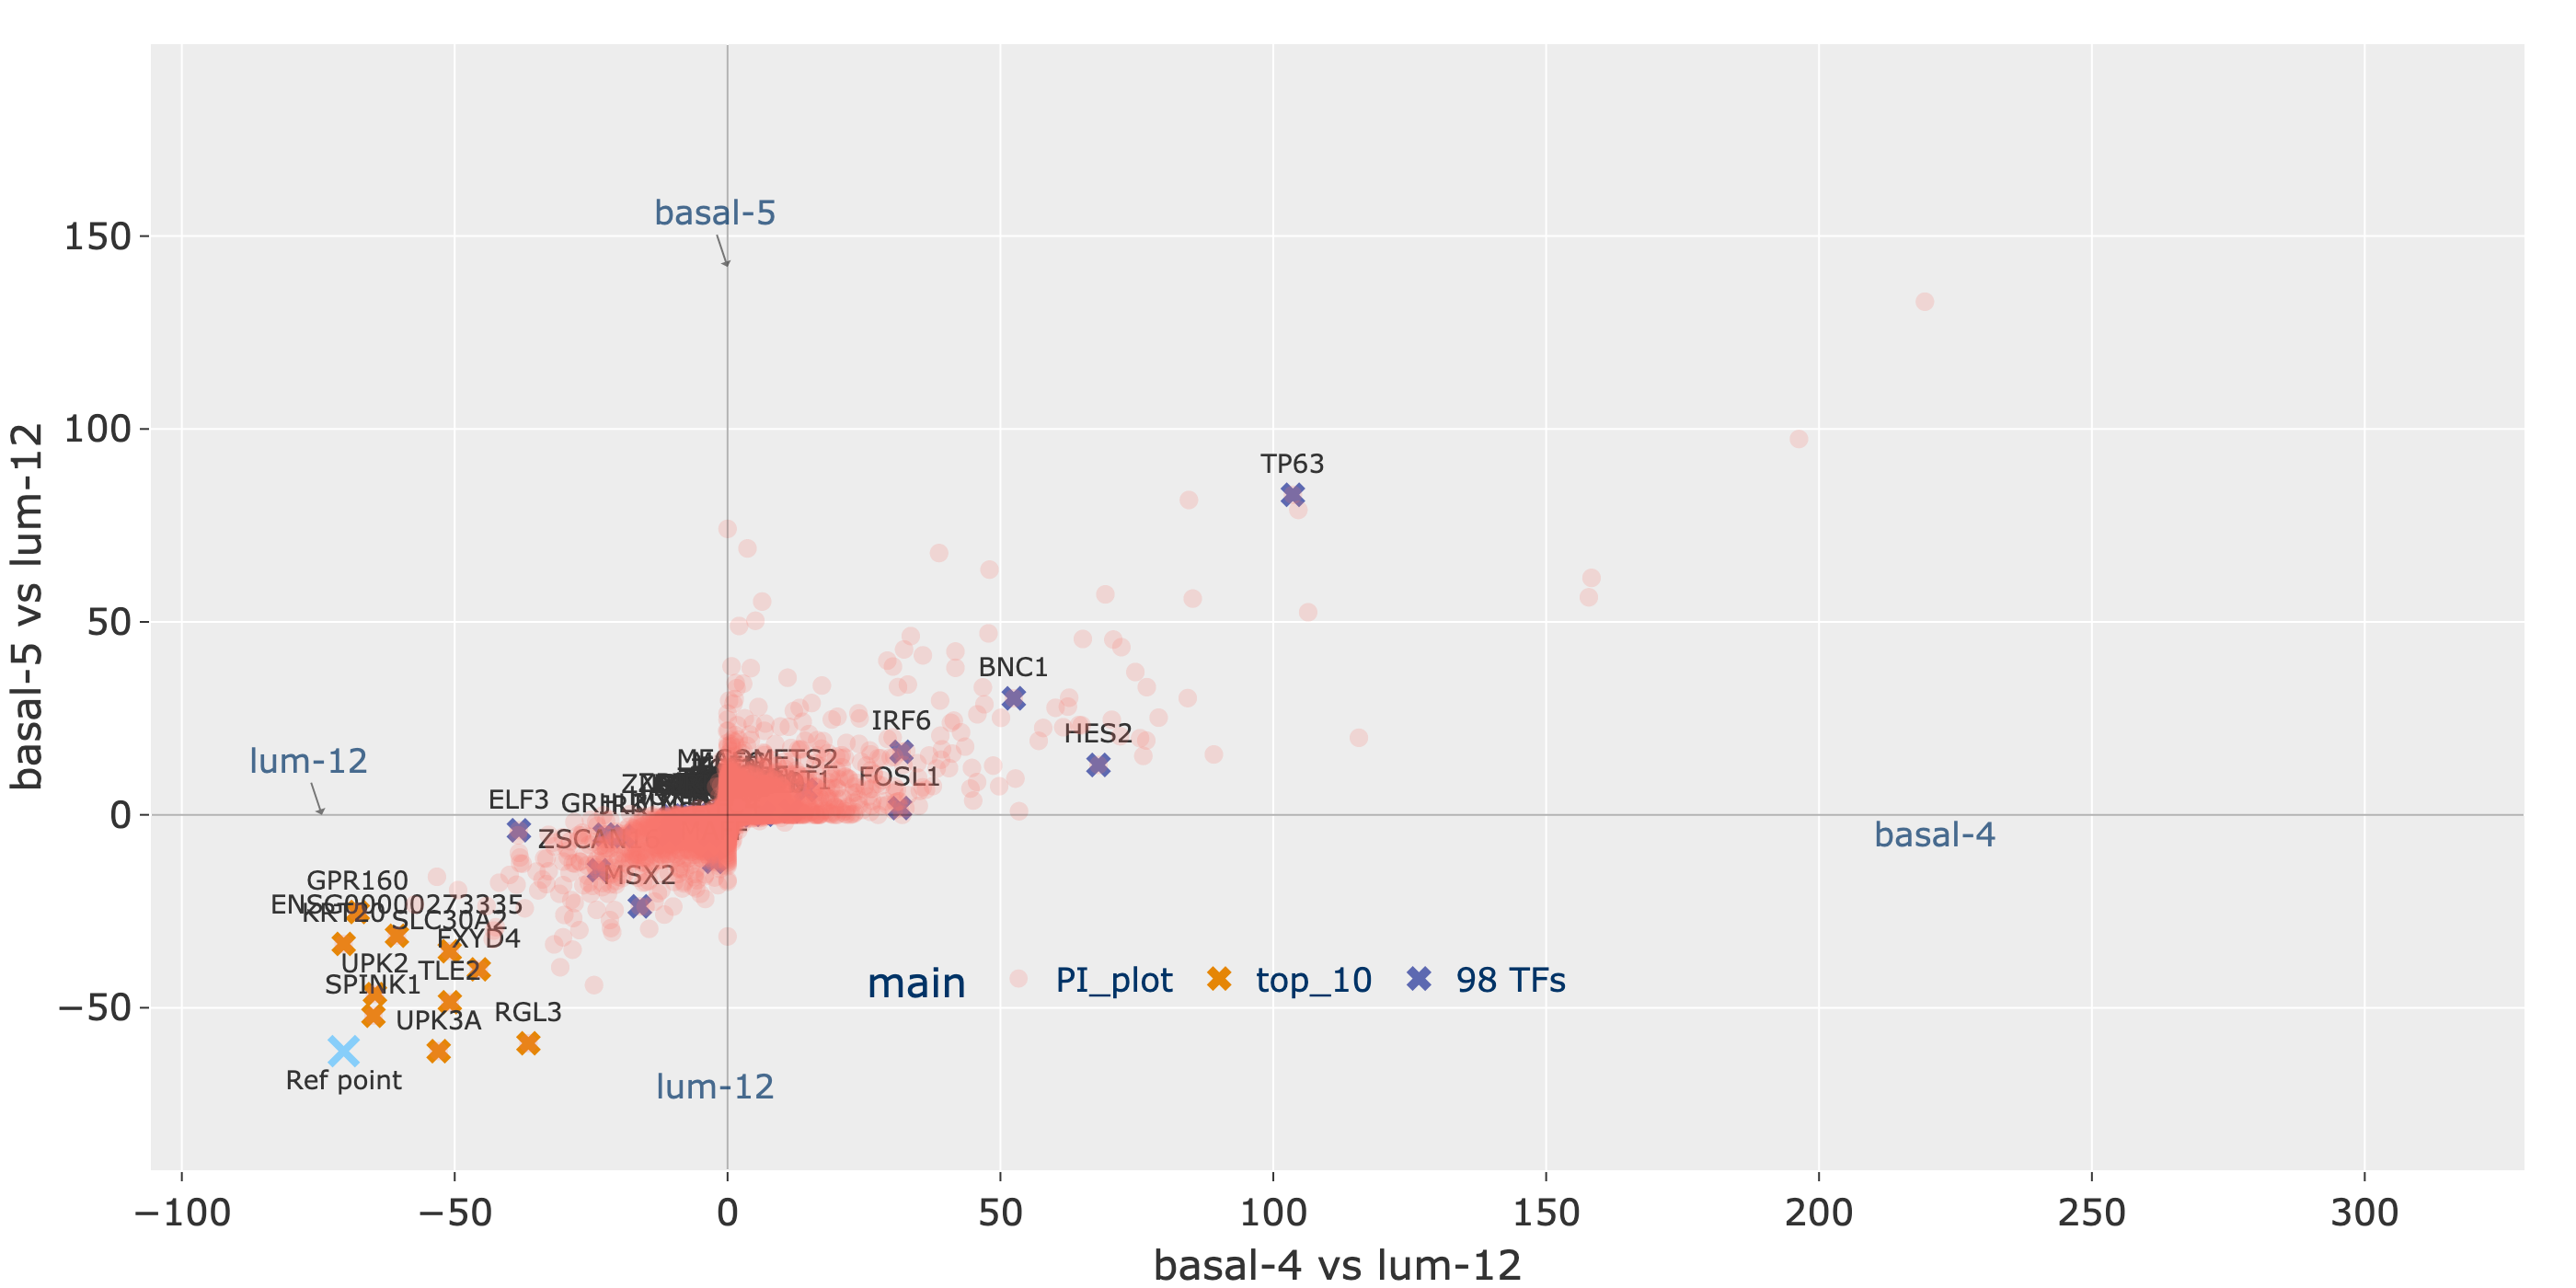
\includegraphics[width=\textwidth,keepaspectratio]{Sections/Network_I/Resources/selective_pruning/pi_gsea/pi_lumInf.png}
        \caption{Luminal infiltrated}
        \label{fig:ap:lumInf}
    \end{subfigure} 
    \caption{Pi plots for mes-like and lumInf from \cref{s:N_I:sel_tfs_subtypes}}
    \label{fig:ap:pi_other_values_II}
\end{figure}

\newpage

% GSEA - hallmarks
\section{GSEA output (Hallmarks)} \label{s:ap:hallmarks}

\begin{table}[H]
  \centering
  \scriptsize
  \begin{tabularx}{\textwidth}{>{\hsize=1.5\hsize}X|>{\hsize=0.4\hsize}X|>{\hsize=0.4\hsize}X|>{\hsize=0.6\hsize}X|>{\hsize=0.4\hsize}X|>{\hsize=0.4\hsize}X}
    \toprule
    \textbf{Term} & \textbf{NES} & \textbf{FDR q-val} & \textbf{\# lead} & \textbf{\# matched} & \textbf{ratio} \\
    \midrule
    \multicolumn{6}{c}{\textbf{smallBasal}} \\
    \midrule
    MYC TARGETS V1 & 1.909 & 0 & 149 & 40 & 0.268 \\
    \midrule
    MITOTIC SPINDLE & 1.887 & 0 & 138 & 61 & 0.442 \\
    \midrule
    TGF BETA SIGNALING & 1.863 & 0 & 28 & 15 & 0.536 \\
    \midrule
    \multicolumn{6}{c}{\textbf{largeBasal}} \\
    \midrule
    KRAS SIGNALING UP & 2.384 & 0 & 132 & 104 & 0.788 \\
    \midrule
    \multicolumn{6}{c}{\textbf{lumInf}} \\
    \midrule
    CHOLESTEROL HOMEOSTASIS & 1.892 & 0 & 33 & 20 & 0.606 \\
    \midrule
    APOPTOSIS & 1.733 & 0 & 61 & 37 & 0.607 \\
    \midrule
    \multicolumn{6}{c}{\textbf{largeLuminal}} \\
    \midrule
    DNA REPAIR & 1.617 & 0.004 & 77 & 12 & 0.156 \\
    \midrule
    PEROXISOME & 1.608 & 0.003 & 57 & 22 & 0.386 \\
    \midrule
    FATTY ACID METABOLISM & 1.552 & 0.004 & 71 & 38 & 0.535 \\
    \midrule
    PROTEIN SECRETION & 1.549 & 0.003 & 42 & 11 & 0.262 \\
    \midrule
    BILE ACID METABOLISM & 1.46 & 0.008 & 59 & 19 & 0.322 \\
    \bottomrule
  \end{tabularx}
  \caption{Normalised Enrichment Score (NES), False Discovery Rate (FDR) q-val, and lead gene statistics for different subtypes. The lead genes from a pathway are selected by GSEAY based on when the NES reached its peak.}
  \label{ap:tab:gsea_hallmark}
\end{table}

\newpage

% GSEA - oncoSig
\section{GSEA output (OncoSig)} \label{s:ap:sel_prun_oncosig}

% Table for OnCoSig
\begin{table}[H]
  \centering
  \scriptsize
  \begin{tabularx}{\textwidth}{>{\hsize=1.5\hsize}X|>{\hsize=0.4\hsize}X|>{\hsize=0.4\hsize}X|>{\hsize=0.6\hsize}X|>{\hsize=0.4\hsize}X|>{\hsize=0.4\hsize}X}
    \toprule
    \textbf{Term} & \textbf{NES} & \textbf{FDR q-val} & \textbf{\# lead genes} & \textbf{\# matchedl} & \textbf{ratio matched} \\
    \midrule
    \multicolumn{6}{c}{\textbf{smallBasal}} \\
    \midrule
    SINGH KRAS DEPENDENCY SIGNATURE & 2.121 & 0 & 17 & 10 & 0.588 \\
    \midrule
    TBK1.DF DN & 2.105 & 0 & 206 & 132 & 0.641 \\
    \midrule
    EIF4E DN & 2.084 & 0 & 53 & 44 & 0.83 \\
    \midrule
    PGF UP.V1 UP & 2.002 & 0 & 111 & 67 & 0.604 \\
    \midrule
    ERBB2 UP.V1 DN & 1.877 & 0 & 110 & 67 & 0.609 \\
    \midrule
    GCNP SHH UP LATE.V1 UP & 1.863 & 0 & 120 & 52 & 0.433 \\
    \midrule
    P53 DN.V1 UP & 1.862 & 0 & 68 & 65 & 0.956 \\
    \midrule
    RB P130 DN.V1 DN & 1.862 & 0 & 82 & 52 & 0.634 \\
    \midrule
    \multicolumn{6}{c}{\textbf{largeBasal}} \\
    \midrule
    CSR LATE UP.V1 UP & 2.382 & 0 & 115 & 86 & 0.748 \\
    \midrule
    TBK1.DF UP & 2.332 & 0 & 173 & 135 & 0.78 \\
    \midrule
    CSR EARLY UP.V1 UP & 2.326 & 0 & 110 & 74 & 0.673 \\
    \midrule
    \multicolumn{6}{c}{\textbf{mesLike}} \\
    \midrule
    CORDENONSI YAP CONSERVED SIGNATURE & 2.49 & 0 & 48 & 39 & 0.812 \\
    \midrule
    LEF1 UP.V1 UP & 2.423 & 0 & 125 & 110 & 0.88 \\
    \midrule
    RB P107 DN.V1 UP & 2.316 & 0 & 84 & 71 & 0.845 \\
    \midrule
    LTE2 UP.V1 DN & 2.265 & 0 & 118 & 86 & 0.729 \\
    \midrule
    \multicolumn{6}{c}{\textbf{lumInf}} \\
    \midrule
    BCAT.100 UP.V1 UP & 2.067 & 0 & 24 & 22 & 0.917 \\
    \midrule
    CSR LATE UP.V1 DN & 1.964 & 0 & 70 & 49 & 0.7 \\
    \midrule
    AKT UP.V1 DN & 1.889 & 0 & 90 & 66 & 0.733 \\
    \midrule
    ESC J1 UP LATE.V1 UP & 1.828 & 0 & 81 & 67 & 0.827 \\
    \midrule
    \multicolumn{6}{c}{\textbf{largeLuminal}} \\
    CSR EARLY UP.V1 DN & 1.679 & 0.002 & 73 & 32 & 0.438 \\
    \midrule
    MYC UP.V1 DN & 1.613 & 0.002 & 77 & 38 & 0.494 \\
    \bottomrule
  \end{tabularx}
   \caption{Normalised Enrichment Score (NES), False Discovery Rate (FDR) q-val, and lead gene statistics for different subtypes and terms in bladder cancer biology from the OncoSig database. The lead genes from a pathway are selected by GSEAPY based on when the NES reached its peak.}
  \label{ap:tab:gsea_oncosig}
\end{table}

\newpage

% GSEA plots
\section{GSEA plots top 10 by Enrichment score}



\begin{figure}[!htb]
    \centering
    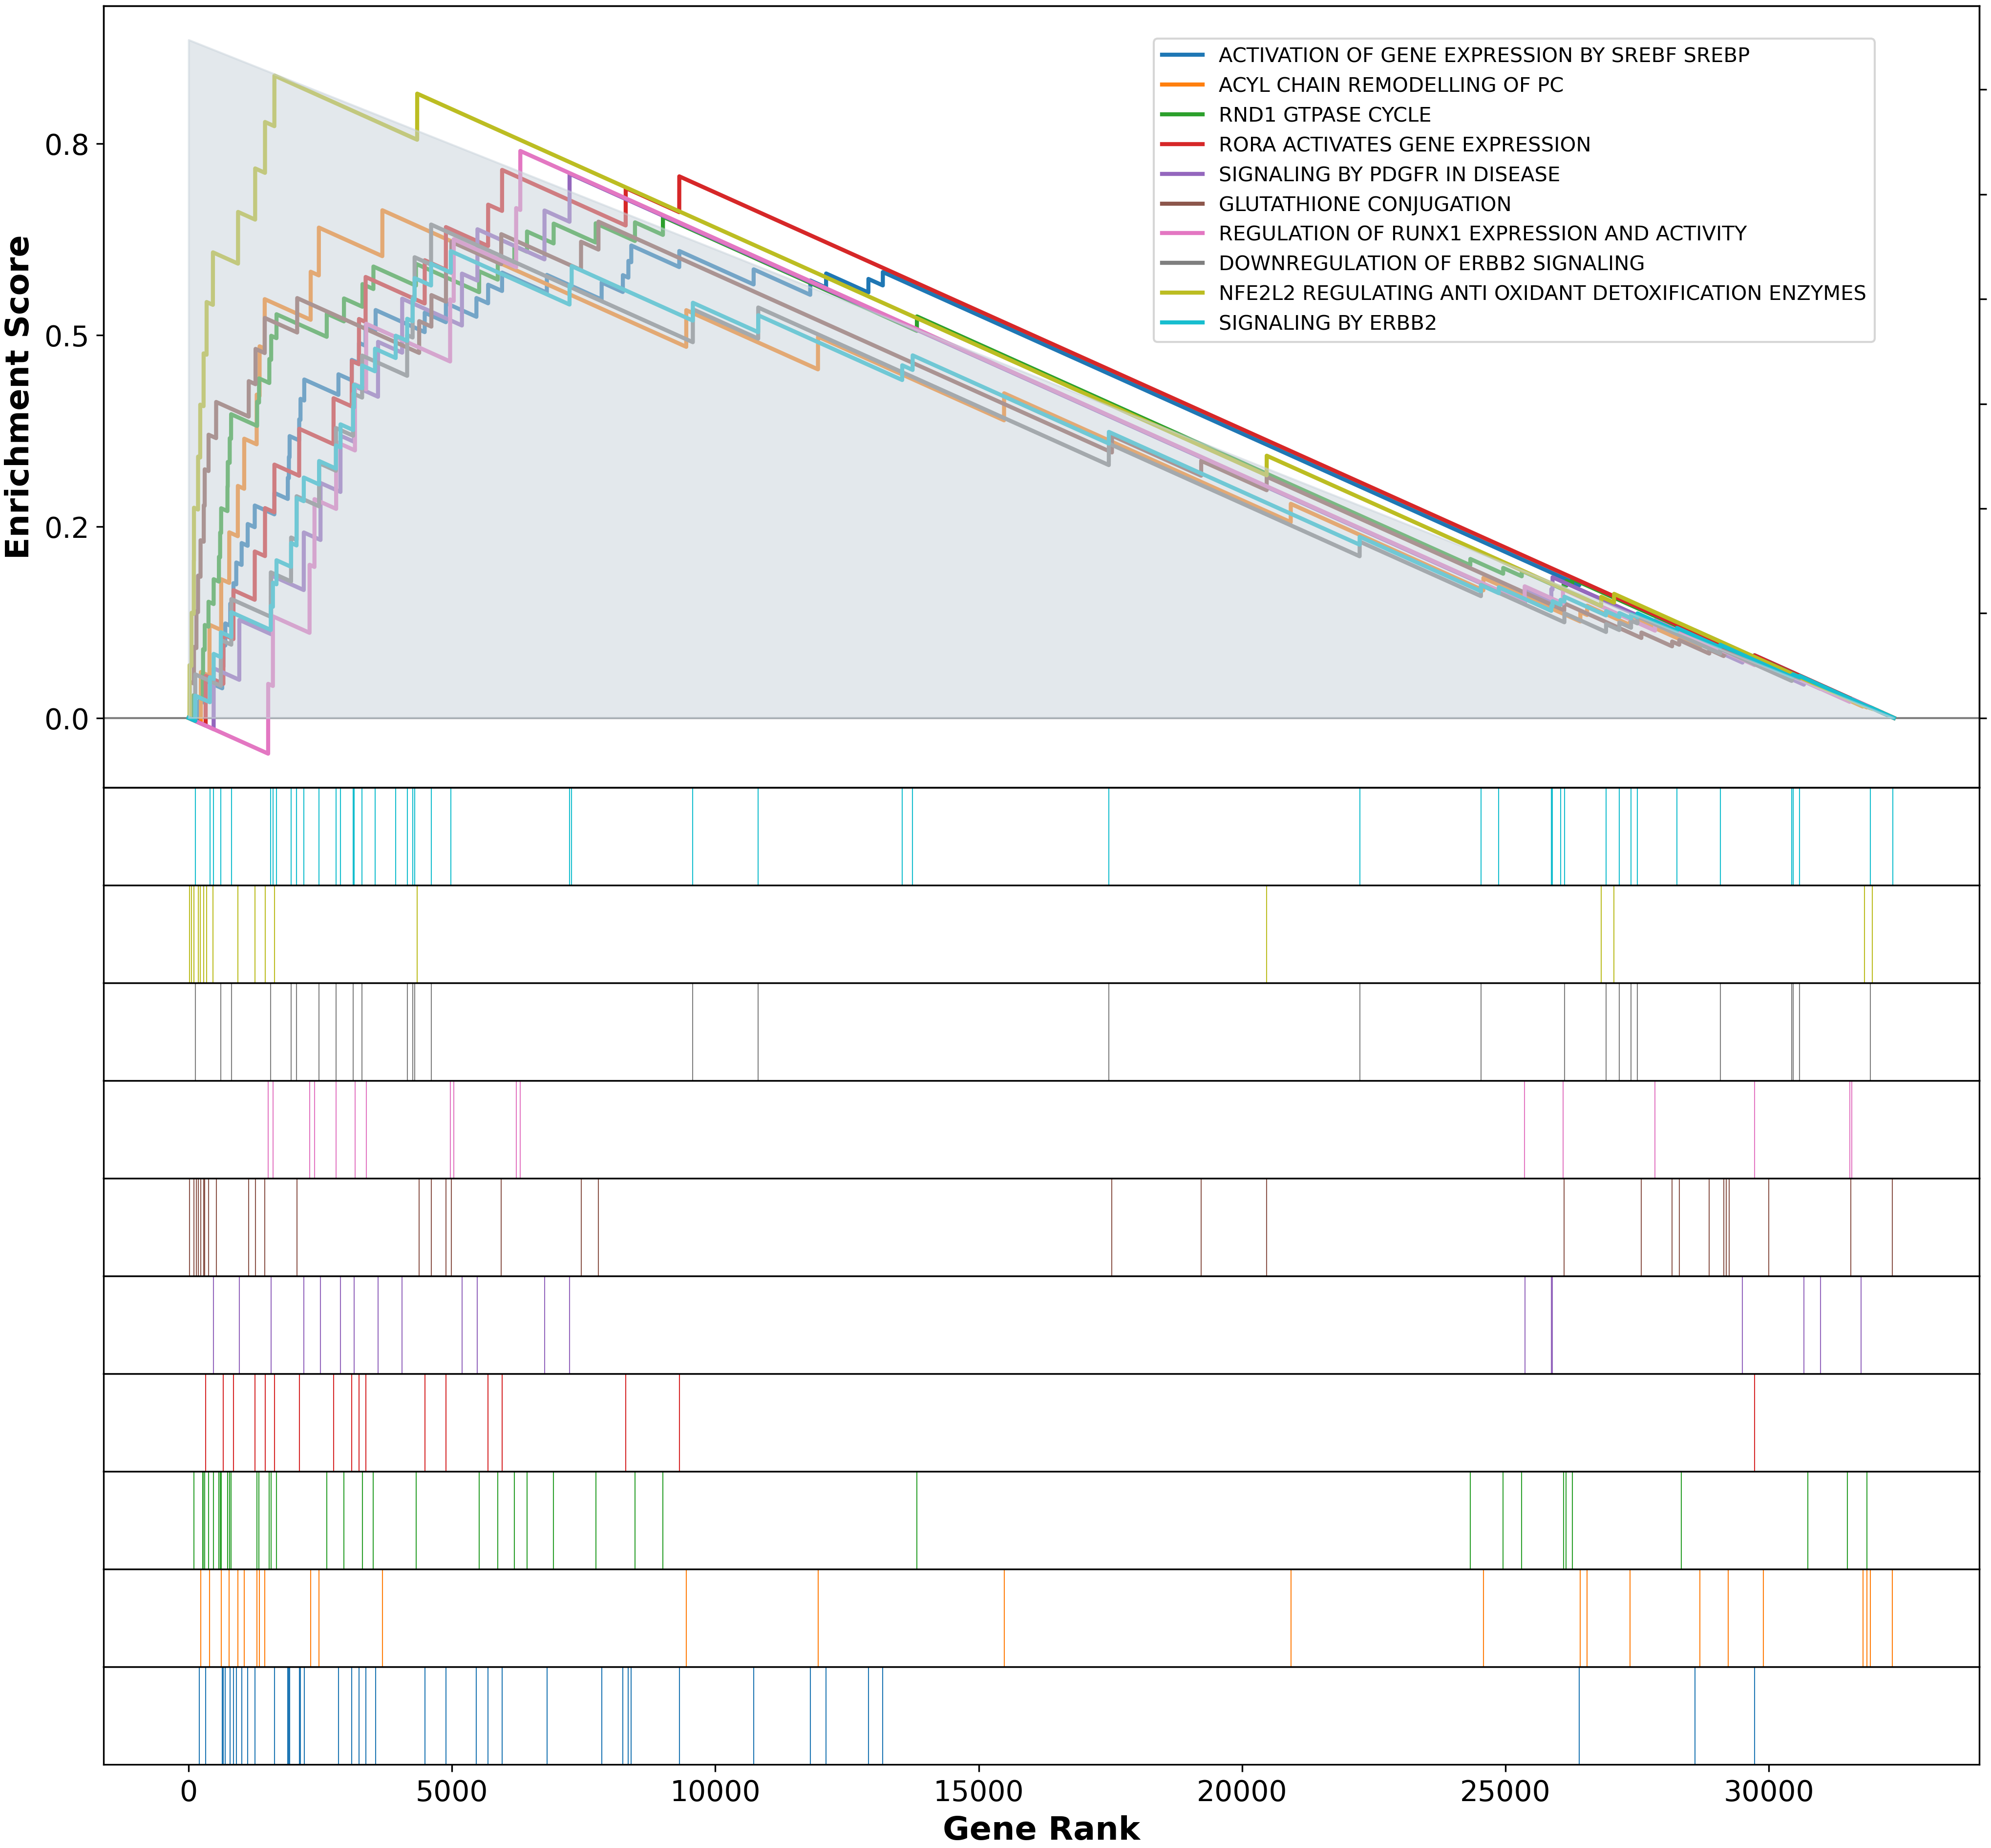
\includegraphics[width=\textwidth,keepaspectratio]{Sections/Network_I/Resources/selective_pruning/gsea/smallBasal_10_top_manTerms.png}
    \caption{Small Basal}
    \label{fig:ap:gsea_smallBasal}
\end{figure}


\begin{figure}[!htb]
    \centering
    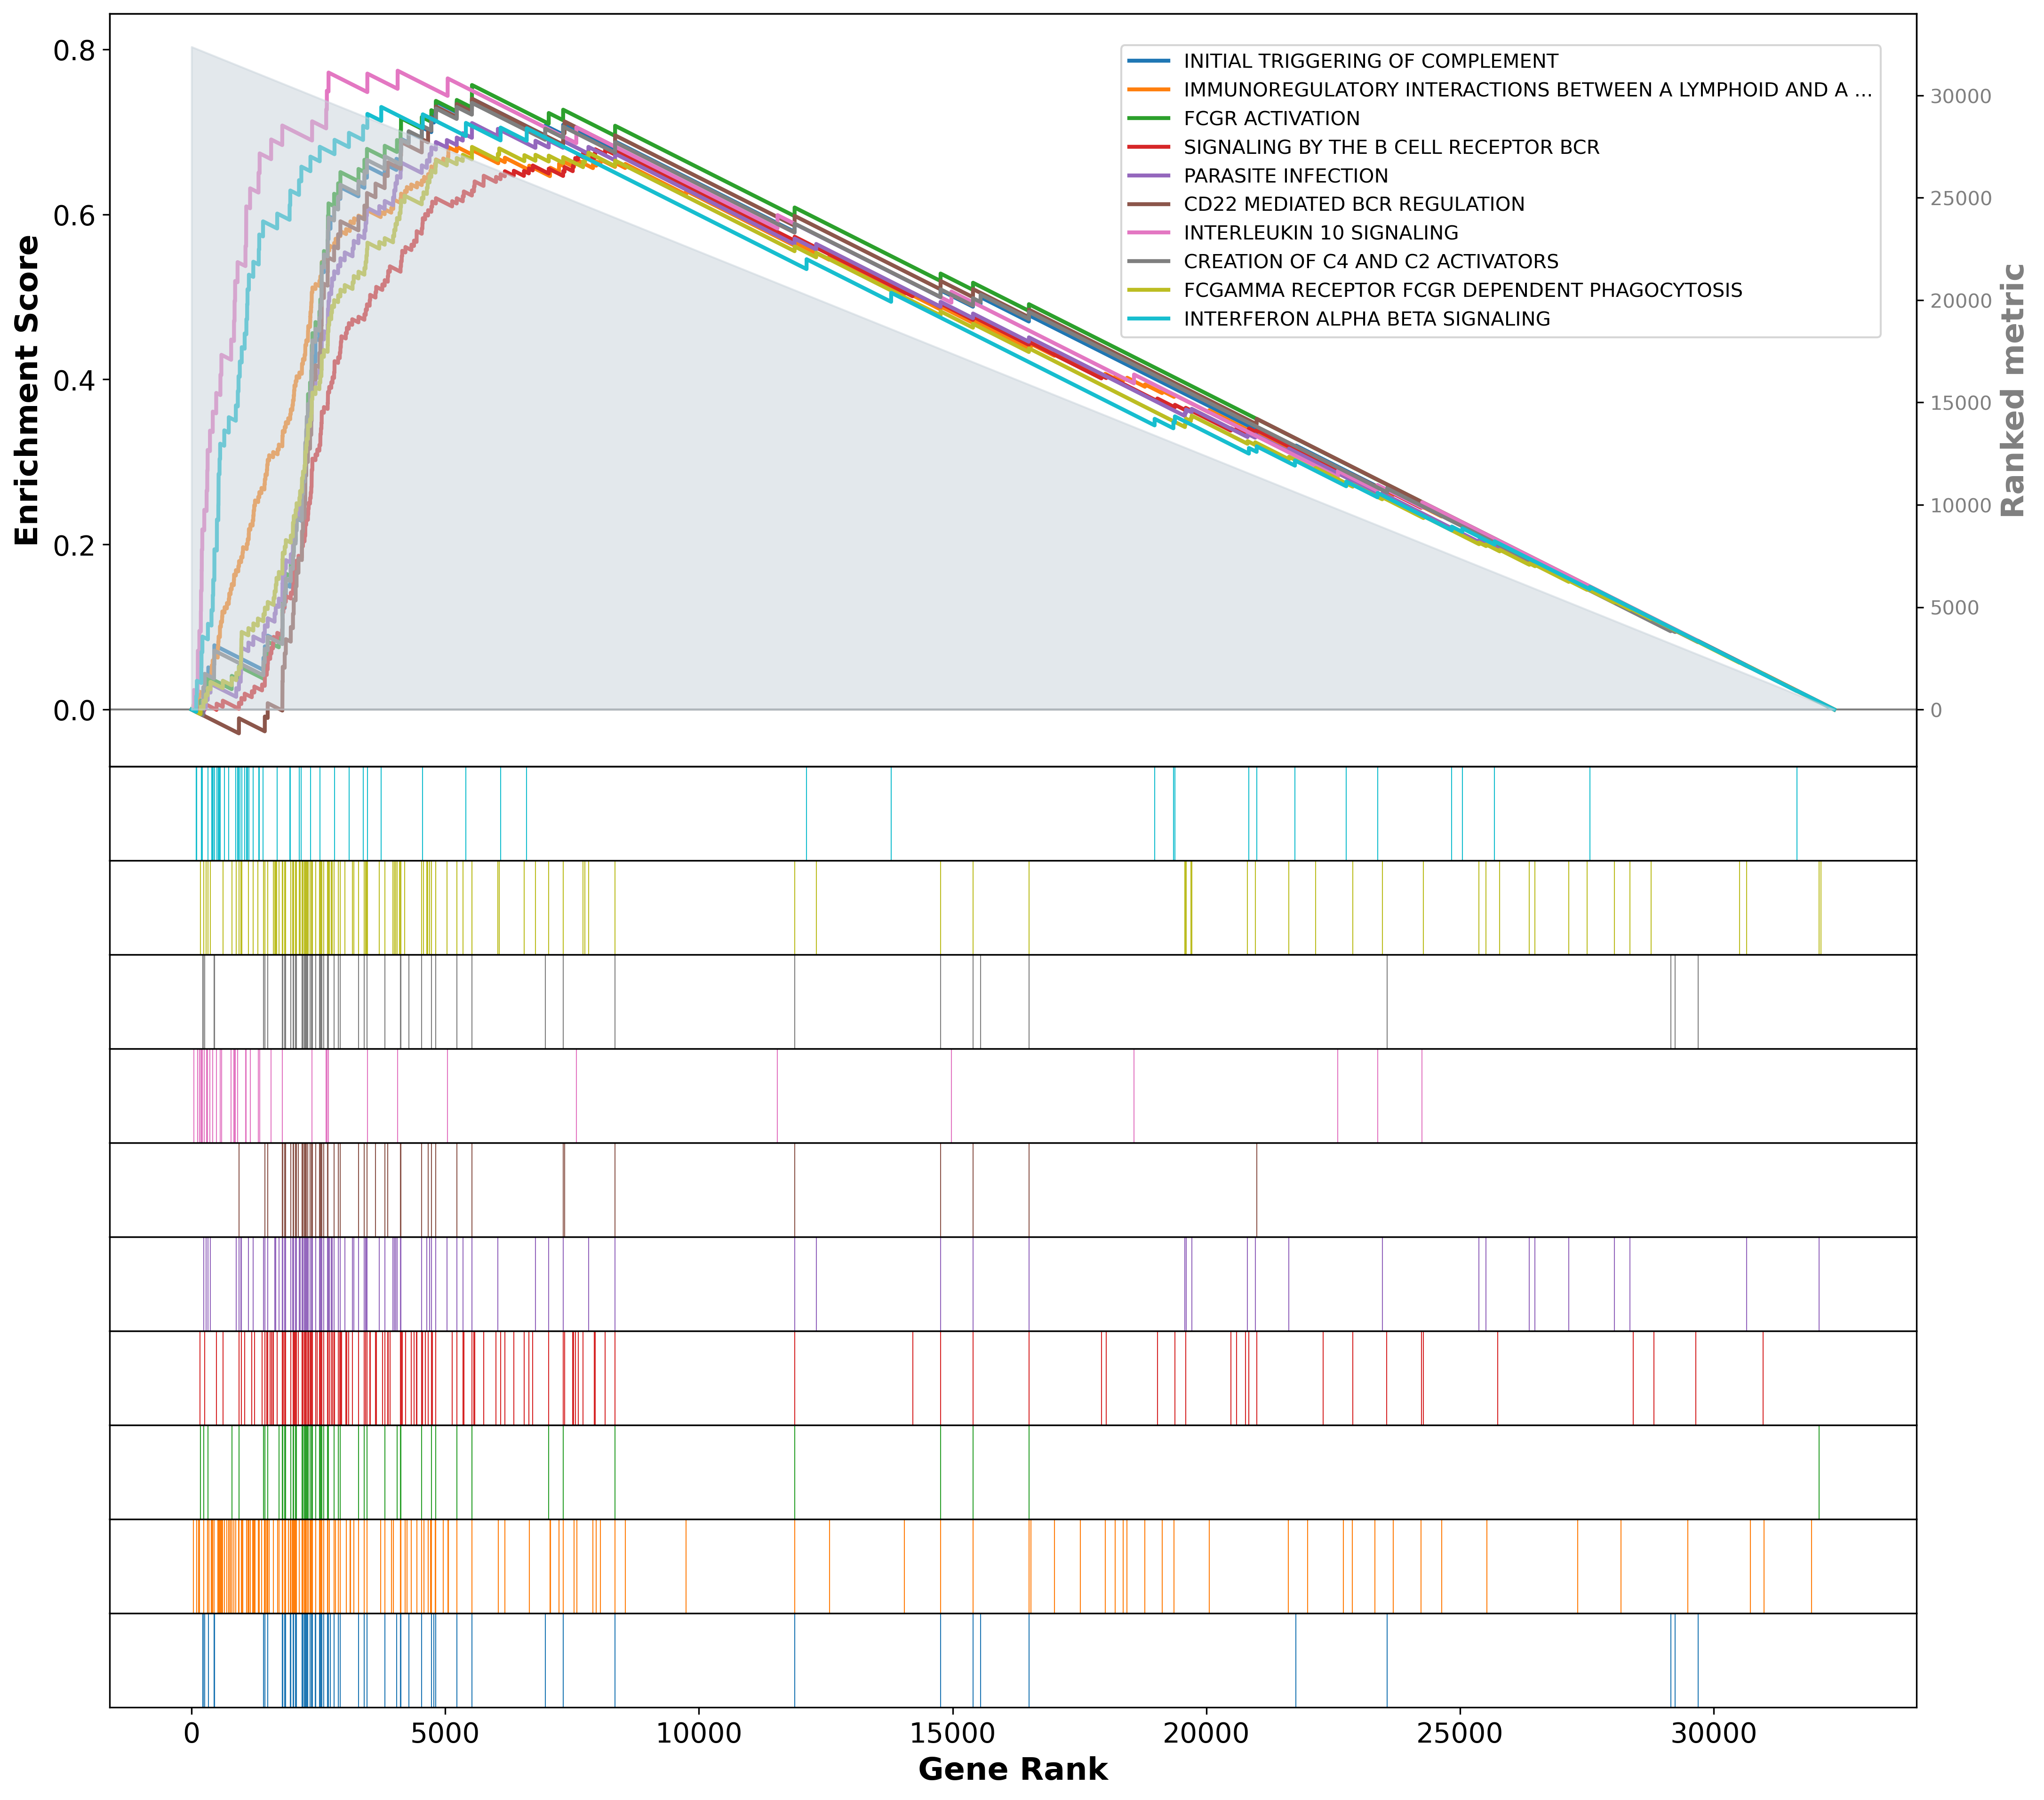
\includegraphics[width=\textwidth,keepaspectratio]{Sections/Network_I/Resources/selective_pruning/gsea/largeBasal_10_top_manTerms.png}
    \caption{GSEA output of the Basal group sfor the groups derived using Selective Edge pruning in  \cref{s:N_I:sel_tfs_subtypes}}
    \label{fig:ap:gsea_largeBasal}
\end{figure}

\begin{figure}[!htb]
    \centering
    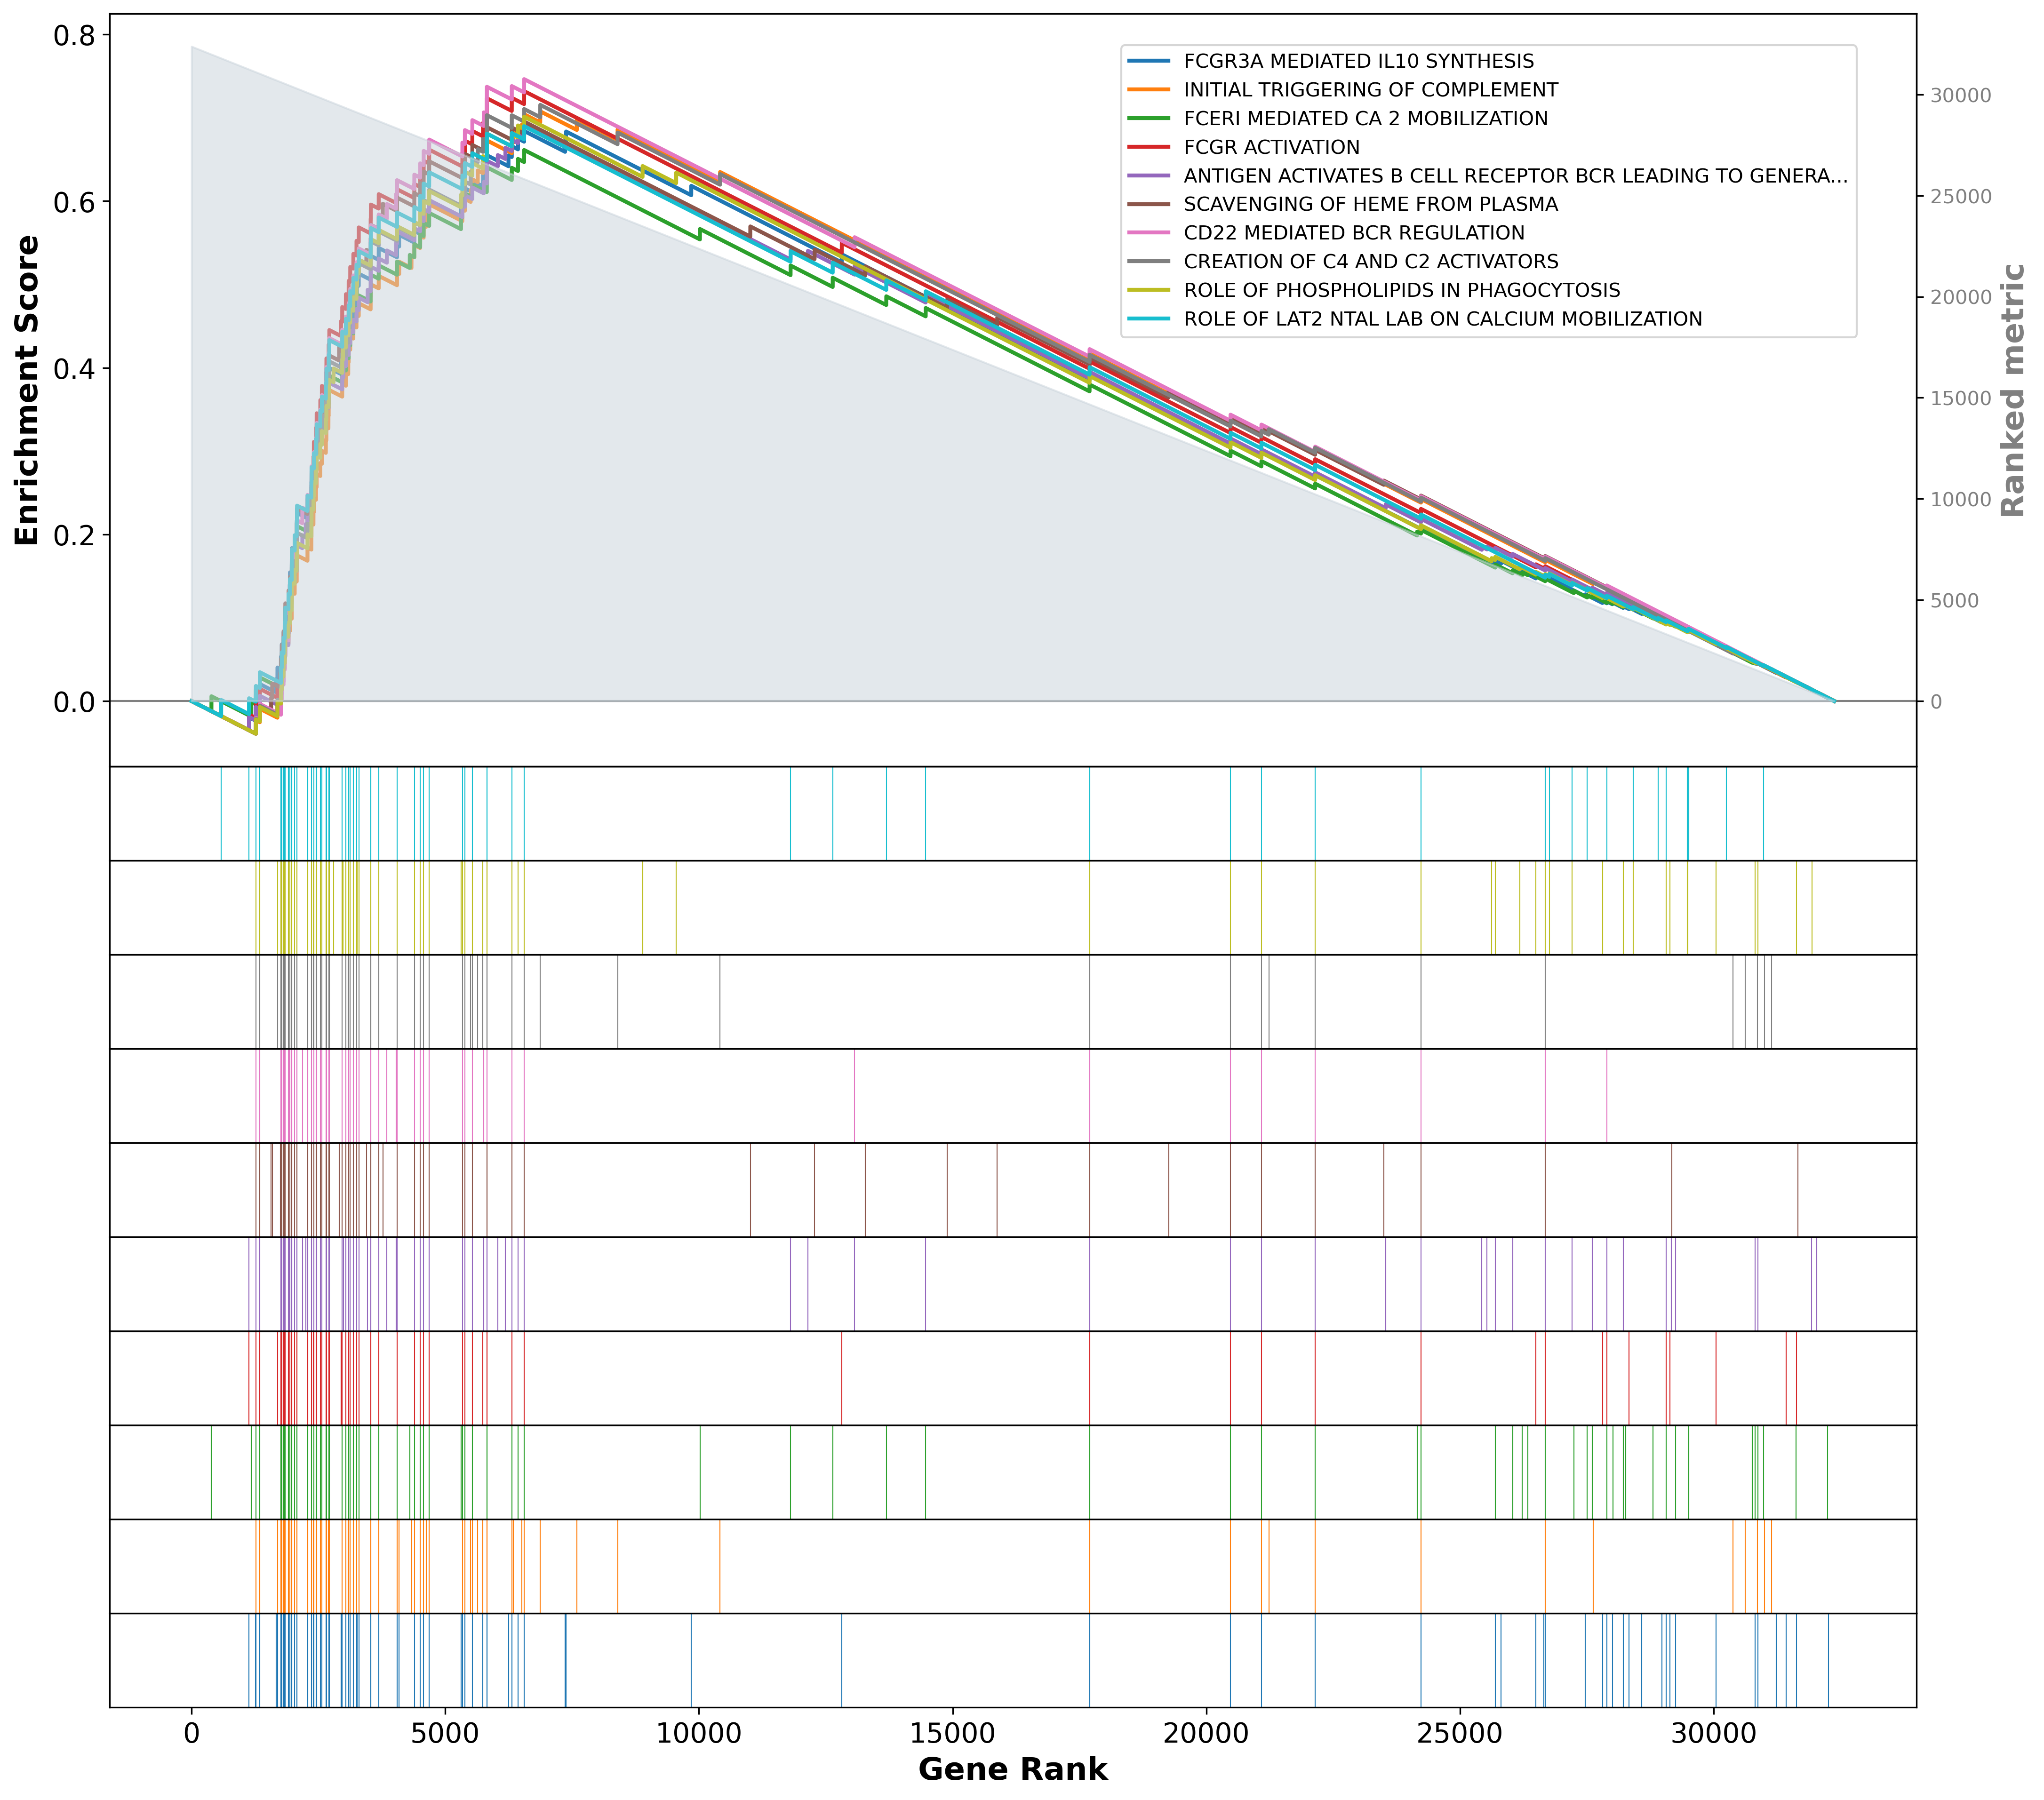
\includegraphics[width=\textwidth,keepaspectratio]{Sections/Network_I/Resources/selective_pruning/gsea/lumInf_10_top_manTerms.png}
    \caption{GSEA output of the Luminal Infiltrated group for the groups derived using Selective Edge pruning in  \cref{s:N_I:sel_tfs_subtypes}}
    \label{fig:ap:gsea_lumInf}
\end{figure}

\begin{figure}[!htb]
    \centering
    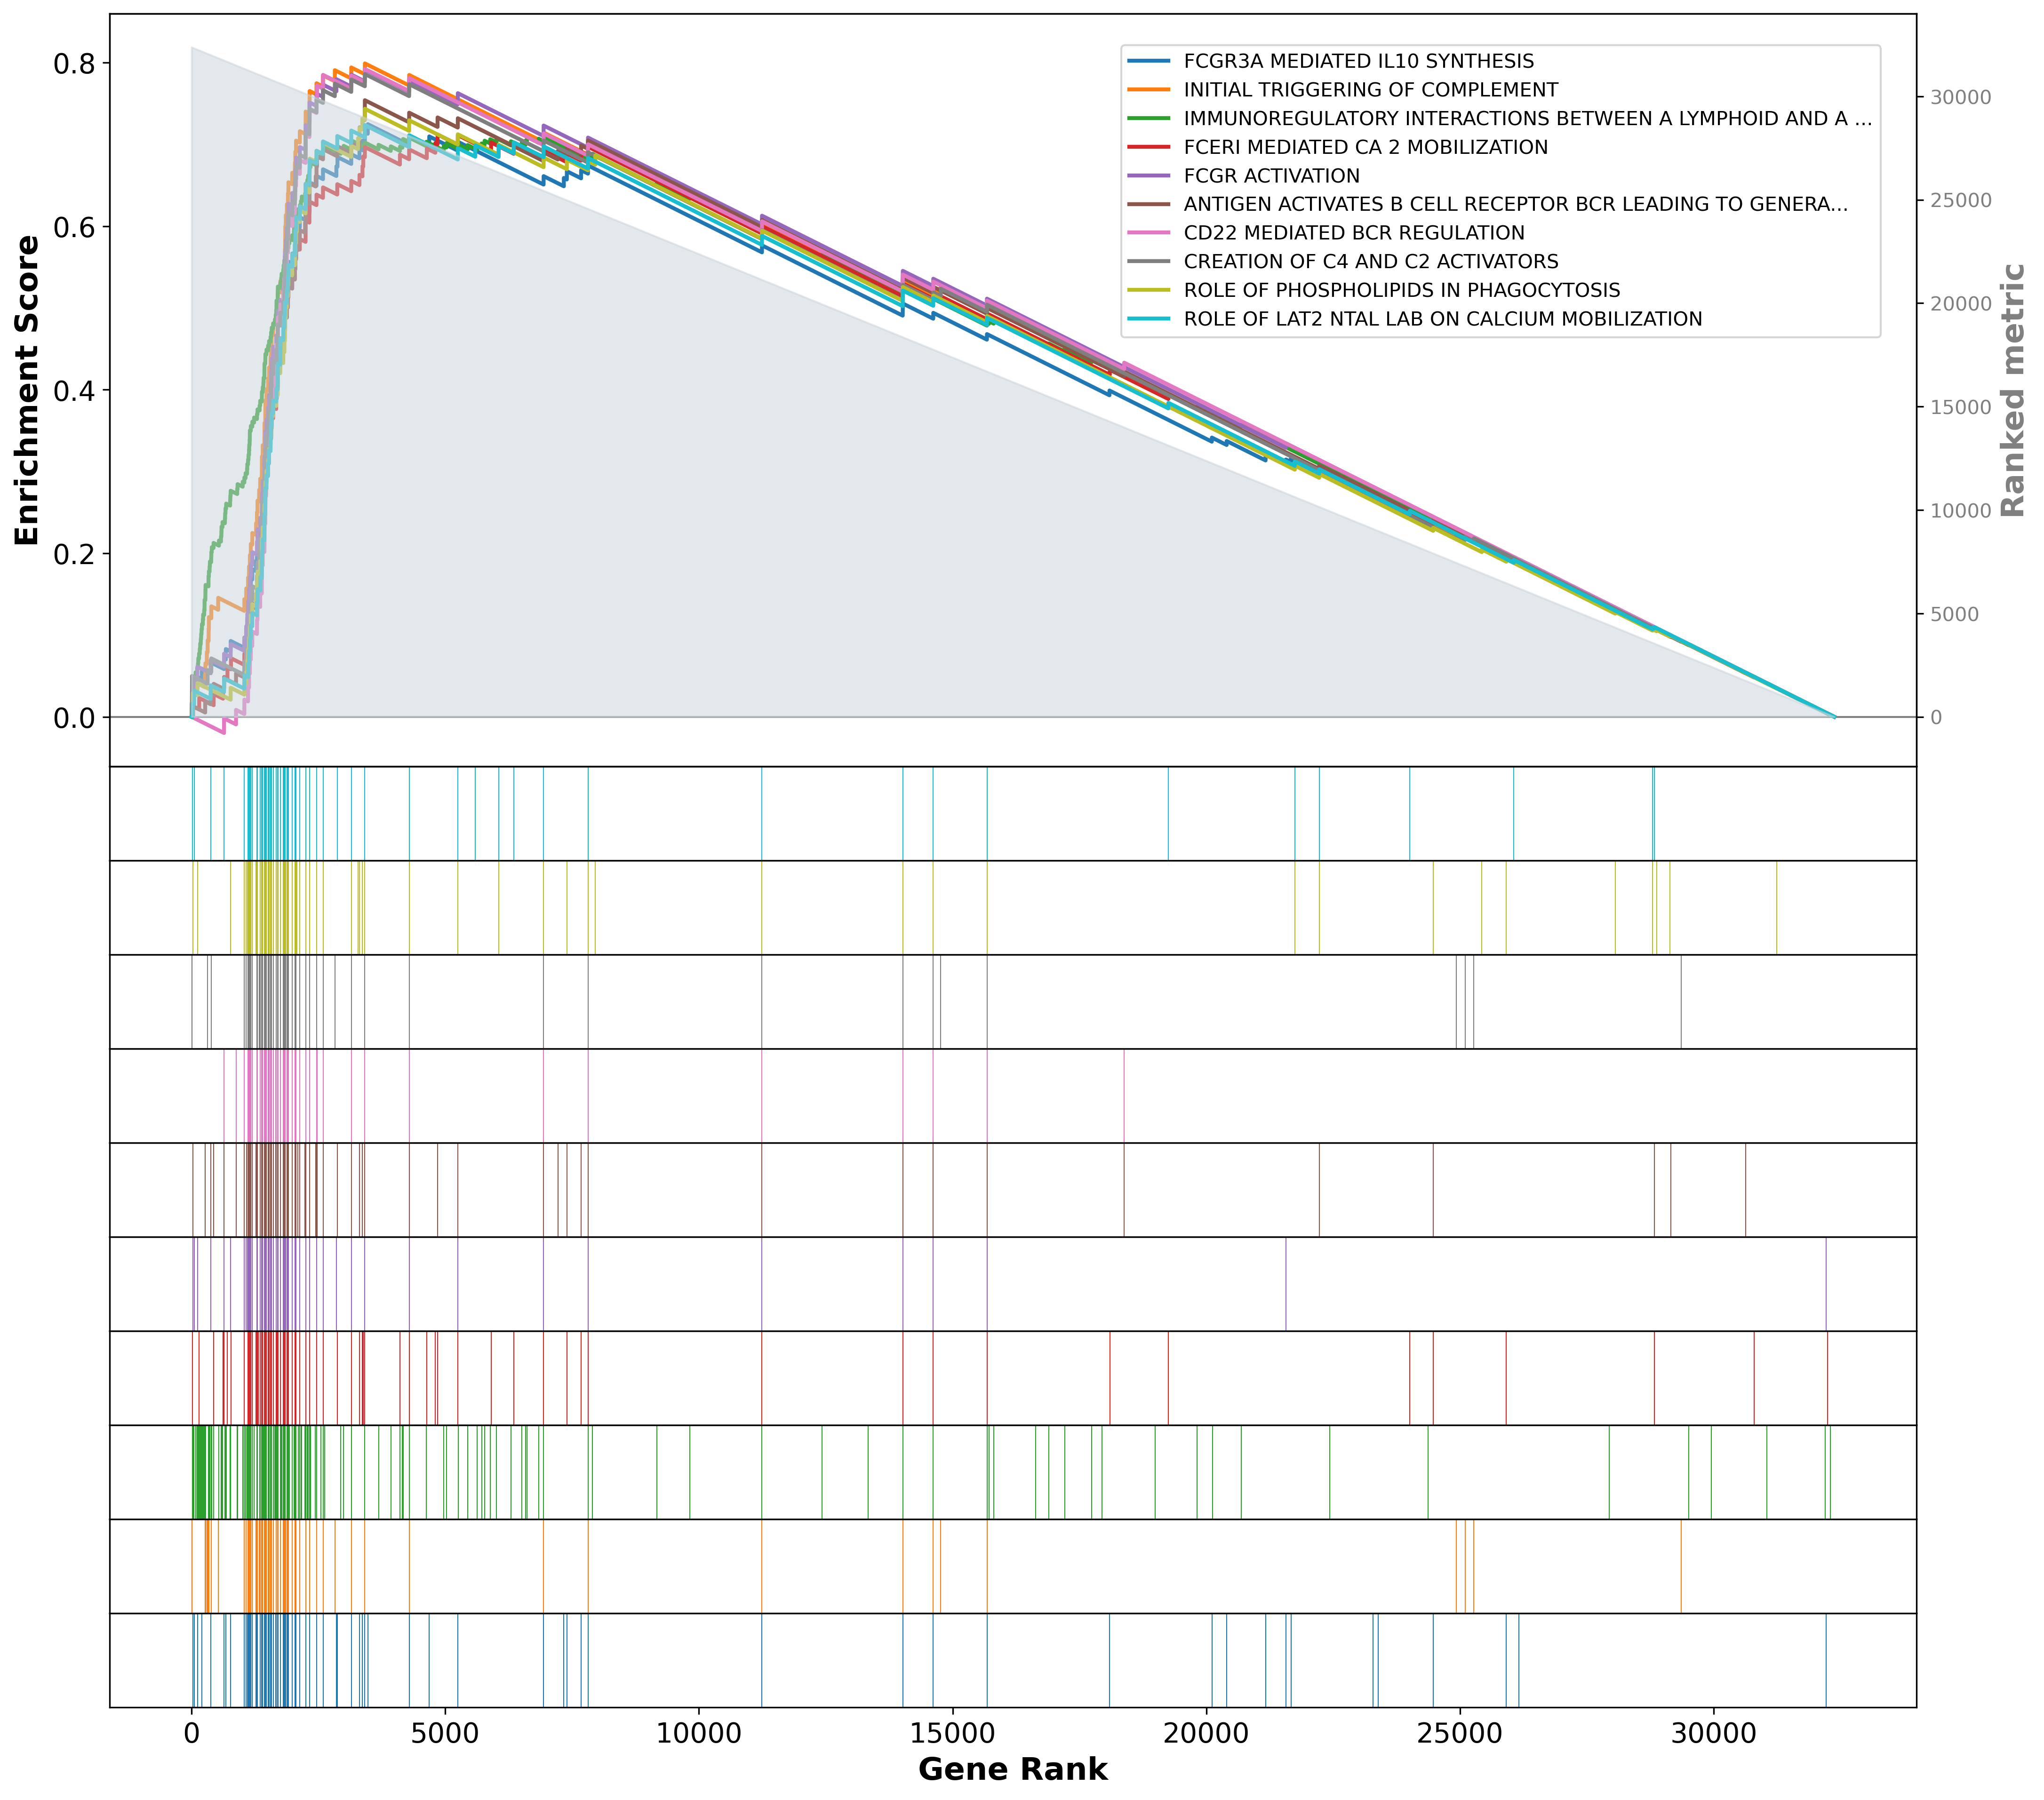
\includegraphics[width=\textwidth,keepaspectratio]{Sections/Network_I/Resources/selective_pruning/gsea/mesLike_10_top_manTerms.png}
    \caption{GSEA output of the Mes-like group for the groups derived using Selective Edge pruning in  \cref{s:N_I:sel_tfs_subtypes}}
    \label{fig:ap:gsea_mesLike}
\end{figure}

\begin{figure}[!htb]
    \centering
    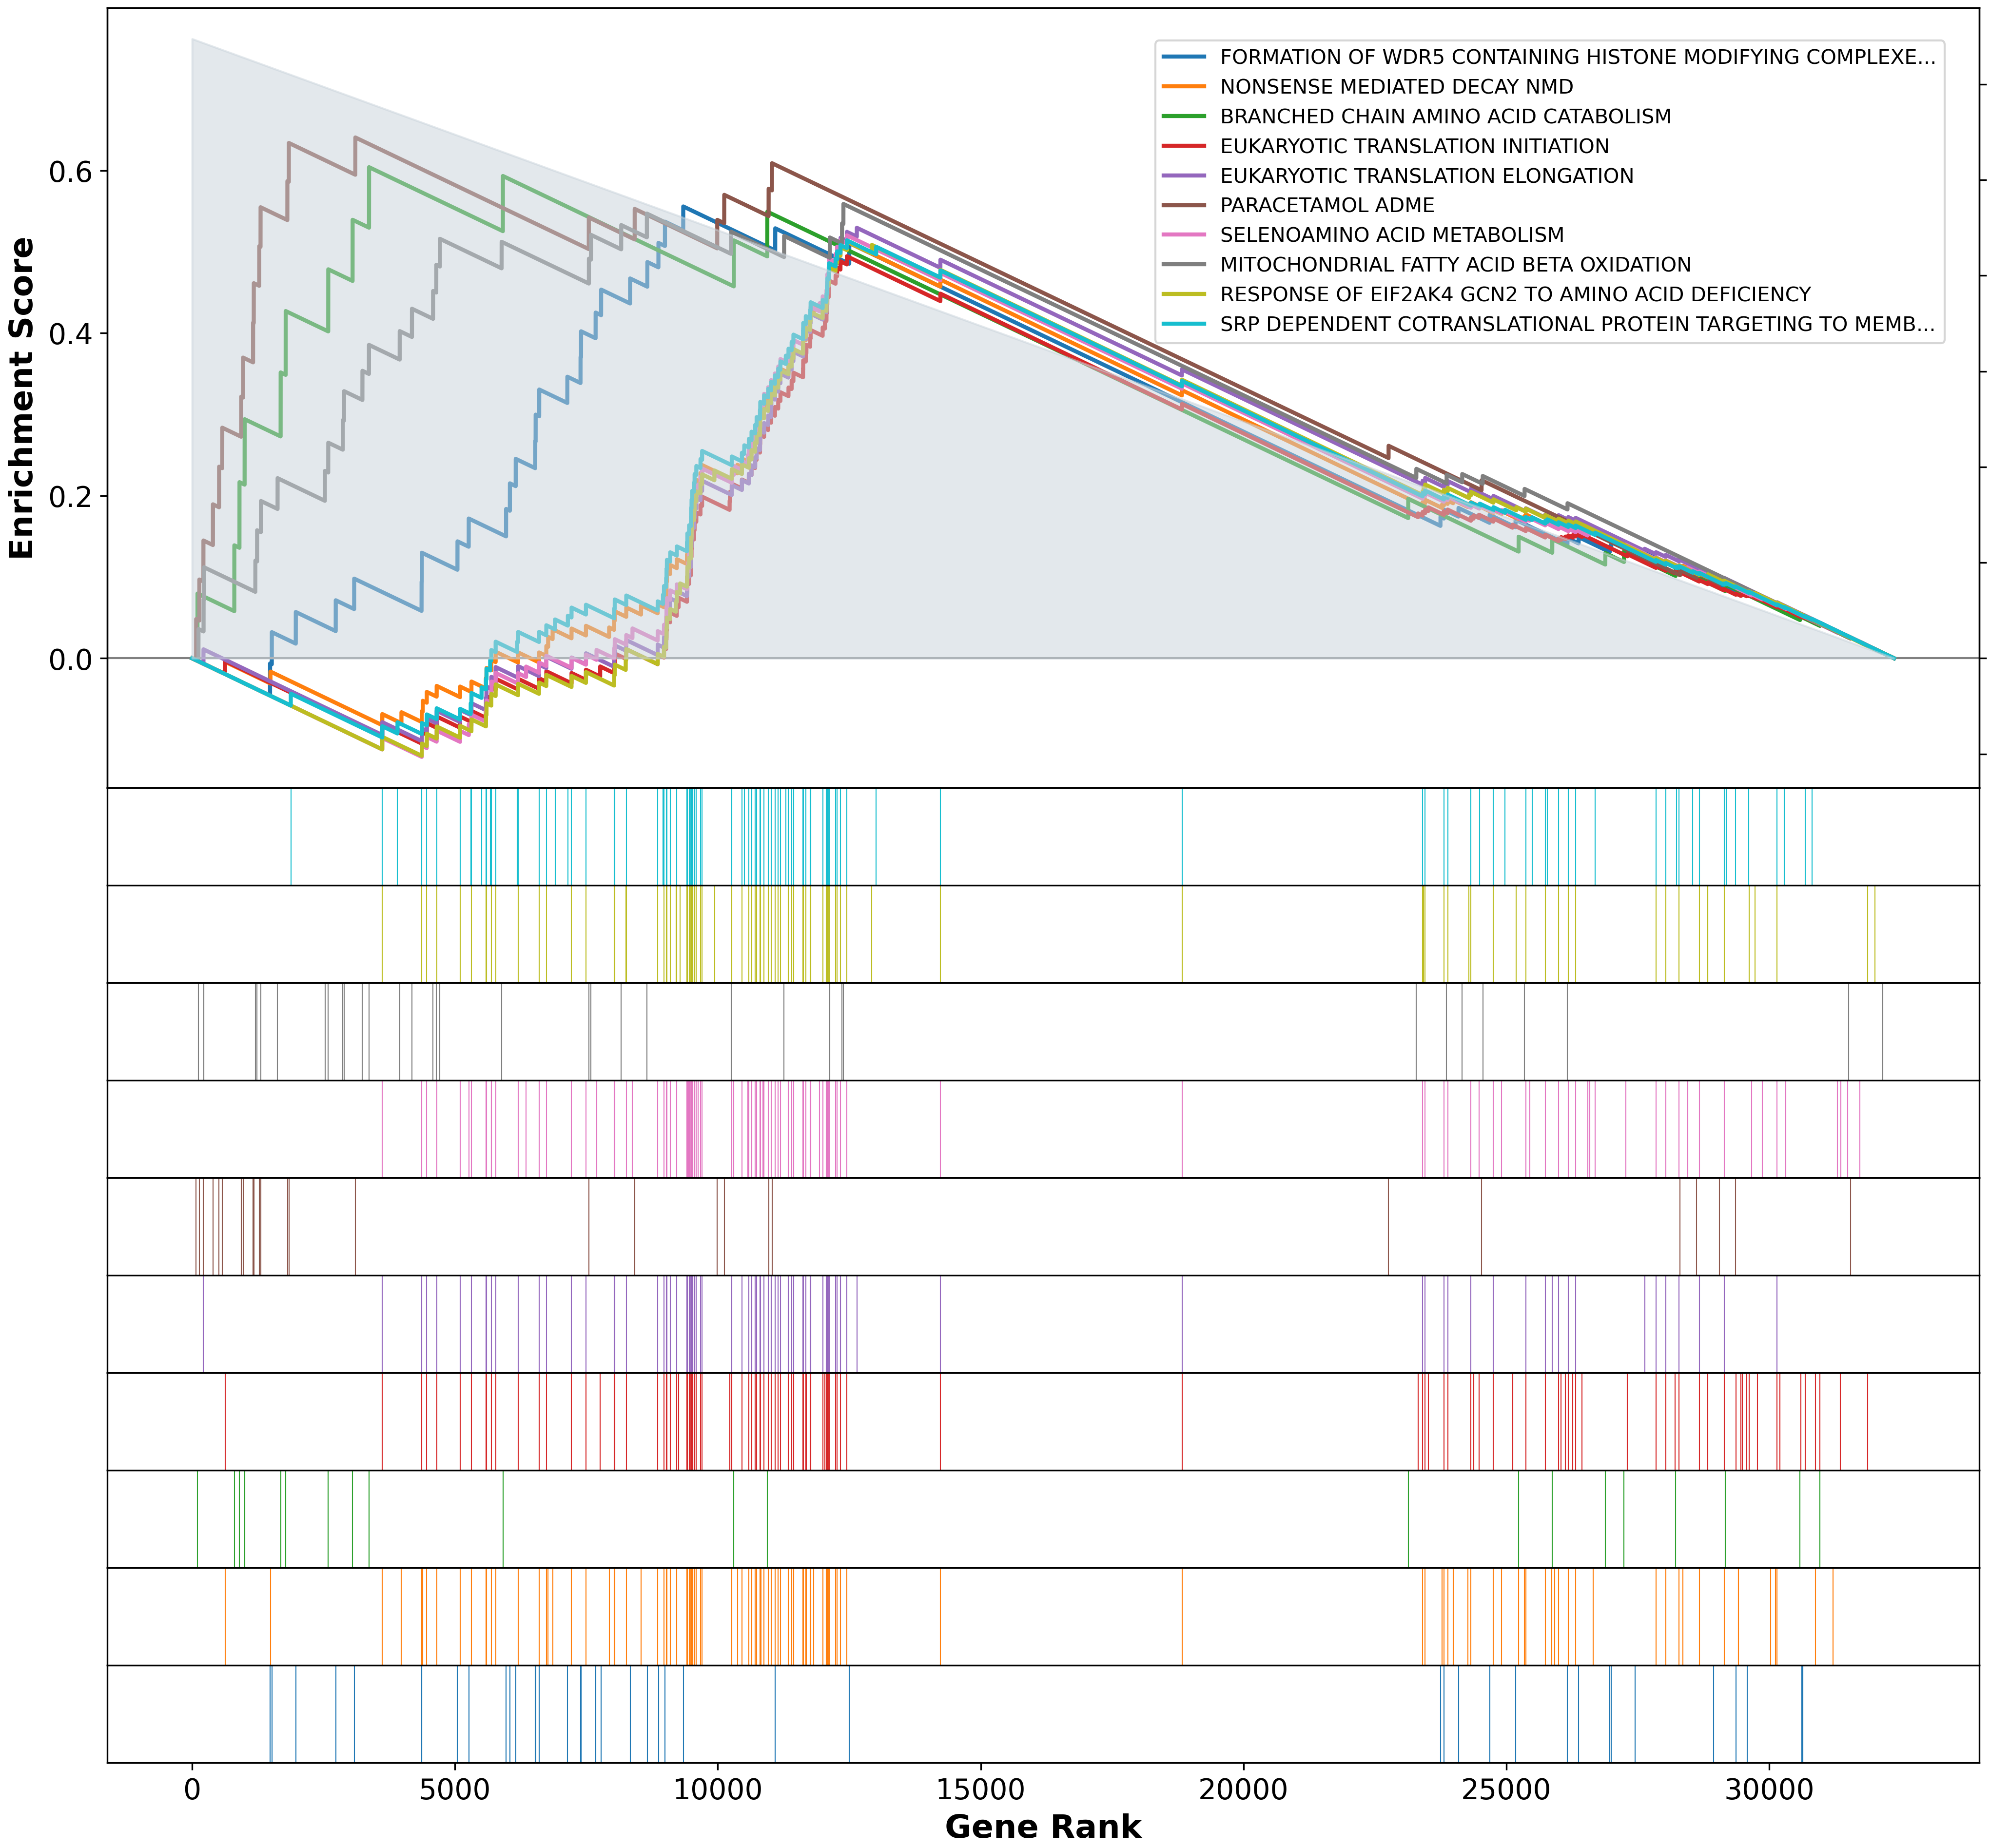
\includegraphics[width=\textwidth,keepaspectratio]{Sections/Network_I/Resources/selective_pruning/gsea/largeLuminal_10_top_manTerms.png}
    \caption{GSEA output of the Luminal group for the groups derived using Selective Edge pruning in  \cref{s:N_I:sel_tfs_subtypes}}
    \label{fig:ap:gsea_largeLuminal}
\end{figure}

% \begin{figure}[!h]
%     \captionsetup[subfigure]{justification=centering}
%     \centering
%     \begin{subfigure}[!t]{0.4\textwidth}
%         \centering
%         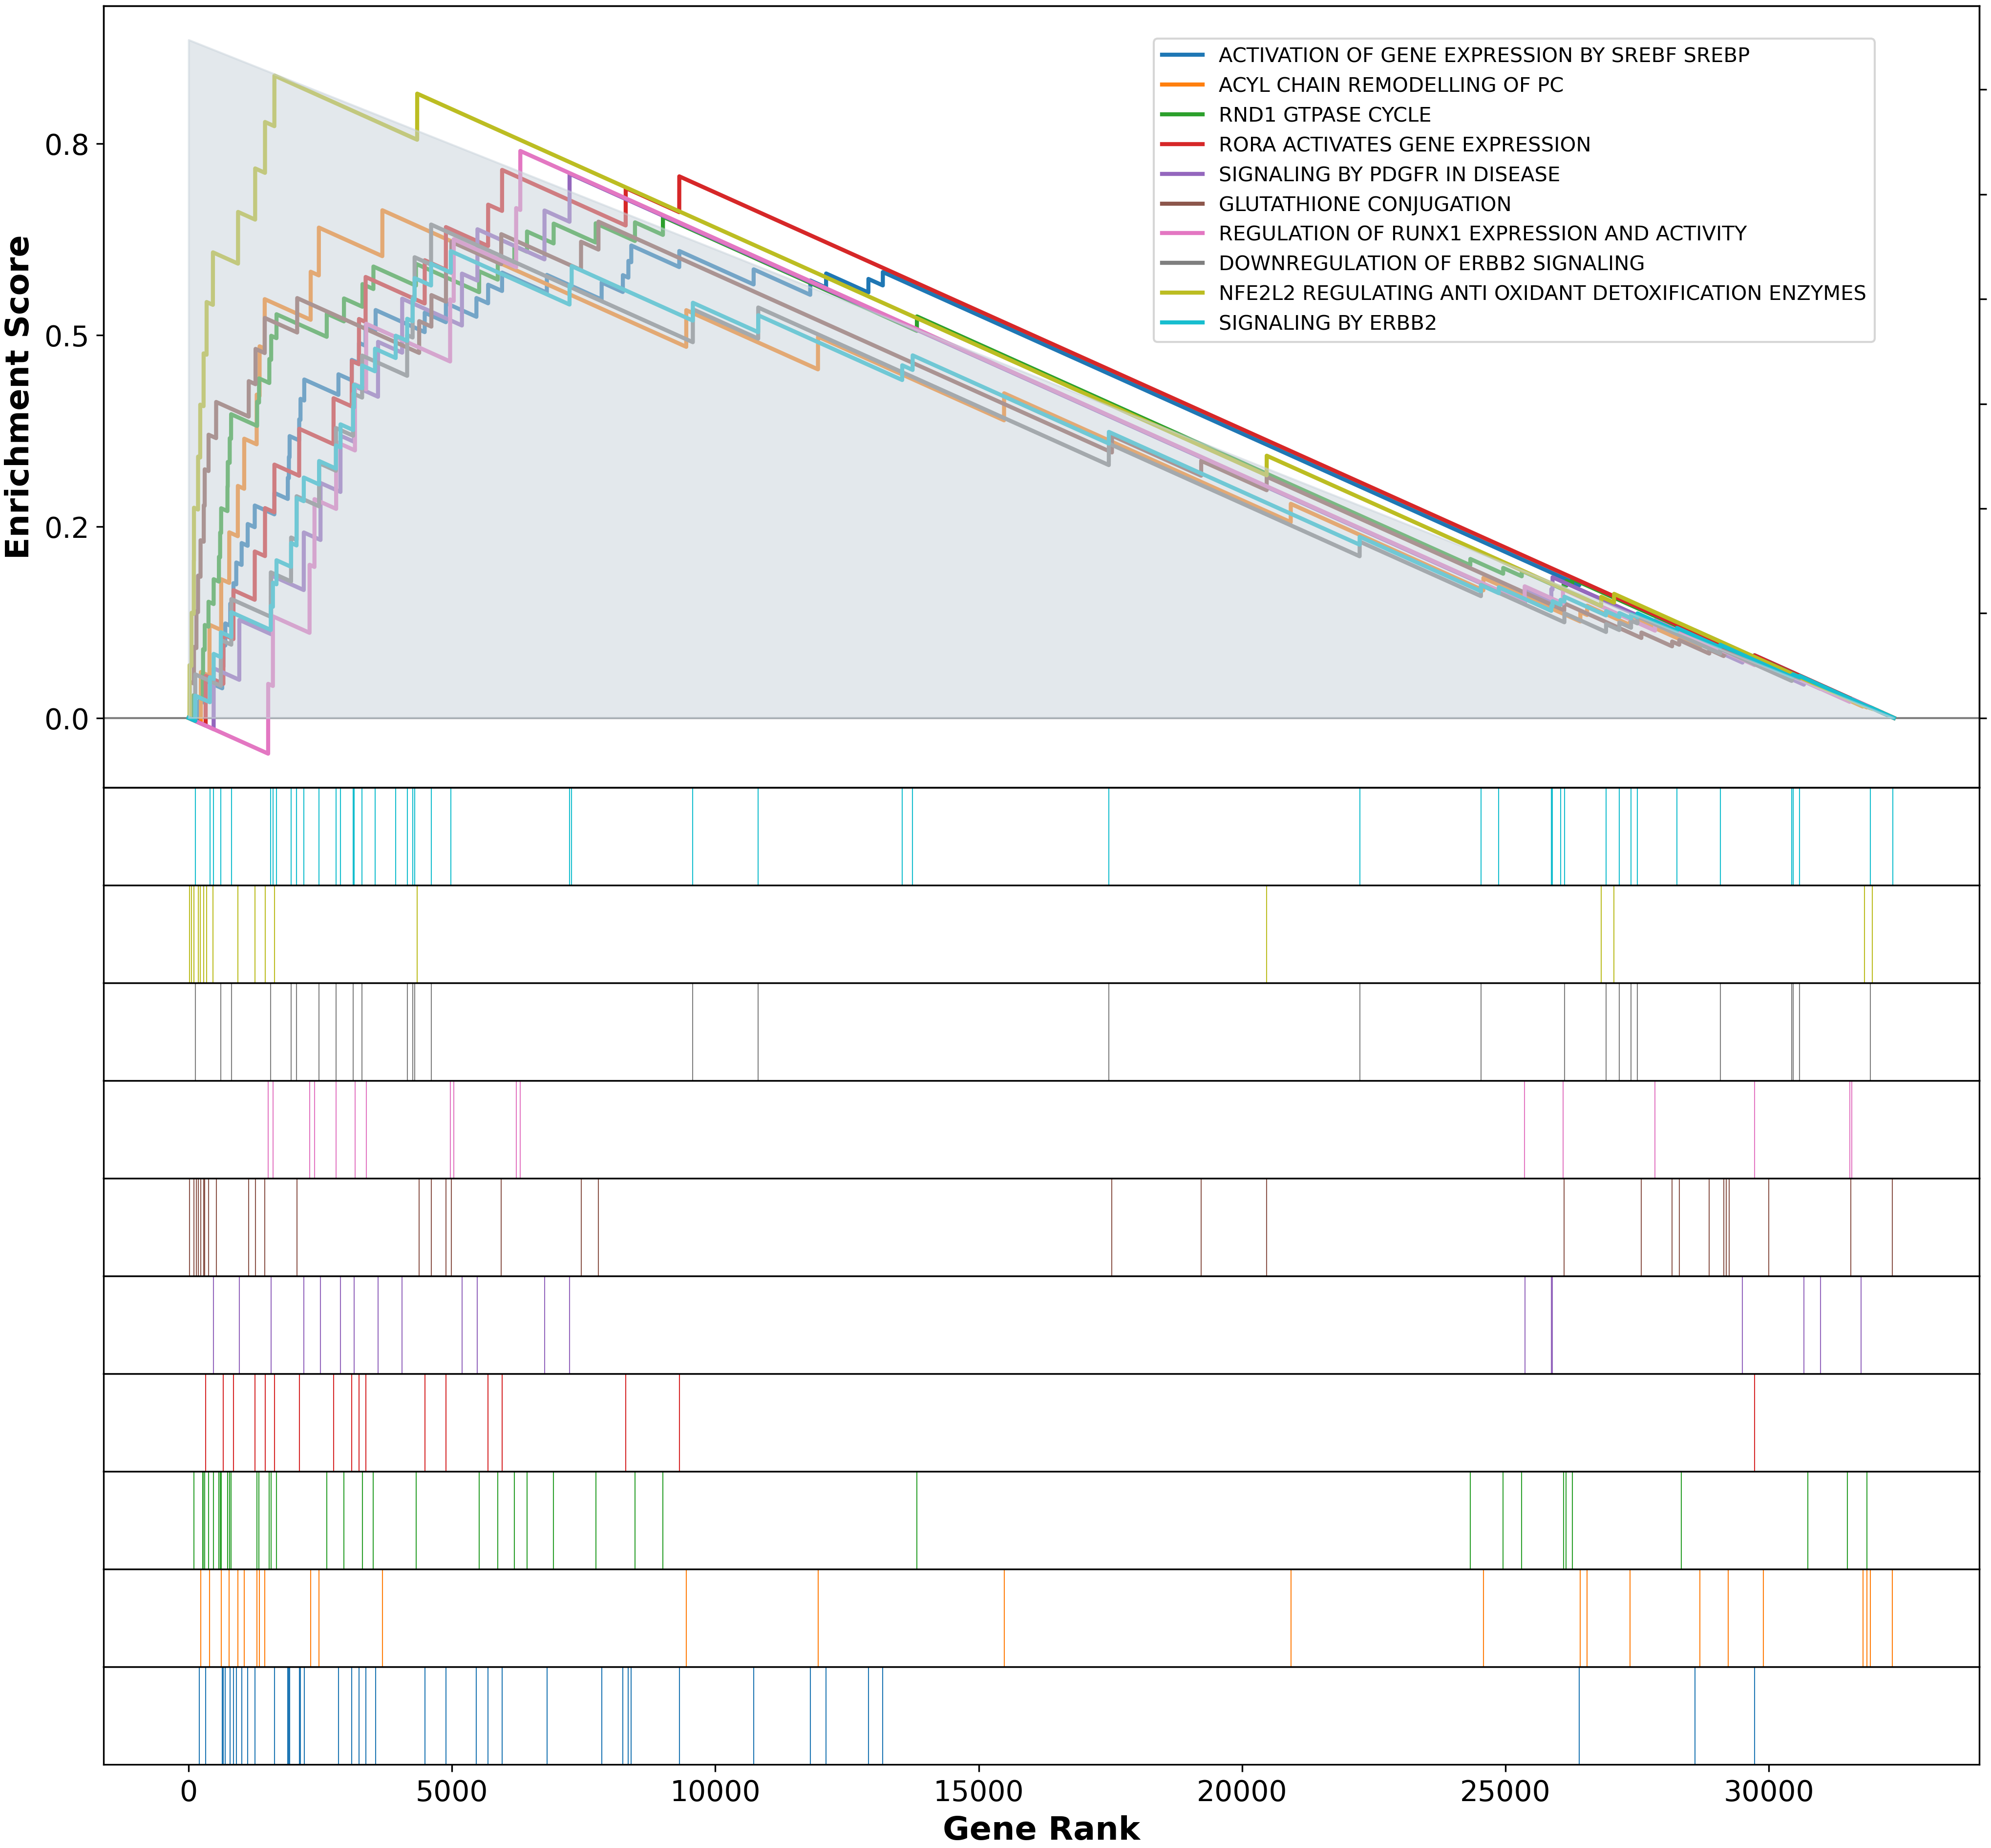
\includegraphics[width=\textwidth,keepaspectratio]{Sections/Network_I/Resources/selective_pruning/gsea/smallBasal_10_top_manTerms.png}
%         \caption{Small Basal}
%         \label{fig:ap:gsea_smallBasal}
%     \end{subfigure}
%     \begin{subfigure}[!t]{0.4\textwidth}
%         \centering
%         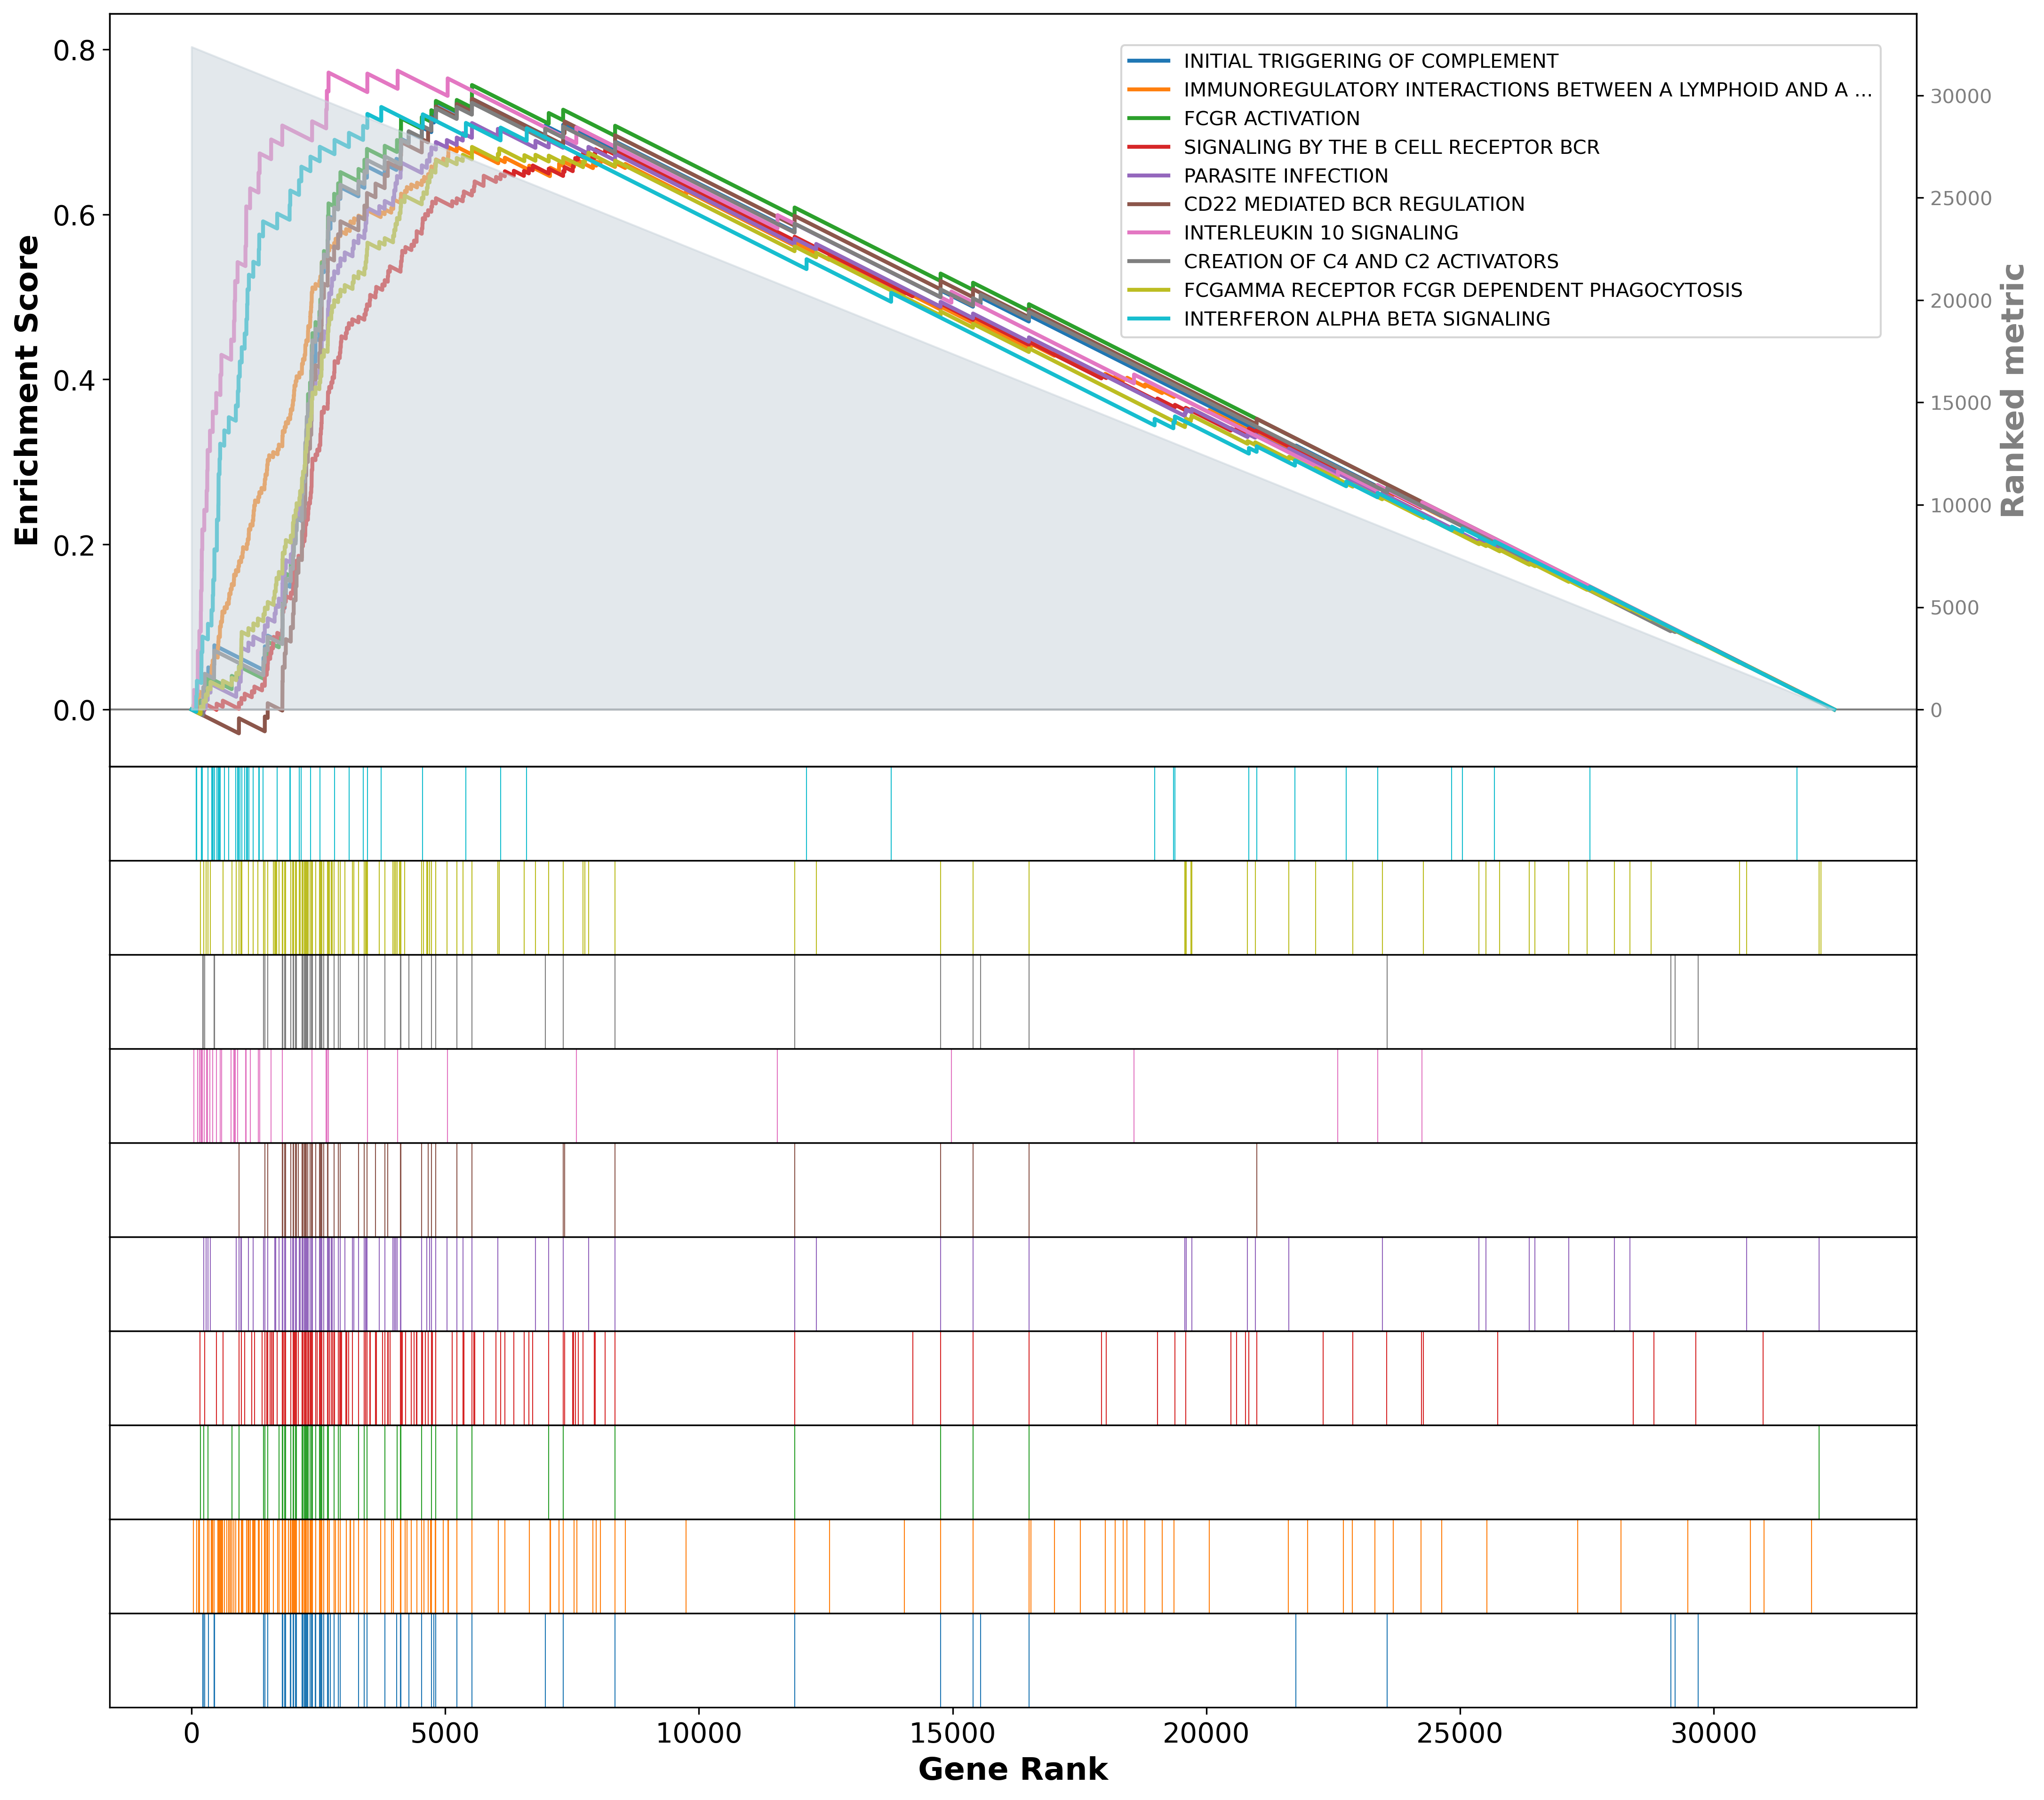
\includegraphics[width=\textwidth,keepaspectratio]{Sections/Network_I/Resources/selective_pruning/gsea/largeBasal_10_top_manTerms.png}
%         \caption{Large Basal}
%         \label{fig:ap:gsea_largeBasal}
%     \end{subfigure} 
%     \begin{subfigure}[!t]{0.4\textwidth}
%         \centering
%         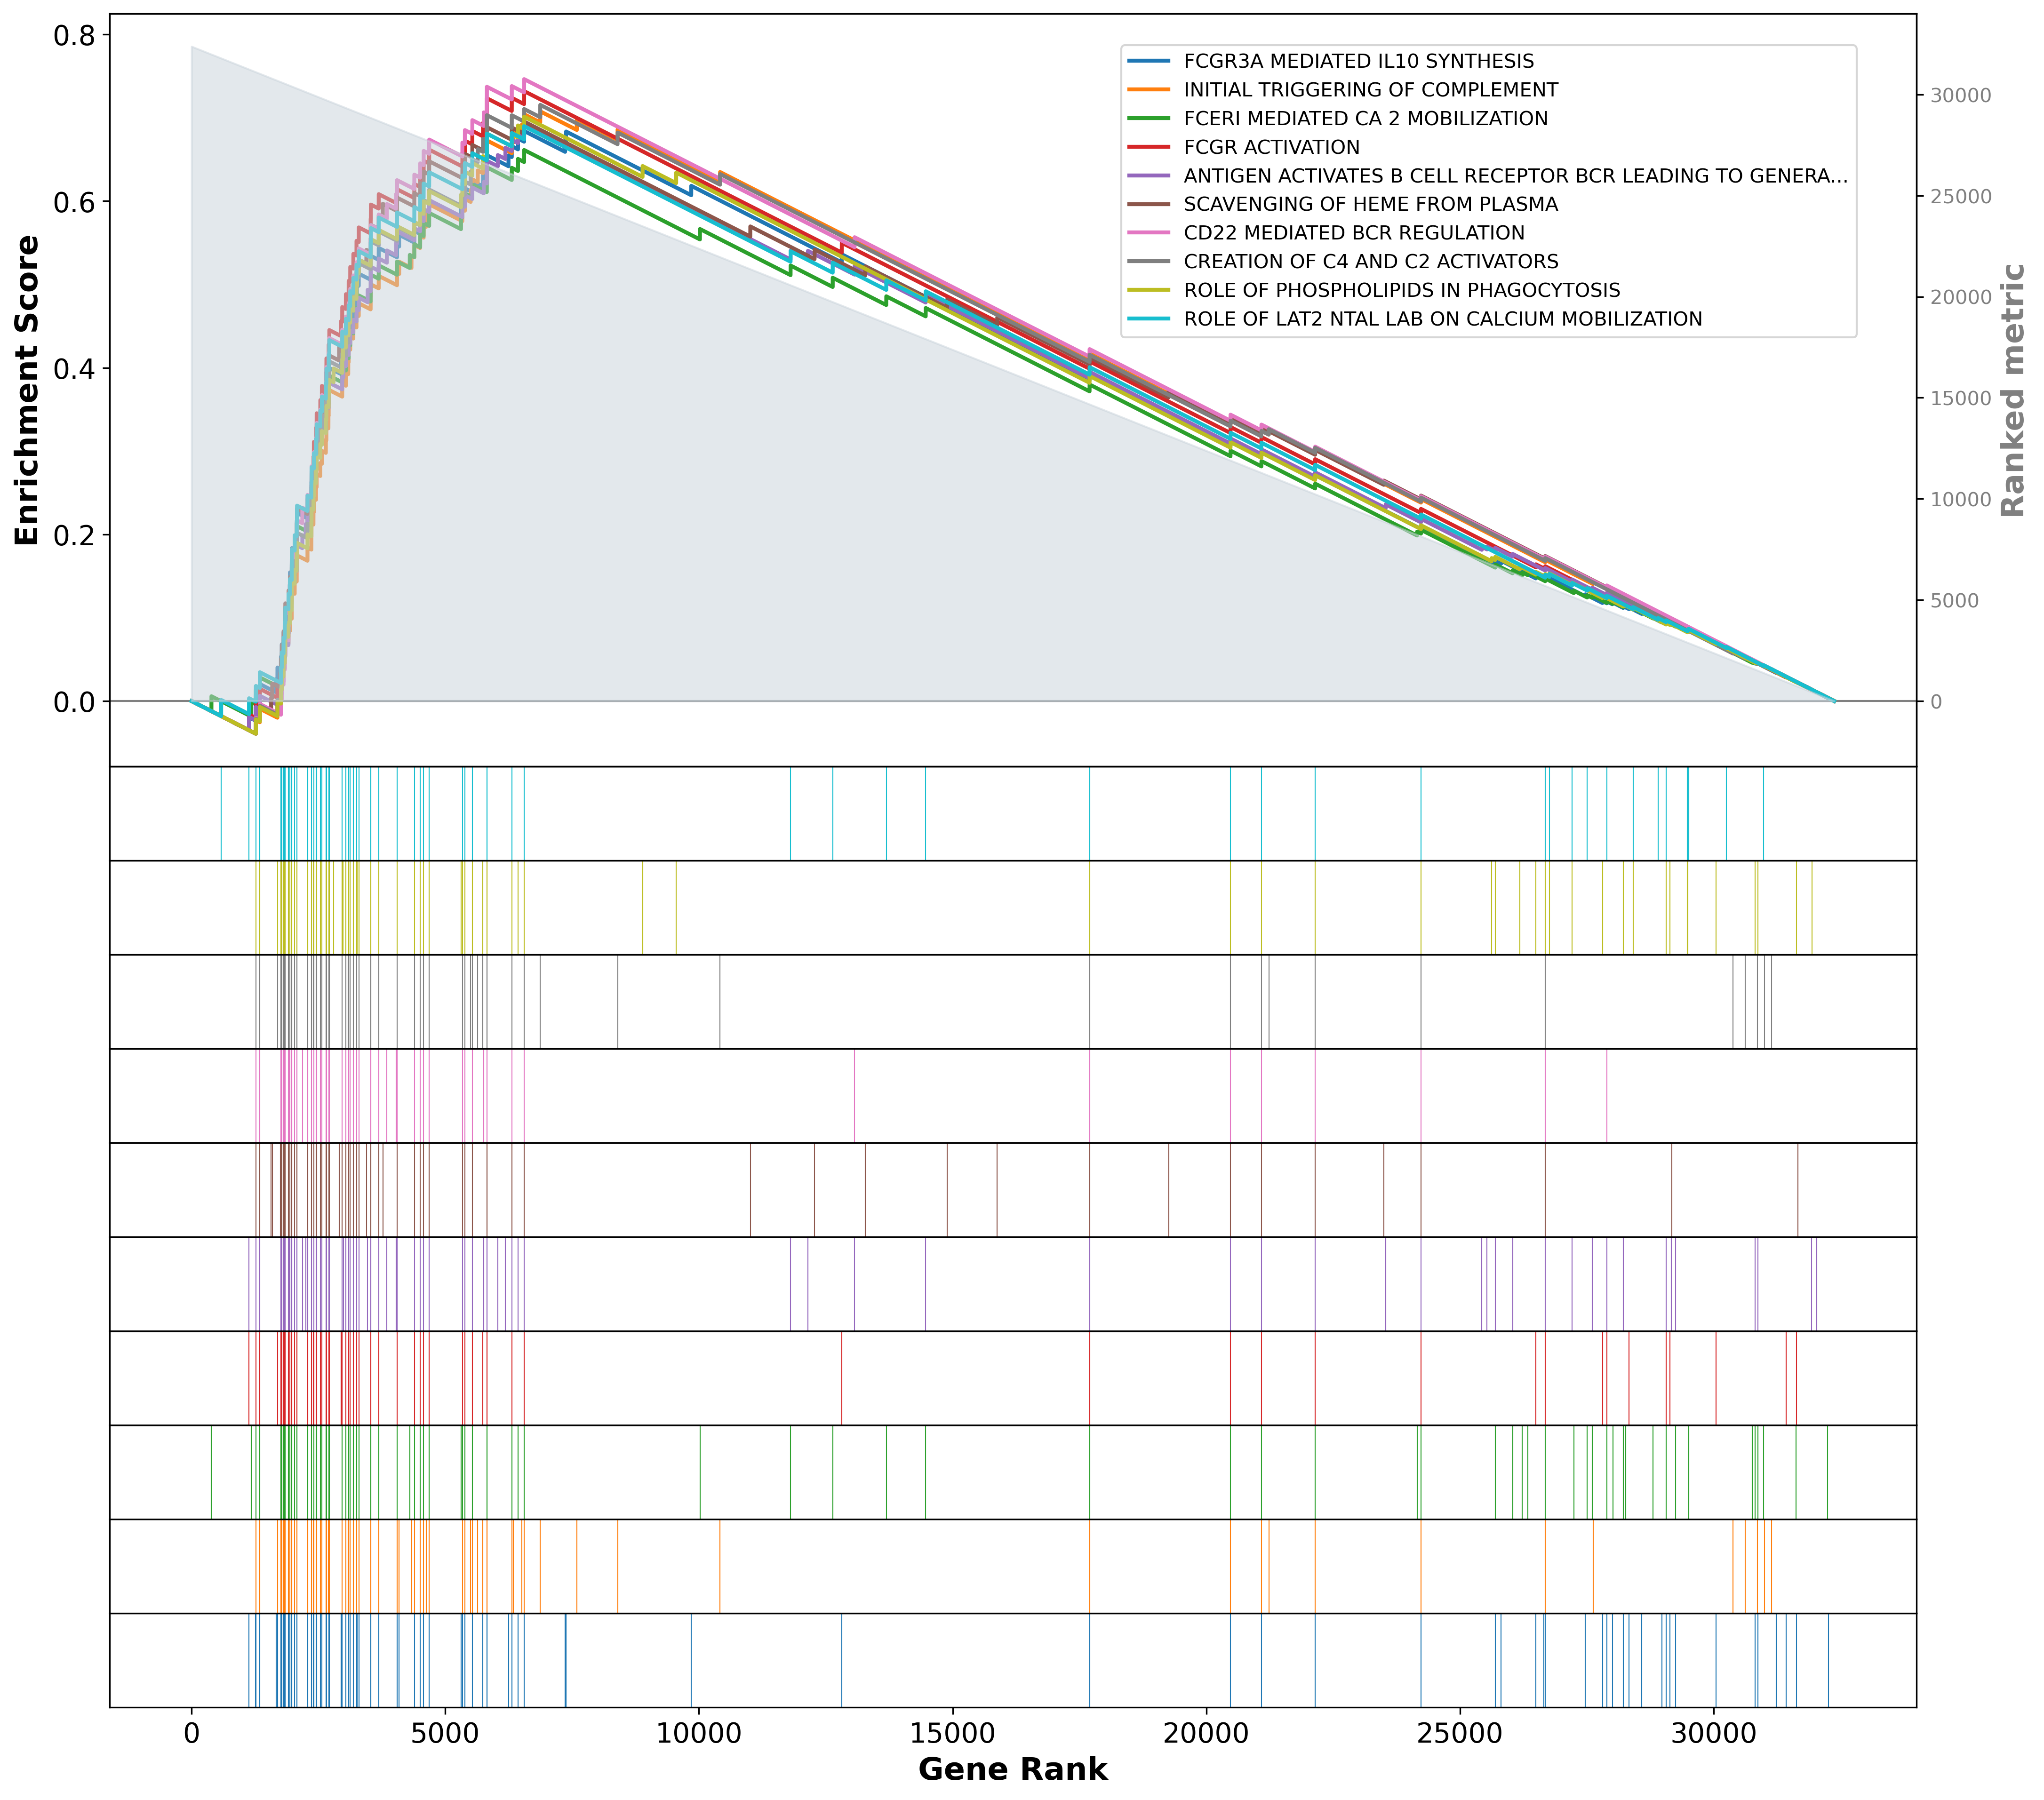
\includegraphics[width=\textwidth,keepaspectratio]{Sections/Network_I/Resources/selective_pruning/gsea/lumInf_10_top_manTerms.png}
%         \caption{Luminal Infiltrated}
%         \label{fig:ap:gsea_lumInf}
%     \end{subfigure}
%     \begin{subfigure}[!t]{0.4\textwidth}
%         \centering
%         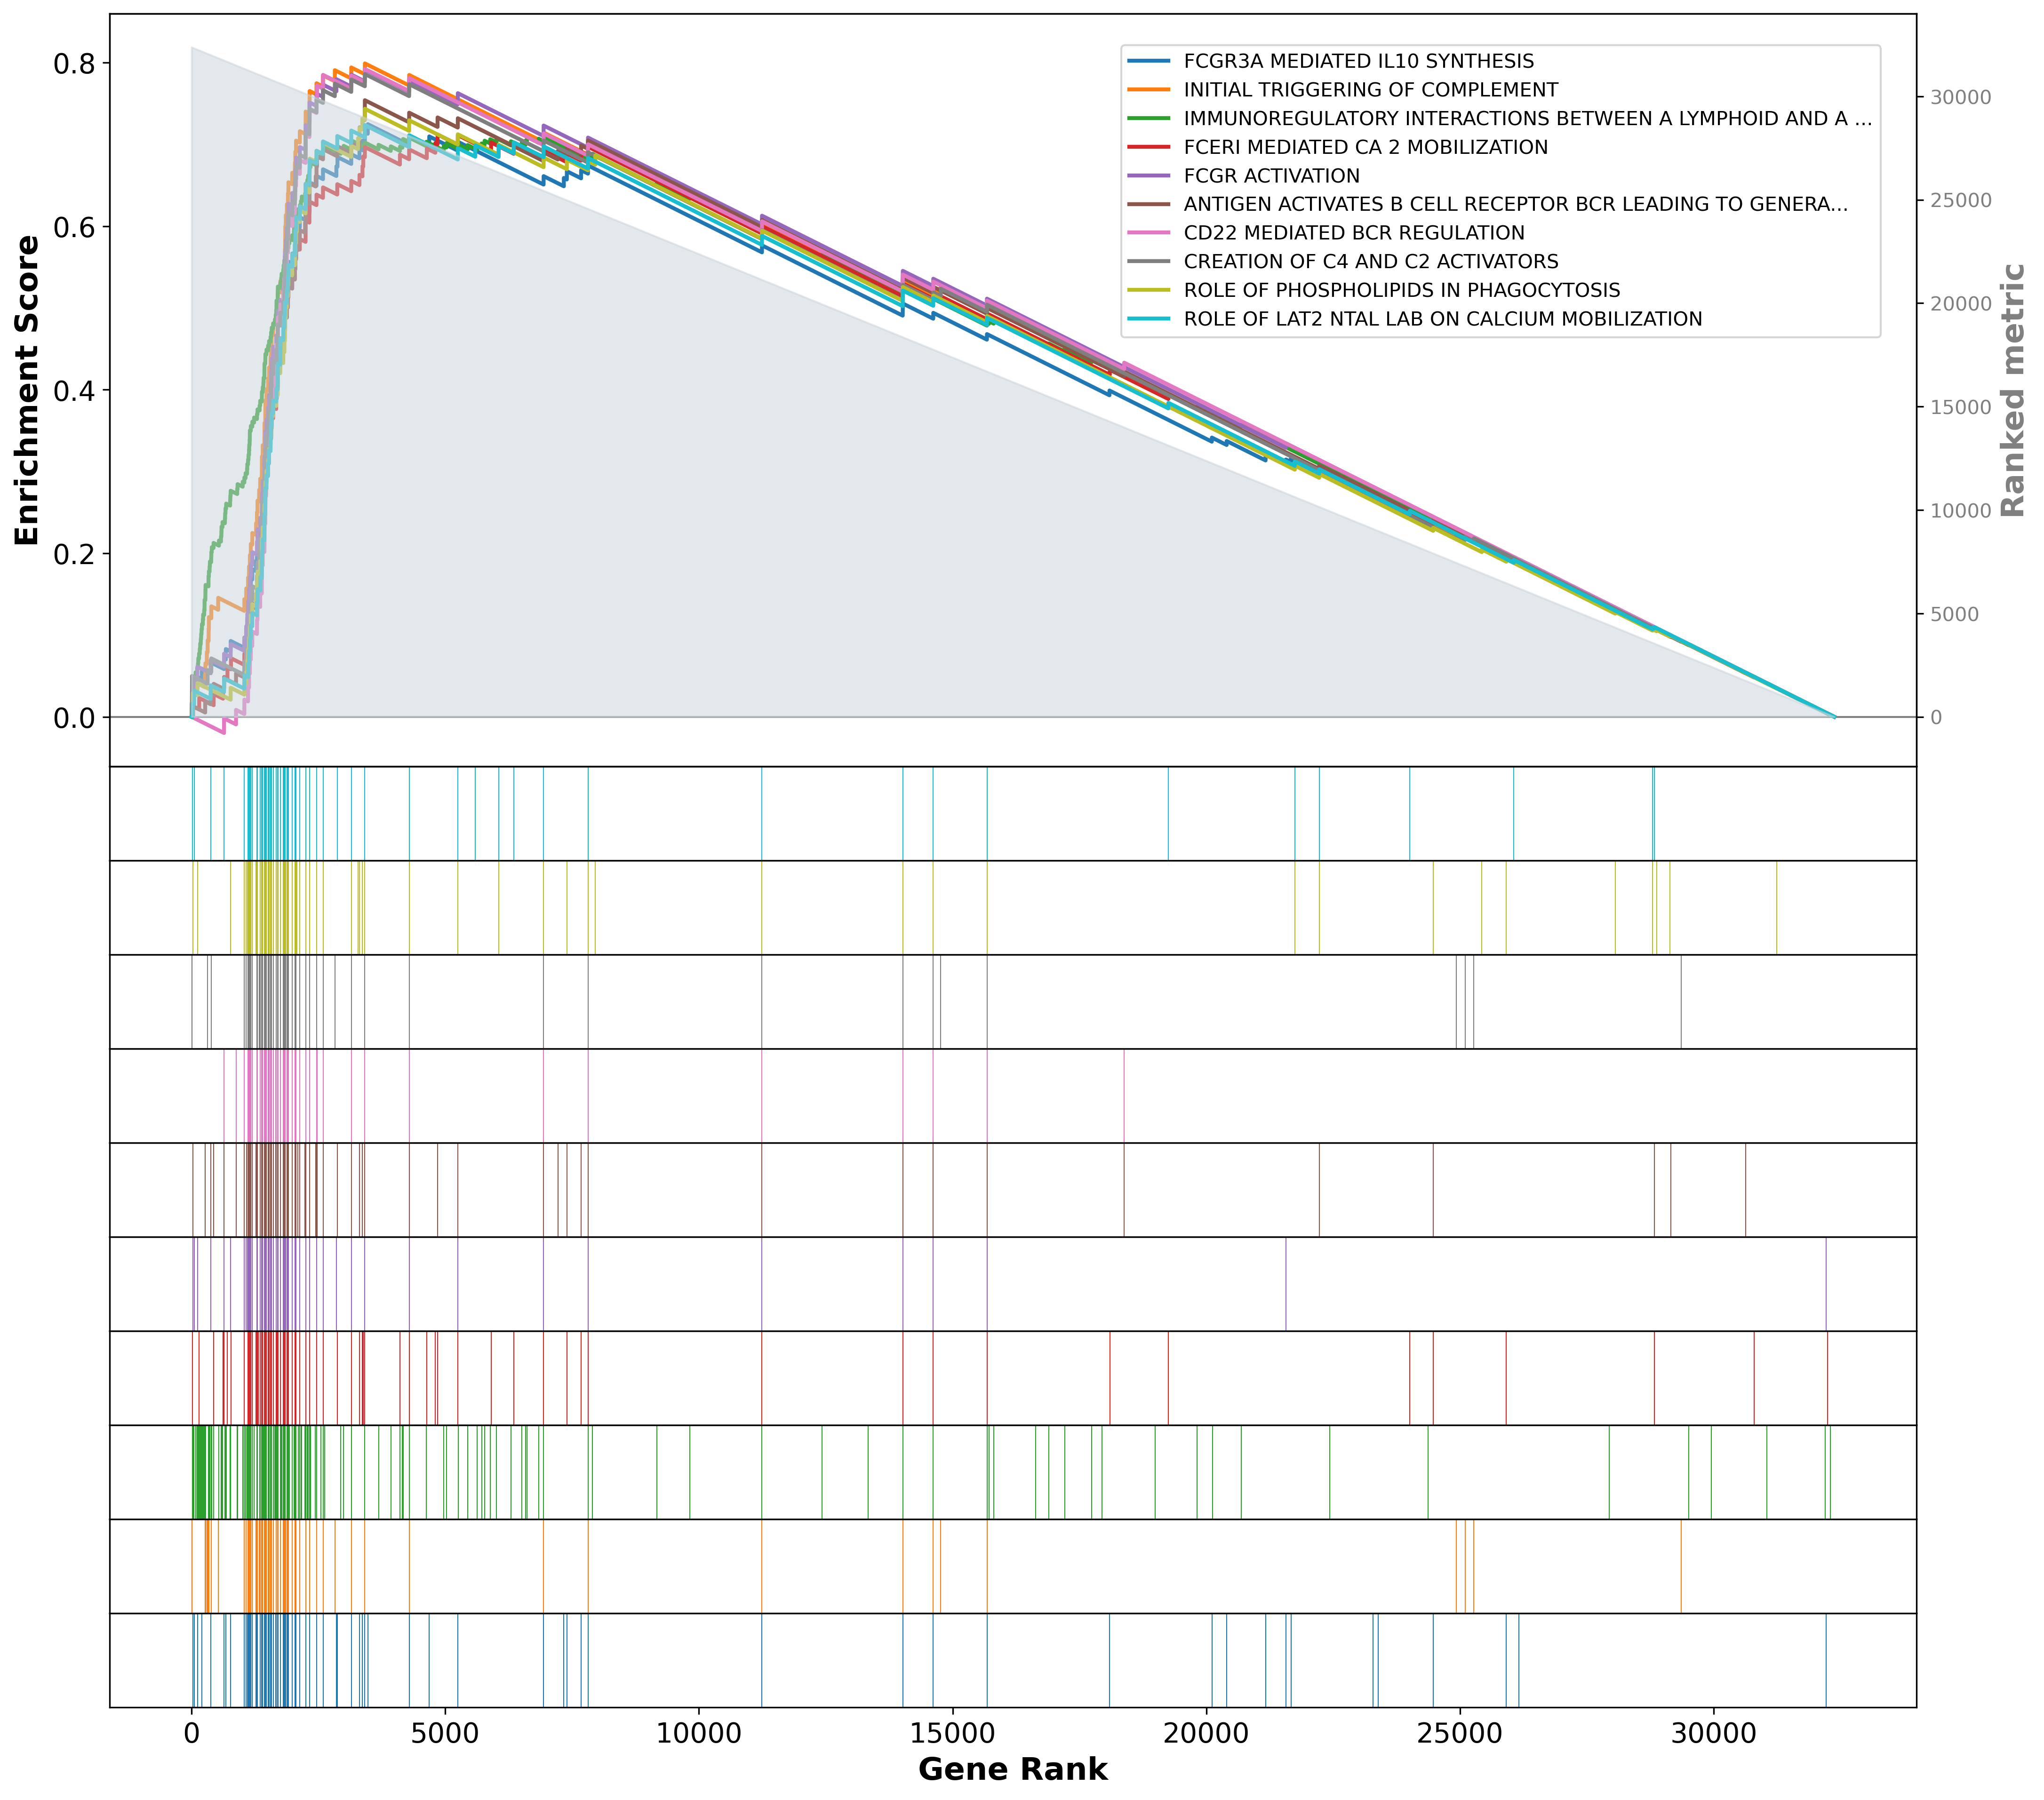
\includegraphics[width=\textwidth,keepaspectratio]{Sections/Network_I/Resources/selective_pruning/gsea/mesLike_10_top_manTerms.png}
%         \caption{Mes-like}
%         \label{fig:ap:gsea_mesLike}
%     \end{subfigure} 
%     \begin{subfigure}[!t]{0.4\textwidth}
%         \centering
%         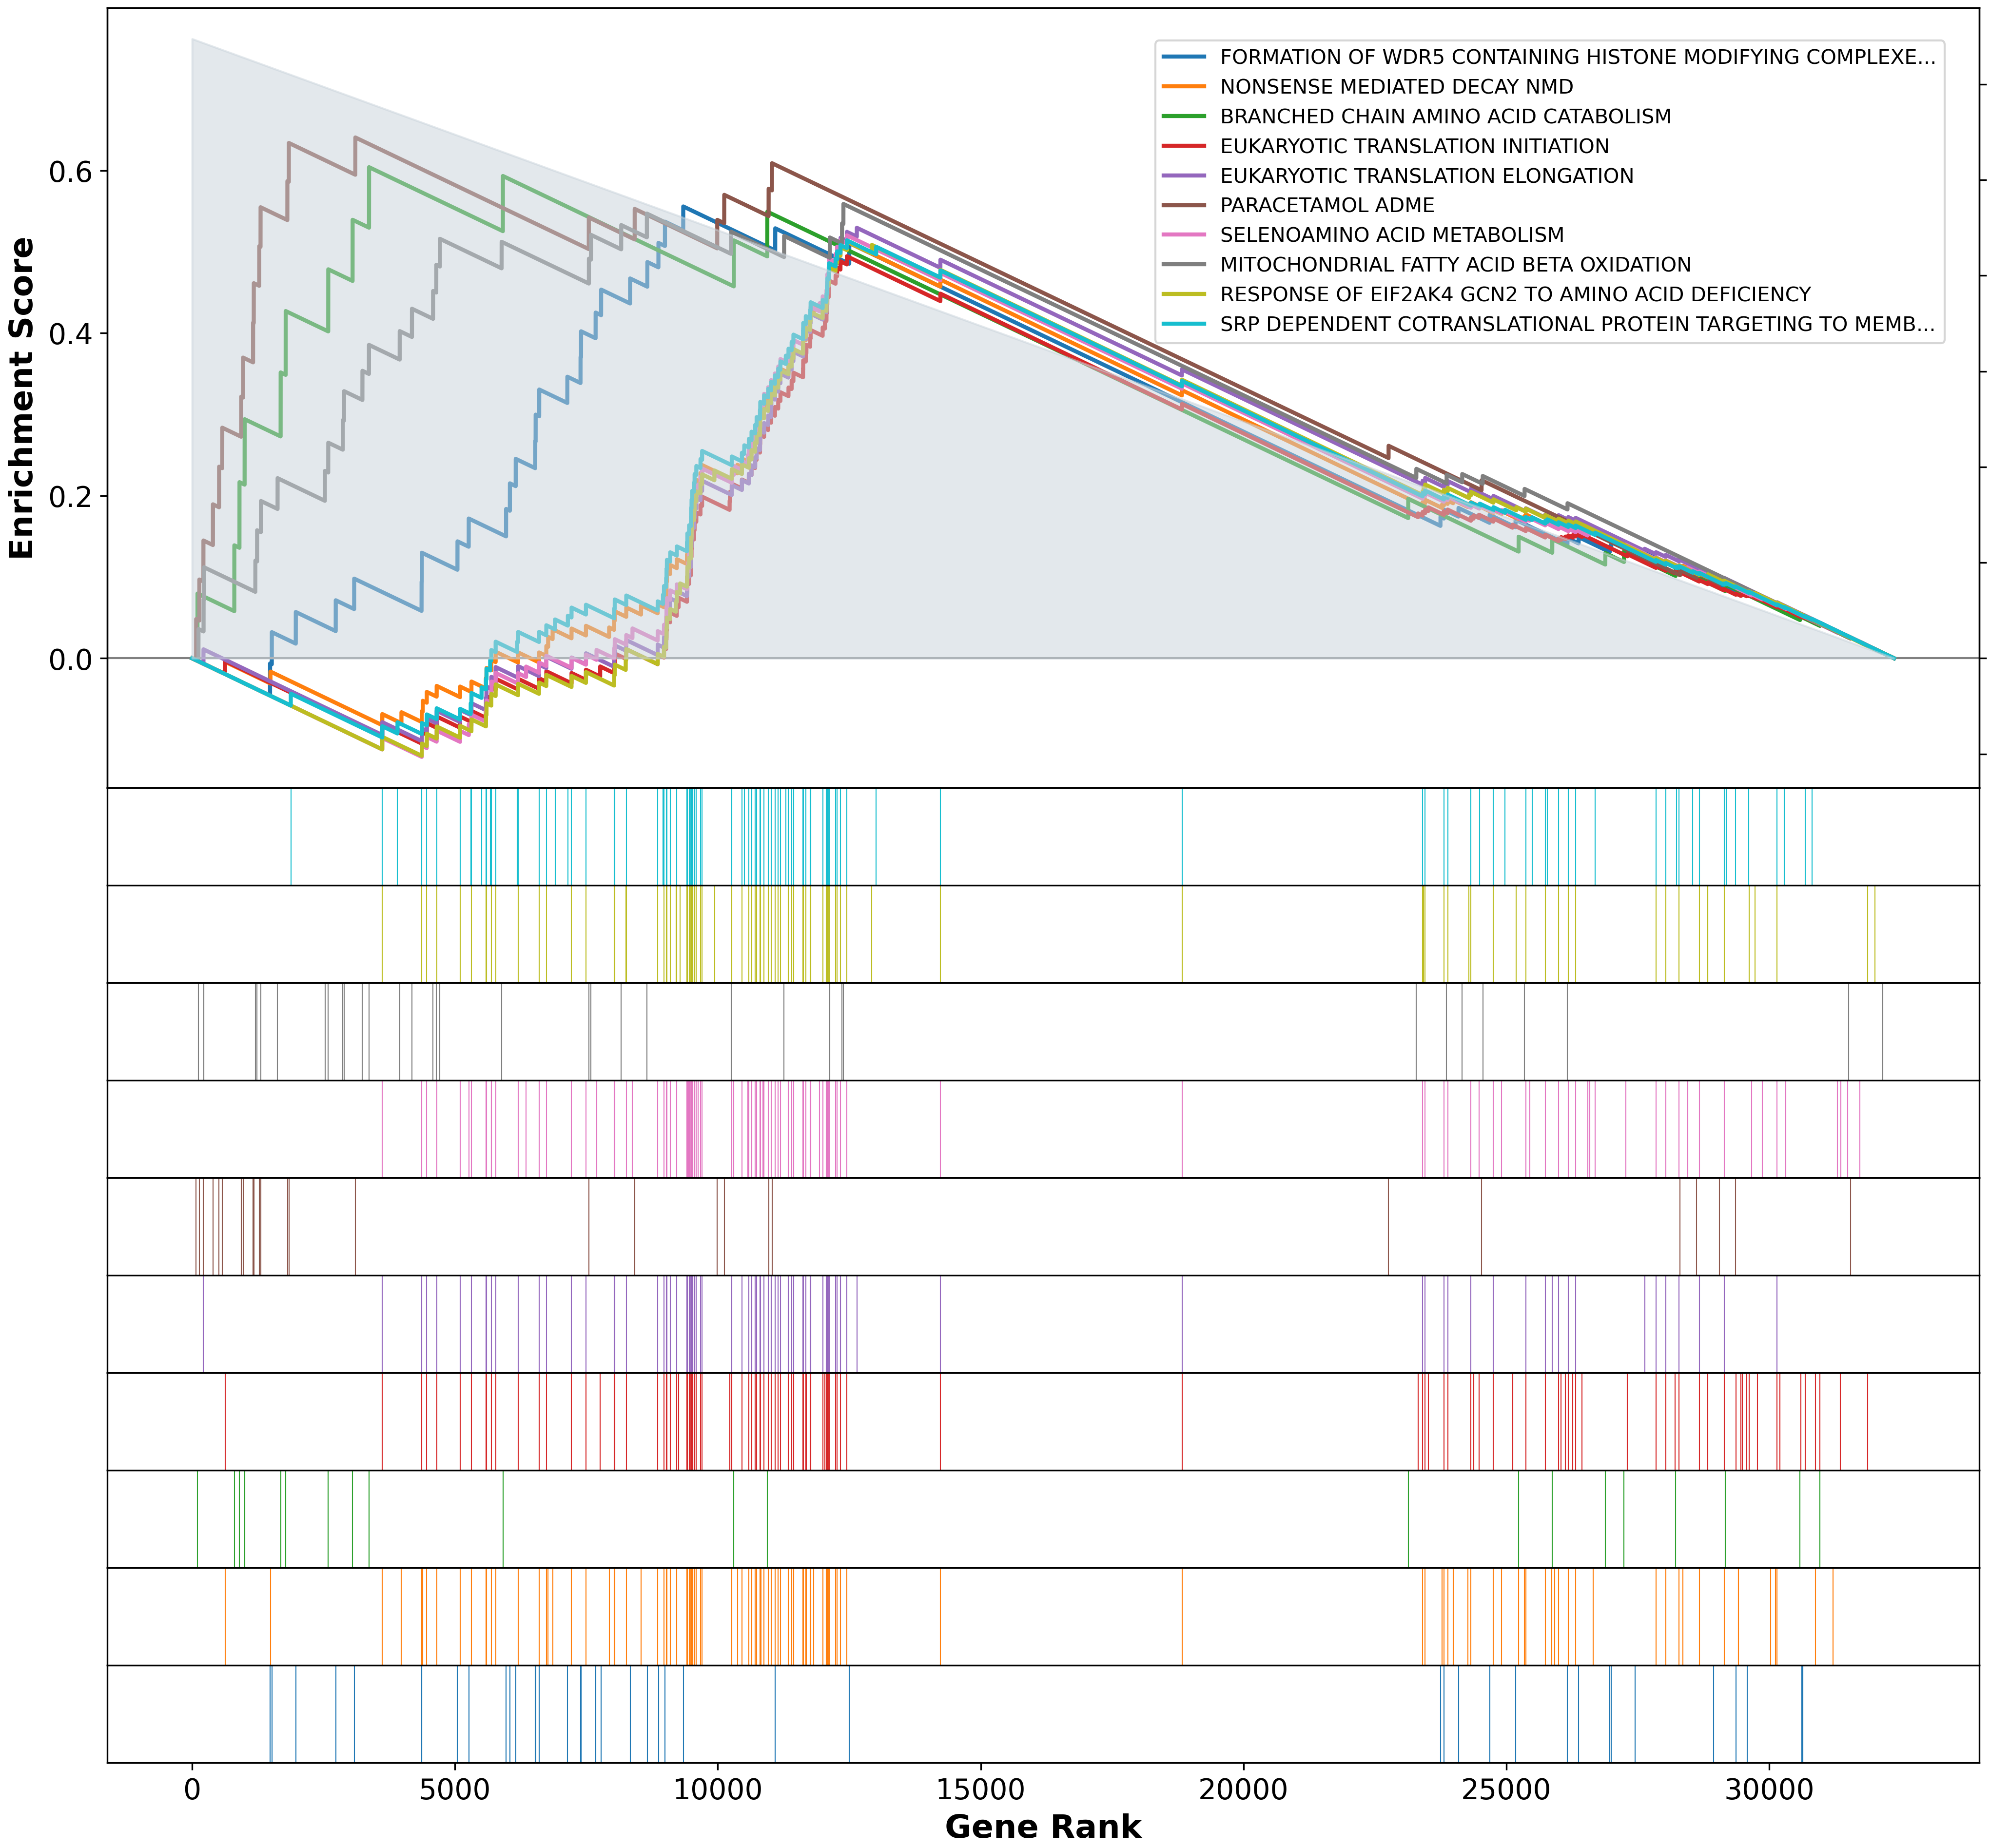
\includegraphics[width=\textwidth,keepaspectratio]{Sections/Network_I/Resources/selective_pruning/gsea/largeLuminal_10_top_manTerms.png}
%         \caption{Large Luminal}
%         \label{fig:ap:gsea_largeLuminal}
%     \end{subfigure}
%     \caption{GSEA output for the groups derived using Selective Edge pruning in  \cref{s:N_I:sel_tfs_subtypes}}
%     \label{fig:ap:gsea_basal}
% \end{figure}



